\documentclass[11pt,a4paper]{report}

% Packages
\usepackage[utf8]{inputenc}
\usepackage[T1]{fontenc}
\usepackage{graphicx}
\usepackage{amsmath, amssymb, amsthm}
\usepackage[style=ieee,backend=biber]{biblatex}
\usepackage{hyperref}
\usepackage{bookmark}
\usepackage{listings}
\usepackage{xcolor}
\usepackage{float}
\usepackage{subcaption}
\usepackage{booktabs}
\usepackage{algorithm}
\usepackage{algorithmic}

% Professional formatting packages
\usepackage[margin=2.5cm]{geometry}  % 1 inch margins (2.5cm)
\usepackage{setspace}                 % Line spacing control
\usepackage{microtype}                % Better typography and spacing
\usepackage{titlesec}                 % Customizable section headings
\usepackage{titletoc}                 % Table of contents formatting
\usepackage{ragged2e}                 % Better text alignment control
\usepackage{needspace}                 % Prevent page breaks before sections
\usepackage{afterpage}                 % Better page break control
\usepackage{enumitem}                 % Better list formatting

% Professional font: Times New Roman (standard for academic theses)
% Use times package and ensure it's the default font family
\usepackage{times}
\renewcommand{\rmdefault}{ptm}  % Times Roman as default roman font
\renewcommand{\sfdefault}{phv}   % Helvetica as default sans-serif
\renewcommand{\ttdefault}{pcr}   % Courier as default typewriter

% ============================================================================
% LINE SPACING: Consistent 1.5x spacing throughout
% ============================================================================
\onehalfspacing

% ============================================================================
% PARAGRAPH FORMATTING: Standard academic indentation
% ============================================================================
\setlength{\parindent}{0.4in}  % Standard paragraph indent
\setlength{\parskip}{0pt}      % No space between paragraphs

% ============================================================================
% TEXT ALIGNMENT: Left-aligned for readability
% ============================================================================
% Ensure Times font is used consistently for body text
\rmfamily
\RaggedRight

% ============================================================================
% ORPHAN/WIDOW CONTROL
% ============================================================================
\widowpenalty=10000
\clubpenalty=10000
\displaywidowpenalty=10000
\brokenpenalty=10000
\interlinepenalty=100
\predisplaypenalty=10000
\postdisplaypenalty=0
\sloppy
\setlength{\emergencystretch}{2em}

% ============================================================================
% PAGE STYLING
% ============================================================================
\pagestyle{plain}

% ============================================================================
% HYPERREF CONFIGURATION
% ============================================================================
\hypersetup{
    colorlinks=true,
    linkcolor=black,
    citecolor=black,
    urlcolor=blue,
    pdfborder={0 0 0}
}

% ============================================================================
% SECTION HEADING FORMATTING: Consistent font sizes
% ============================================================================
% Chapter: 16pt bold, minimal spacing to avoid page breaks (ensure Times font)
\titleformat{\chapter}
  {\rmfamily\fontsize{16}{20}\bfseries\selectfont}
  {\thechapter}{1em}{}
\titlespacing*{\chapter}{0pt}{15pt}{10pt}

% Section: 14pt bold, minimal spacing to avoid page breaks (ensure Times font)
\titleformat{\section}
  {\rmfamily\fontsize{14}{18}\bfseries\selectfont}
  {\thesection}{1em}{}
\titlespacing*{\section}{0pt}{0.8ex plus 0.2ex minus .1ex}{0.6ex plus .1ex}

% Subsection: 12pt bold, consistent spacing (ensure Times font)
\titleformat{\subsection}
  {\rmfamily\fontsize{12}{16}\bfseries\selectfont}
  {\thesubsection}{1em}{}
\titlespacing*{\subsection}{0pt}{0.8ex plus 0.3ex minus .1ex}{0.8ex plus .1ex}

% Prevent page breaks immediately after section headings
% Also ensure font resets to Times after section headings (outside math mode)
% Section redefinitions removed to fix incompatibility with titlesec
% The needspace functionality should be handled via \titlespacing or a safer hook if required.

% ============================================================================
% TABLE OF CONTENTS FORMATTING
% ============================================================================
\titlecontents{chapter}
  [0pt]
  {\addvspace{1pc}\bfseries}
  {\contentslabel{1.5em}}
  {\hspace*{-1.5em}}
  {\titlerule*[.5pc]{.}\contentspage}

% ============================================================================
% TABLE AND FIGURE FORMATTING
% ============================================================================
\renewcommand{\arraystretch}{1.15}  % Slightly reduced for better density
\setlength{\abovecaptionskip}{8pt}
\setlength{\belowcaptionskip}{8pt}

% Ensure figures and tables are properly centered
\makeatletter
\g@addto@macro\@floatboxreset\centering
\renewcommand{\topfraction}{0.85}
\renewcommand{\bottomfraction}{0.85}
\renewcommand{\textfraction}{0.15}
\renewcommand{\floatpagefraction}{0.7}
\makeatother

% ============================================================================
% LIST FORMATTING: Consistent spacing
% ============================================================================
\setlist{
    leftmargin=*,
    itemsep=0.2em,
    parsep=0pt,
    topsep=0.3em,
    before=\needspace{2\baselineskip}
}

% ============================================================================
% CODE LISTING CONFIGURATION: Professional styling (improved)
% ============================================================================
\lstset{
    basicstyle=\ttfamily\fontsize{11}{13.2}\selectfont,  % Minimum 11pt font
    keywordstyle=\color{blue!70!black}\bfseries,
    commentstyle=\color{green!50!black}\itshape,
    stringstyle=\color{red!70!black},
    numbers=left,
    numberstyle=\fontsize{11}{13.2}\selectfont\color{gray!70},
    stepnumber=1,
    numbersep=4pt,
    backgroundcolor=\color{gray!8},
    frame=leftline,  % Left border only for cleaner look
    framerule=1pt,
    rulecolor=\color{gray!40},
    breaklines=true,
    breakatwhitespace=true,
    breakindent=0pt,
    tabsize=2,
    showstringspaces=false,
    captionpos=b,
    aboveskip=6pt,
    belowskip=6pt,
    xleftmargin=12pt,  % Left margin for line numbers
    xrightmargin=4pt
}

\lstdefinelanguage{yaml}{
  keywords={true,false,null,y,n},
  keywordstyle=\color{darkgray}\bfseries,
  basicstyle=\ttfamily\fontsize{9}{11}\selectfont,
  sensitive=false,
  comment=[l]{\#},
  morecomment=[s]{/*}{*/},
  commentstyle=\color{green!50!black}\itshape,
  stringstyle=\color{red!70!black},
  moredelim=[l][\color{orange}]{\&},
  moredelim=[l][\color{magenta}]{*},
  moredelim=**[il][\color{blue!70!black}]{:},
  morestring=[b]',
  morestring=[b]"
}

% Ensure font resets properly after code blocks and inline code
\makeatletter
% Fix lstlisting to reset font after use (prevents font breakage)
\let\oldlstlisting\lstlisting
\let\oldendlstlisting\endlstlisting
\renewenvironment{lstlisting}[1][]
  {\oldlstlisting[#1]}
  {\oldendlstlisting\rmfamily\selectfont\normalsize}

% Ensure verbatim resets font (if any remain)
\let\oldverbatim\verbatim
\let\oldendverbatim\endverbatim
\renewenvironment{verbatim}
  {\oldverbatim}
  {\oldendverbatim\rmfamily\selectfont\normalsize}

% Ensure \texttt properly resets to Times after use (grouped to prevent font leakage)
\let\oldtexttt\texttt
\renewcommand{\texttt}[1]{{\ttfamily\selectfont #1}\rmfamily\selectfont}

% Force Times font at document start and after each section
\AtBeginDocument{\rmfamily\selectfont}
\makeatother

% ============================================================================
% ABSTRACT FORMATTING: Title same size as content
% ============================================================================
% Make "ABSTRACT" title the same size as content (11pt instead of default larger size)
\renewcommand{\abstractname}{\normalsize\bfseries ABSTRACT}

\let\oldabstract\abstract
\let\endoldabstract\endabstract
\renewenvironment{abstract}
  {\oldabstract\onehalfspacing\setlength{\parindent}{0pt}\setlength{\parskip}{0.6em}\rmfamily\fontsize{11}{13.2}\selectfont}
  {\endoldabstract}

% ============================================================================
% REMOVE PARAGRAPH INDENTATION AFTER HEADINGS
% ============================================================================
\makeatletter
\@afterheading
\makeatother

% ============================================================================
% BIBLIOGRAPHY
% ============================================================================
\addbibresource{bib/references.bib}

% ============================================================================
% TITLE PAGE INFORMATION
% ============================================================================
\title{Fraud Detection in Online Real Estate Marketplaces\\Utilizing a Hybrid Graph and Gradient Boosting Model}
\author{Nguyen Hoang Minh}
\date{December 22, 2024}

% Additional title page information
\newcommand{\studentid}{24MSE23152}
\newcommand{\degreeprogram}{Master of Software Engineering}
\newcommand{\supervisor}{Professor Doan Xuan Huy Minh, Ph.D.}
\newcommand{\institution}{FPT School of Business and Technology}
\newcommand{\academicyear}{2024-2025}

\begin{document}

% ============================================================================
% TITLE PAGE: Compact, fits on one page
% ============================================================================
\begin{titlepage}
\centering
\vspace*{1.5cm}

% Title
{\fontsize{18}{22}\bfseries Fraud Detection in Online Real Estate Marketplaces}\\[0.4cm]
{\fontsize{18}{22}\bfseries Utilizing a Hybrid Graph and Gradient Boosting Model}\\[1.5cm]

% Degree statement
{\fontsize{12}{14} A Thesis Submitted in Partial Fulfillment of the\\Requirements for the Degree of}\\[0.4cm]
{\fontsize{14}{18}\bfseries \degreeprogram}\\[1.2cm]

% Author
{\fontsize{12}{14} Submitted by}\\[0.3cm]
{\fontsize{14}{18}\bfseries Nguyen Hoang Minh}\\[0.2cm]
{\fontsize{11}{13.2} Student ID: \studentid}\\[1.2cm]

% Supervisor
{\fontsize{12}{14} Supervised by}\\[0.3cm]
{\fontsize{13}{17} \supervisor}\\[1.2cm]

% Institution
{\fontsize{12}{14} \institution}\\[0.2cm]
{\fontsize{12}{14} Academic Year \academicyear}\\[1cm]

\vfill

\end{titlepage}

\newpage

% ============================================================================
% ABSTRACT
% ============================================================================
\begin{abstract}
Online marketplace fraud causes significant financial losses and erodes user trust. This thesis investigates graph-based fraud pattern discovery in real estate marketplaces, analyzing 804,717 listing events from Swiss Marketplace Group to identify relational fraud signatures and validate their predictive value.

We construct a heterogeneous graph with 31 million edges encoding entity-sharing relationships (device fingerprints, IP addresses, emails, phones) and apply Graph Neural Network-based pattern extraction combined with XGBoost classification. Exploratory analysis reveals distinctive fraud ring structures: super-connector devices (35.5\% fraud rate versus 8.11\% baseline), geographic clustering (West African origins showing 60-90\% fraud rates), and temporal signatures (6-7 AM activity peaks, February 2025 spike).

Model comparison across three independent runs shows GNN+XGBoost achieves mean AUC-PR of 0.733 $\pm$ 0.058, comparable to tabular-only XGBoost (0.733 $\pm$ 0.063), with marginal improvement of 0.08\%. Cross-validation reveals substantial performance degradation (mean 0.28 AUC-PR, 62\% drop) due to temporal distribution shift and decreasing fraud rates (1.97\% to 0.63\%), validating the need for frequent retraining in production deployment. While GNN embeddings contribute 17.3\% of feature importance (SHAP analysis), the primary predictive signal derives from tabular features (82.7\%). Critically, expanding window validation reveals catastrophic GNN degradation (0.22 AUC-PR, 70\% performance loss) under temporal distribution shift, compared to vanilla XGBoost's temporal robustness (0.63 AUC-PR, 86\% retention). This temporal instability limits GNN practical deployment despite supplementary signal in fixed-split evaluation.

Comparison of GNN architectures (GraphSAGE, HGT, CARE-GNN, PC-GNN) identifies GraphSAGE as optimal, though all variants exhibit temporal brittleness. Expanding window analysis establishes that graph patterns require $\sim$300K training samples for meaningful extraction and demonstrates vanilla XGBoost superiority for production deployment requiring frequent retraining. SHAP-based interpretability identifies screen resolution, payment mode, and listing category as top indicators, enabling fraud analyst prioritization through local explanation decomposition.

This research demonstrates that while graph-based pattern discovery reveals fraud ring structures invisible to tabular analysis, the current GNN approach suffers from temporal instability that precludes production deployment. Vanilla XGBoost provides superior operational trade-offs (temporal robustness, computational efficiency), with GNN techniques better suited for offline fraud ring analysis than real-time classification.

\textbf{Keywords:} fraud detection, graph neural networks, data mining, real estate marketplaces, pattern discovery, explainable AI
\end{abstract}

% Remove page breaks between TOC, LOF, LOT, and Abbreviations
% Temporarily disable \cleardoublepage to allow continuous flow
\let\oldcleardoublepage\cleardoublepage
\renewcommand{\cleardoublepage}{}

\tableofcontents
\listoffigures
\listoftables
\chapter*{Abbreviations}
\addcontentsline{toc}{chapter}{Abbreviations}

\begin{description}[leftmargin=3cm, labelwidth=2.5cm, labelsep=0.5cm, style=nextline]
    \item[ADWIN] Adaptive Windowing
    \item[AUC-PR] Area Under the Precision-Recall Curve
    \item[AUC-ROC] Area Under the Receiver Operating Characteristic Curve
    \item[CARE-GNN] Camouflage-Resistant Graph Neural Network
    \item[DDM] Drift Detection Method
    \item[ETL] Extract, Transform, Load
    \item[GNN] Graph Neural Network
    \item[GPU] Graphics Processing Unit
    \item[GraphSAGE] Graph Sample and Aggregation
    \item[HGT] Heterogeneous Graph Transformer
    \item[HPO] Hyperparameter Optimization
    \item[IP] Internet Protocol
    \item[KYC] Know Your Customer
    \item[LIME] Local Interpretable Model-Agnostic Explanations
    \item[LR] Logistic Regression
    \item[ML] Machine Learning
    \item[MLflow] Machine Learning Flow (experiment tracking platform)
    \item[MLP] Multi-Layer Perceptron
    \item[PC-GNN] Pick and Choose Graph Neural Network
    \item[PII] Personally Identifiable Information
    \item[PIT] Point-in-Time
    \item[PyG] PyTorch Geometric
    \item[PyTorch] Python Tensor Library
    \item[RF] Random Forest
    \item[RQ] Research Question
    \item[SHAP] SHapley Additive exPlanations
    \item[SMG] Swiss Marketplace Group
    \item[SQL] Structured Query Language
    \item[VPN] Virtual Private Network
    \item[XAI] Explainable Artificial Intelligence
    \item[XGBoost] eXtreme Gradient Boosting
    \item[YAML] YAML Ain't Markup Language
\end{description}


% Restore \cleardoublepage for the rest of the document
\let\cleardoublepage\oldcleardoublepage

\chapter{Introduction}
\label{ch:introduction}

\section{Background and Motivation}
\label{sec:1_1}

The proliferation of online marketplaces has fundamentally transformed how consumers search for and secure housing. In Switzerland alone, platforms such as Homegate and ImmoScout24, operated by Swiss Marketplace Group (SMG), facilitate hundreds of thousands of real estate transactions annually. However, this digital transformation has simultaneously created fertile ground for sophisticated fraud schemes, generating complex data environments where fraudulent patterns are embedded within massive transaction graphs.

Real estate fraud in online marketplaces manifests in several forms: phantom listings advertising non-existent properties, identity theft schemes harvesting applicant information, and coordinated fraud rings operating networks of fake accounts. These fraud operations leave distinctive traces in marketplace data shared device fingerprints, IP address clusters, temporal posting patterns, and entity relationship networks that are invisible when analyzing listings in isolation but become apparent through systematic data mining.

Traditional fraud detection approaches treat listings as independent observations, applying rule-based systems or commercial services such as SEON that analyze individual transactions without exploiting relational structure. While these approaches capture obvious fraud indicators (disposable emails, high-risk IP countries), they cannot discover the network patterns that distinguish fraud rings from legitimate property management operations.

Despite the maturity of graph-based fraud detection in adjacent domains---with over 100 publications applying Graph Neural Networks to financial transactions \cite{cheng2024gnn}, production deployments at e-commerce platforms processing billions of transactions (eFraudCom at Taobao, C-FATH at JD.com), and standardized benchmark datasets (YelpChi, Elliptic)---no academic research has applied these methods to real estate marketplace fraud. A systematic review of fraud detection literature reveals this absence: Mutemi and Bação's \cite{mutemi2024ecommerce} survey of 101 e-commerce fraud publications excludes real estate entirely; Cherif et al.'s \cite{cherif2024financial} systematic review of GNN-based financial fraud detection covers credit cards, money laundering, and insurance but omits property marketplaces; the only peer-reviewed real estate fraud study \cite{mohdamin2024clustering} employs traditional clustering rather than graph methods. This gap persists despite documented fraud losses exceeding \$145 million annually in real estate scams \cite{fbi2023ic3} and the inherent relational structure of marketplace data---agent networks, cross-platform listing patterns, device-sharing graphs---that suggests graph methods would be highly applicable.

This thesis addresses this gap by applying graph-based data mining techniques to discover, characterize, and validate fraud patterns in real estate marketplace data. By constructing heterogeneous graphs from entity relationships and applying graph-based pattern extraction, we aim to uncover relational fraud signatures invisible to attribute-only analysis, while investigating the unique structural properties of fraud in this unexplored domain.

\section{Research Objectives and Questions}
\label{sec:1_2}

The primary objective of this thesis is to discover, characterize, and validate relational fraud patterns in real estate marketplace data through graph-based data mining, demonstrating their utility for improved fraud detection and operational investigation support.

This objective is operationalized through four research questions:

\textbf{RQ1: What relational fraud patterns exist in marketplace graphs, and do they provide predictive signal beyond individual listing attributes?}

This question addresses pattern discovery and validation. By constructing heterogeneous graphs from entity relationships and extracting relational representations, we identify structural patterns distinguishing fraudulent from legitimate listings. Comparison between graph-augmented and attribute-only models validates whether discovered patterns carry predictive information.

\textbf{RQ2: What entity-sharing patterns characterize fraud rings versus legitimate multi-listing users?}

Beyond aggregate pattern detection, this question examines the specific topological and behavioral signatures of coordinated fraud operations. We analyze device-sharing networks, IP clustering, email/phone reuse patterns, and temporal coordination to characterize fraud ring structure versus legitimate property management behavior.

\textbf{RQ3: How do fraud patterns evolve temporally, and what data requirements enable effective pattern discovery?}

Fraud patterns are non-stationary; fraudsters adapt tactics over time. This question examines temporal evolution of fraud signatures and, critically, identifies the minimum data scale at which graph-based patterns emerge as predictive. Through expanding window analysis, we quantify data requirements for effective pattern mining.

\textbf{RQ4: What actionable fraud indicators emerge from pattern analysis that can support human investigation?}

Discovered patterns must translate to operational value. This question examines which features both individual attributes and relational patterns most strongly indicate fraud, producing interpretable indicators that fraud analysts can use to prioritize and guide investigations.

\section{Scope and Delimitations}
\label{sec:1_3}

This research is conducted as a case study utilizing production data from Swiss Marketplace Group's real estate platforms.

\textbf{In Scope:}
\begin{itemize}
    \item Exploratory analysis of marketplace data structure and fraud distributions
    \item Construction of heterogeneous entity-relationship graphs from listing data
    \item Graph-based pattern extraction using Graph Neural Network techniques
    \item Validation of pattern utility through predictive modeling comparison
    \item Temporal pattern analysis through expanding window experiments
    \item Interpretability analysis to identify actionable fraud indicators
\end{itemize}

\textbf{Out of Scope:}
\begin{itemize}
    \item Real-time streaming analysis (batch processing focus)
    \item Unstructured content mining (listing text, images)
    \item Cross-marketplace pattern transfer
    \item Fully dynamic graph representations
\end{itemize}

\textbf{Delimitations:}
\begin{itemize}
    \item Patterns reflect Swiss real estate market characteristics; generalization requires validation
    \item Ground truth derives from operational flagging, which may contain labeling noise
    \item Proprietary data constraints limit reproducibility; statistical summaries provided
\end{itemize}

\section{Research Contributions}
\label{sec:1_4}

This thesis makes contributions to both the data mining research literature and operational fraud detection practice at Swiss Marketplace Group.

\subsection*{Academic Contributions}

\textbf{Contribution 1: Discovery of the Heterophily Paradox in Real Estate Fraud Graphs.}
We discover that real estate marketplace graphs exhibit \emph{inverted} fraud topology compared to assumptions in the graph fraud detection literature. While existing work assumes fraudsters form densely connected clusters requiring camouflage-resistant methods \cite{dou2020enhancing,liu2020alleviating}, our analysis reveals the opposite pattern: legitimate property managers form dense entity-sharing networks (5.3\% fraud rate for devices with 5+ listing connections), while fraudsters operate in relative isolation (16.7\% fraud rate for single-listing devices). This heterophily pattern---where high connectivity signals legitimacy rather than fraud---explains why standard GNN architectures underperform in this domain and represents the first empirical characterization of fraud network structure in real estate marketplaces.

\textbf{Contribution 2: Establishment of Graph Density Threshold for Relational Pattern Mining.}
Through systematic expanding window analysis, we provide the first empirical quantification of data requirements for graph-based fraud pattern discovery. Graph mining provides predictive lift over attribute-only analysis only when training data exceeds approximately 300,000 samples---the threshold at which fraud ring connectivity reaches sufficient density to overcome legitimate power-user noise. Below this threshold, relational patterns lack structural coherence for meaningful extraction. This finding addresses a methodological gap in the literature: prior work demonstrates graph patterns improve detection but does not investigate \emph{when} this occurs, leaving practitioners unable to assess graph-based approach viability for their data contexts.

\textbf{Contribution 3: Demonstration of Temporal Robustness Inversion Under Production Evaluation.}
We demonstrate that evaluation methodology fundamentally determines model selection conclusions in fraud detection. Under fixed-split evaluation (standard academic benchmark), graph-augmented models achieve +5.3\% AUC-PR improvement over tabular baselines. However, under expanding window evaluation (production deployment scenario with periodic retraining), this relationship inverts: tabular models outperform graph-augmented approaches by 3$\times$ (0.63 vs. 0.22 AUC-PR). This discovery reveals that fraud evolution operates at the \emph{topology level}---new fraud campaigns form disconnected graph components with distinct structures---not merely at the feature distribution level assumed in prior concept drift literature \cite{gama2014survey}. We identify two operational regimes: forensic analysis (offline, large historical graphs) where GNN methods excel, and real-time detection (incremental retraining) where tabular methods provide superior robustness.

\subsection*{Practical Contributions}

\textbf{Contribution 4: Complementary Detection Layer for Existing Fraud Systems.}
The discovered patterns enable a secondary detection mechanism operating alongside SMG's existing SEON-based fraud detection. Unlike SEON's rule-based approach analyzing individual transactions, the graph-based system identifies fraud through relational signatures---detecting coordinated activity invisible to single-listing analysis. This provides both forward detection (risk scoring at submission) and backward detection (retrospective identification of published fraud based on emerging entity-sharing patterns from subsequent user activity).

\textbf{Contribution 5: Empirically-Validated Rule Enhancement.}
The characterized patterns---super-connector thresholds (10+ listings per device yields 35.5\% fraud rate, 4.4$\times$ baseline), cross-platform signatures (dual Homegate/ImmoScout24 posting yields 26.74\% fraud rate), temporal indicators (6-7 AM submission peaks), and geographic concentration (West African origin patterns showing 60-90\% fraud rates)---provide empirically quantified signals for SEON rule enhancement. Each pattern includes precision metrics enabling risk-calibrated rule implementation rather than heuristic thresholds.

\section{Thesis Organization}
\label{sec:1_5}

The remainder of this thesis is organized as follows:

\textbf{Chapter 2: Literature Review} surveys related work in graph-based pattern mining, anomaly detection in networks, fraud detection methodologies, and interpretable machine learning, positioning this research within the data mining literature.

\textbf{Chapter 3: Methodology} details the data mining approach including exploratory data analysis, graph construction methodology, pattern extraction techniques, validation experimental design, and temporal analysis protocols.

\textbf{Chapter 4: Implementation} describes technical realization including data pipelines, graph construction, pattern extraction via Graph Neural Networks, and pattern validation.

\textbf{Chapter 5: Results and Analysis} presents discovered patterns organized by research question: relational structures (RQ1), fraud ring characteristics (RQ2), temporal evolution and data requirements (RQ3), and actionable indicators (RQ4). The chapter concludes with interpretation of findings and practical recommendations.

\textbf{Chapter 6: Conclusion and Future Work} summarizes contributions, examines limitations, and identifies directions for extended pattern discovery research.

\chapter{Literature Review}
This chapter surveys the theoretical foundations and related work underpinning the pattern discovery approach developed in this thesis. The review is organized around a data mining perspective: techniques for discovering patterns in graph-structured data, followed by methods for validating their utility. Coverage spans graph mining fundamentals, fraud-specific patterns, hybrid validation approaches, and methodological considerations including class imbalance, temporal validation, and interpretability.

Throughout, emphasis is placed on pattern discovery as the primary goal, with machine learning serving as a validation mechanism rather than an end in itself.

\section{Graph-Based Pattern Mining and Anomaly Detection}
\label{sec:2_2}

Relational data---where entities connect through diverse relationships---requires analytical approaches that explicitly model network structure. This section reviews graph mining fundamentals, network anomaly detection, and Graph Neural Networks as tools for extracting relational patterns.

\subsection{Graph Mining Fundamentals}

Graph mining encompasses techniques for discovering structural patterns within network data. Three foundational approaches inform fraud pattern discovery.

\textbf{Community detection} identifies densely connected subgroups within larger networks. Methods range from modularity optimization \cite{newman2006modularity} to spectral clustering and label propagation. In fraud contexts, communities may represent fraud rings---groups of accounts or listings with unusually dense interconnections through shared devices, IPs, or behavioral patterns. \citeauthor{akoglu2015graph} \cite{akoglu2015graph} surveyed graph-based anomaly detection, noting that fraud rings often form near-cliques that stand out against the sparse connectivity of legitimate user behavior.

\textbf{Link analysis and centrality measures} quantify node importance within network structure. PageRank, betweenness centrality, and degree distributions reveal nodes occupying unusual structural positions. In marketplace fraud, super-connector entities---devices linked to thousands of listings---represent clear centrality anomalies. \citeauthor{savage2014anomaly} \cite{savage2014anomaly} demonstrated that centrality-based features significantly improve fraud detection in online auction networks.

\textbf{Subgraph pattern mining} discovers recurring structural motifs that may indicate specific behaviors. Frequent subgraph mining techniques \cite{jiang2013survey} identify common local patterns, while graph kernels measure similarity between subgraphs. Fraud operations often exhibit characteristic motifs: star patterns (one device connecting many listings), chains (sequential account creation), or dense cores with peripheral legitimate connections for camouflage.

\subsection{Anomaly Detection in Networks}

Network anomaly detection identifies entities or structures deviating from expected patterns. Anomalies relevant to fraud manifest at multiple levels.

\textbf{Structural anomalies} involve unusual connectivity patterns. A listing connected to a device that links to hundreds of other listings exhibits structural anomaly regardless of its individual attributes. \citeauthor{akoglu2015graph} \cite{akoglu2015graph} categorized structural anomalies into static patterns (unusual degree, clustering coefficient) and dynamic patterns (sudden connectivity changes). For fraud detection, both matter: established fraud rings show static structural signatures, while emerging operations create dynamic anomalies.

\textbf{Attribute-based anomalies} occur when node features deviate from neighbors or population norms. A listing with legitimate-appearing attributes connected to nodes with high-risk characteristics (disposable emails, VPN usage, suspicious geographic origins) represents an attribute anomaly in graph context---its individual features are normal, but its relational context is suspicious.

\textbf{Collective anomalies} involve groups of entities that are individually unremarkable but collectively suspicious. Fraud rings exemplify collective anomalies: each fake listing may appear plausible in isolation, but their coordinated timing, shared infrastructure, and similar content reveal the collective pattern. \citeauthor{noble2003graph} \cite{noble2003graph} pioneered graph-based collective anomaly detection, demonstrating that relational context dramatically improves detection of coordinated malicious activity.

\citeauthor{ranshous2015anomaly} \cite{ranshous2015anomaly} surveyed anomaly detection in dynamic graphs, emphasizing that temporal context enhances pattern detection---a sudden burst of listings from a new device cluster is more suspicious than gradual growth from established accounts.

\subsection{Graph Neural Networks as Pattern Extractors}

Graph Neural Networks (GNNs) provide a learnable approach to extracting patterns from network structure, complementing traditional graph mining with adaptive representation learning.

\textbf{Representation learning} transforms graph structure into dense vector embeddings that encode relational patterns. Unlike hand-crafted graph features (degree, centrality, clustering coefficient), relational pattern representations are learned end-to-end to optimize downstream tasks. \citeauthor{hamilton2017inductive} \cite{hamilton2017inductive} introduced GraphSAGE, which learns to aggregate neighborhood information through trainable functions:

\begin{equation}
\mathbf{h}_v^{(l)} = \sigma\left(\mathbf{W} \cdot \text{AGG}\left(\{\mathbf{h}_u^{(l-1)} : u \in \mathcal{N}(v)\}\right)\right)
\end{equation}

where the aggregation function AGG learns which neighborhood patterns are relevant. This formulation automatically discovers structural patterns predictive of the target task---in fraud detection, patterns distinguishing fraudulent from legitimate entity-sharing networks.

\textbf{Message passing as pattern aggregation} provides the conceptual framework for understanding GNN operation. Each layer aggregates information from neighboring nodes, progressively capturing patterns at increasing structural distances. A two-layer GNN captures patterns involving second-degree connections: a listing shares a device with another listing that shares an email with a known fraud account. \citeauthor{gilmer2017neural} \cite{gilmer2017neural} unified diverse GNN architectures under the message passing framework, clarifying their role as learnable pattern aggregators.

\textbf{Inductive capability} enables pattern extraction for new entities without retraining. Unlike transductive methods that require the full graph at training time, GraphSAGE and similar architectures learn aggregation functions that generalize to unseen nodes. For fraud detection, this is essential: new listings must be scored immediately using patterns learned from historical data. The model learns "if a new listing shares devices with entities exhibiting these patterns, assign similar representation"---transferring discovered patterns to novel entities.

Importantly, GNNs in this thesis serve as pattern extraction tools rather than end-to-end classifiers. The extracted embeddings encode relational patterns which are then validated through classification models, enabling both pattern discovery and interpretability analysis.

\section{Fraud Pattern Discovery in Transaction Networks}
\label{sec:2_3}

While Section 2.2 established general graph mining foundations, fraud detection presents domain-specific challenges arising from adversarial behavior. This section examines entity-relationship patterns characteristic of fraud operations and the challenges fraudsters' deliberate camouflage poses for pattern extraction.

\subsection{Entity-Relationship Patterns in Fraud}

Fraud operations leave distinctive relational signatures across multiple entity types. Understanding these patterns is prerequisite to effective mining.

\textbf{Device and IP sharing networks} provide the strongest fraud signals in marketplace contexts. Legitimate users typically operate from one or few devices; fraud rings share infrastructure across many fake accounts. \citeauthor{vanvlasselaer2015apate} \cite{vanvlasselaer2015apate} demonstrated that device-sharing graphs reveal coordinated fraud invisible to transaction-level analysis, with fraud rings forming dense clusters in device-account bipartite graphs. IP address patterns are noisier---legitimate users may share corporate or residential IPs---but unusual IP-to-account ratios and geographic inconsistencies (account claims Swiss residence but connects from West Africa) provide complementary signal.

\textbf{Temporal coordination patterns} distinguish automated fraud operations from organic user behavior. Fraud rings often exhibit synchronized activity: multiple listings created within narrow time windows, similar posting schedules across accounts, or rapid sequential actions suggesting scripted behavior. \citeauthor{cao2012aiding} \cite{cao2012aiding} formalized "lockstep behavior" detection, identifying accounts with suspiciously similar temporal activity patterns as likely coordinated. In real estate marketplaces, coordinated listing creation across multiple fake accounts represents a characteristic temporal pattern.

\textbf{Cross-platform fraud signatures} emerge when fraudsters maximize exposure by posting across multiple platforms. While legitimate property managers may also cross-post, the combination of cross-platform presence with other risk indicators (new accounts, suspicious infrastructure) amplifies fraud signal. Platform-sharing patterns, combined with content similarity analysis, can reveal fraud campaigns operating across marketplace boundaries.

\textbf{Email and phone reuse patterns} reveal account relationships that users attempt to hide. While fraudsters typically create distinct email addresses per account, patterns emerge: similar naming conventions, shared email domains, or sequential registration. Phone number sharing is particularly revealing, as phone numbers are harder to obtain at scale than email addresses. \citeauthor{hooi2016fraudar} \cite{hooi2016fraudar} demonstrated that sparse identity-sharing graphs, when properly analyzed, reveal fraud networks that dense transaction graphs obscure.

\subsection{The Heterophily Challenge}

A fundamental challenge for graph-based fraud detection is that fraudsters deliberately manipulate graph structure to evade detection---a phenomenon creating heterophily in fraud graphs.

Standard graph mining assumes \textbf{homophily}: connected entities share similar properties. Community detection, label propagation, and GNN message passing all leverage this assumption. However, sophisticated fraudsters establish connections with legitimate users to camouflage their activities. A fake listing may share an IP with hundreds of legitimate listings from a corporate network. A fraudulent account may interact with popular legitimate sellers to build apparent credibility.

\citeauthor{dou2020enhancing} \cite{dou2020enhancing} formalized this as the \textbf{camouflage problem}, demonstrating that fraud graphs exhibit strong heterophily---fraudulent nodes have majority-legitimate neighborhoods. When pattern extraction methods aggregate neighbor information, the fraud signal becomes diluted. \citeauthor{liu2020alleviating} \cite{liu2020alleviating} quantified this on benchmark datasets: over 90\% of fraudulent nodes have majority-legitimate neighbors, causing standard aggregation to actively harm pattern extraction.

This heterophily has implications for pattern discovery methodology:

\textbf{Pattern-preserving approaches} modify aggregation to maintain fraud signal despite mixed neighborhoods. CARE-GNN \cite{dou2020enhancing} employs reinforcement learning to select informative neighbors while filtering camouflage connections. PC-GNN \cite{liu2021heterogeneous} uses label-balanced sampling to ensure fraud patterns receive adequate representation during learning. These methods achieve 2--5\% improvement over standard approaches on fraud benchmarks by preserving rather than smoothing distinctive fraud patterns.

\textbf{Spectral perspectives} reveal that fraud manifests as high-frequency graph signals---rapid label changes between connected nodes---that standard low-pass GNN filters suppress. \citeauthor{tang2022rethinking} \cite{tang2022rethinking} demonstrated that frequency-adaptive methods capturing high-frequency components significantly improve fraud pattern extraction.

The practical implication is that naive application of graph methods may perform worse than ignoring graph structure entirely. Effective fraud pattern mining requires methods designed for adversarial, heterophilic graph contexts.

\subsection{Industrial Pattern Discovery}

Academic benchmarks, while valuable, may not capture patterns at production scale. Industrial deployments provide crucial validation that graph-based pattern discovery delivers operational value.

\textbf{Alibaba's GEM system} \cite{liu2018heterogeneous} demonstrated graph-based pattern discovery at massive scale, analyzing account-device-merchant graphs for the world's largest mobile payment platform. The system identified fraud rings invisible to transaction-level analysis, with graph patterns providing the primary detection signal for coordinated fraud.

\textbf{eBay's BRIGHT system} \cite{ebay2022bright} emphasized that practical pattern discovery requires infrastructure supporting real-time scoring. Their Lambda architecture combines batch-computed graph patterns with streaming updates, enabling pattern-based scoring within latency constraints.

\textbf{Grab's fraud detection platform} \cite{khoo2024building} documented a critical insight: graph construction quality often matters more than analytical sophistication. Their ablation studies revealed that 60--70\% of performance gains came from improved graph design---adding edge types, refining temporal windows, adjusting identity resolution---rather than pattern extraction methodology. This finding emphasizes that data preparation is foundational to pattern discovery.

These industrial experiences inform the methodology developed in this thesis: emphasis on careful graph construction, pattern-preserving extraction methods, and validation that discovered patterns genuinely improve detection.

\subsection{Recent Comprehensive Reviews}

Recent systematic reviews have consolidated the growing body of research on graph-based fraud detection. \citeauthor{motie2024financial} \cite{motie2024financial} provide a comprehensive survey of GNN applications in financial fraud detection, proposing a unified framework that categorizes existing methodologies. Their analysis reveals that GNNs are exceptionally adept at capturing complex relational patterns and dynamics within financial networks, significantly outperforming traditional fraud detection methods. The review identifies key research directions including temporal GNNs for evolving fraud patterns, federated learning approaches for privacy-preserving fraud detection, and adaptive methods for handling concept drift.

This consolidation of evidence provides strong motivation for the graph-based pattern discovery approach developed in this thesis, while highlighting the importance of addressing heterophily, temporal dynamics, and interpretability---all considerations incorporated into our methodology.

\section{Hybrid Approaches: Pattern Extraction and Validation}
\label{sec:2_4}

Discovered relational patterns require validation to confirm their predictive utility. This section examines two-stage approaches that separate pattern extraction from classification, enabling both effective detection and interpretable analysis of what patterns drive predictions.

\subsection{Two-Stage Pattern Mining}

The hybrid approach decomposes fraud detection into distinct phases: pattern extraction and pattern validation.

\textbf{Pattern extraction} transforms graph structure into dense representations encoding relational patterns. Graph Neural Networks, as described in Section 2.2.3, learn embeddings where structurally similar nodes (those sharing connectivity patterns, neighborhood characteristics, or multi-hop relationships) receive similar representations. These embeddings encode patterns such as ``connected to high-degree device nodes,'' ``part of a temporal cluster of new listings,'' or ``shares identity markers with flagged accounts'' without requiring manual pattern specification.

\textbf{Pattern validation} combines extracted patterns with individual entity attributes for classification. Gradient Boosting methods XGBoost \cite{chen2016xgboost} and LightGBM \cite{ke2017lightgbm} excel at this task due to native handling of mixed feature types, robustness to missing values, and built-in interpretability through feature importance. The enriched feature vector concatenates original attributes with extracted pattern representations:

\begin{equation}
\mathbf{f}_v = [\mathbf{x}_v \| \mathbf{z}_v]
\end{equation}

where $\mathbf{x}_v$ represents individual listing attributes (price, category, SEON signals) and $\mathbf{z}_v$ represents GNN-extracted relational patterns. Classification performance on this enriched vector validates whether discovered patterns carry predictive signal beyond individual attributes.

\textbf{Advantages of separation} include independent development and debugging of each stage, cached pattern representations for efficient inference, and direct application of SHAP to the final classifier for interpretability. \citeauthor{grinsztajn2022why} \cite{grinsztajn2022why} demonstrated that tree-based methods outperform deep learning on medium-sized tabular data the regime of most fraud applications supporting the choice of XGBoost for validation rather than end-to-end neural classification.

\subsection{Evidence from Prior Work}

Empirical evidence supports the two-stage approach across fraud detection domains.

\textbf{Intel's reference implementation} \cite{intel2023credit} for credit card fraud demonstrated that GraphSAGE embeddings combined with XGBoost achieved 3-5\% AUC-PR improvement over XGBoost alone. Critically, their self-supervised pretraining using link prediction rather than fraud labels for GNN training extracted patterns capturing general graph structure, which proved predictive of fraud without explicit supervision. This supports the view that relational patterns encode genuine signal rather than merely overfitting to known fraud examples.

\textbf{NVIDIA's technical report} \cite{nvidia2023financial} documented R-GCN embeddings combined with XGBoost for payment fraud, emphasizing that the hybrid approach maintains tree-based interpretability while incorporating network effects. For regulated financial domains requiring explanation of decisions, this interpretability is not merely convenient but mandatory.

\textbf{Domain-general evidence} from \citeauthor{deng2021graph} \cite{deng2021graph} compared GNN-only, XGBoost-only, and hybrid approaches across molecular property prediction, finding that relational pattern representations consistently enhanced XGBoost performance when relational structure existed. The generalizable insight: when data contains both informative attributes and informative relationships, hybrid approaches capture complementary signal.

\citeauthor{motie2024financial} \cite{motie2024financial} survey of GNN applications in financial fraud identified hybrid architectures as particularly effective when datasets contain both rich relational structure and informative tabular features precisely the characteristics of marketplace fraud data with device fingerprints, identity signals, and listing attributes.

\subsection{Data Requirements Question}

A critical gap in prior work concerns the data requirements for graph-based pattern extraction to provide value. Studies typically demonstrate improvement on fixed benchmarks without investigating the conditions enabling improvement.

Preliminary observations suggest that graph patterns require sufficient density to emerge. Sparse graphs with few connections per node provide limited relational signal. Small datasets may lack the diversity for pattern learning to generalize. The interaction between graph density, dataset size, and pattern utility remains unquantified a gap this thesis directly addresses through systematic expanding window experiments.

\section{Handling Imbalanced Pattern Discovery}
\label{sec:2_5}

Fraud detection datasets exhibit extreme class imbalance, with fraudulent instances typically comprising 0.1-5\% of observations. This skew fundamentally affects pattern discovery: minority class patterns may be overlooked when learning is dominated by majority class examples.

\subsection{Class Imbalance in Fraud Data}

Class imbalance creates two interrelated challenges for pattern mining.

\textbf{Learning bias} causes models to optimize for majority class patterns. Standard loss functions weight all samples equally; with 1\% fraud rate, a model predicting ``legitimate'' for all cases achieves 99\% accuracy while discovering zero fraud patterns. Neural network training, including GNNs, converges toward trivial solutions under extreme imbalance \cite{buda2018systematic}. Message passing from majority-class neighbors further reinforces legitimate patterns while suppressing fraud signal \cite{liu2021heterogeneous}.

\textbf{Pattern sparsity} means minority class patterns may lack sufficient examples for robust discovery. Fraud rings vary in structure; learning generalizable patterns requires diverse fraud examples. \citeauthor{he2009learning} \cite{he2009learning} surveyed approaches to imbalanced learning, categorizing solutions into data-level (resampling), algorithm-level (cost-sensitive), and hybrid methods.

\enlargethispage{2\baselineskip}
\subsection{Sampling Strategies}

\textbf{Oversampling} methods increase minority class representation through synthetic example generation. SMOTE \cite{chawla2002smote} creates synthetic samples via interpolation between minority instances and their k-nearest neighbors. Borderline-SMOTE \cite{han2005borderline} focuses generation on decision boundary examples. ADASYN \cite{he2008adasyn} weights generation by local difficulty, creating more samples in regions with higher misclassification risk.

\textbf{Critical methodological requirement:} Resampling must occur exclusively within training folds during cross-validation. Applying SMOTE before train-test splitting causes synthetic samples to encode information from test instances, inflating performance estimates. \citeauthor{demircioglu2024measuring} \cite{demircioglu2024measuring} quantified this leakage at +0.34 AUC bias sufficient to invalidate experimental conclusions.

\textbf{Cost-sensitive learning} adjusts loss functions rather than data distributions. XGBoost's \texttt{scale\_pos\_weight} parameter multiplies positive class loss, theoretically balancing class contributions. Focal Loss \cite{lin2017focal} down-weights well-classified examples regardless of class, focusing learning on difficult cases where fraud patterns are ambiguous.

\enlargethispage{\baselineskip}
\subsection{Evaluation for Imbalanced Patterns}

Metric selection critically affects pattern validation conclusions.

\textbf{AUC-ROC} measures discrimination across thresholds but incorporates true negative rate, which is inflated when majority class dominates. A model can achieve AUC-ROC = 0.95 while detecting minimal fraud at practical thresholds.

\textbf{AUC-PR} (Area Under Precision-Recall curve) focuses on positive class performance. \citeauthor{davis2006relationship} \cite{davis2006relationship} proved that PR curves provide more informative visualization for skewed datasets. \citeauthor{saito2015precision} \cite{saito2015precision} provided empirical evidence that AUC-PR reveals performance differences invisible in ROC space.

\textbf{Precision@K} directly addresses operational constraints what fraction of top-K flagged items are genuinely fraudulent? This metric maps to analyst capacity and investigation efficiency.

This thesis adopts AUC-PR as primary metric, with Precision@K for operational interpretation.

\section{Temporal Pattern Evolution}
\label{sec:2_6}

Fraud patterns are non-stationary. Fraudsters adapt tactics in response to detection, creating concept drift that degrades pattern validity over time. This section examines drift types and validation methodologies that preserve temporal integrity.

\subsection{Concept Drift in Fraud Patterns}

\citeauthor{gama2014survey} \cite{gama2014survey} established the foundational taxonomy of concept drift:

\textbf{Sudden drift} occurs when fraud tactics change abruptly---fraud rings adopting new infrastructure after detection, or platforms deploying new countermeasures. Pattern validity may collapse overnight.

\textbf{Gradual drift} manifests as slow tactical evolution. Fraudsters incrementally modify behavior to probe detection boundaries, creating moving targets for pattern discovery.

\textbf{Recurring drift} captures cyclical patterns. Fraud activity often spikes during high-volume periods when detection systems are overwhelmed, then subsides when scrutiny increases.

In adversarial domains, drift is deliberate adaptation rather than statistical noise. \citeauthor{dalpozzolo2017credit} \cite{dalpozzolo2017credit} termed this ``adversarial drift''---fraudsters observe blocked accounts, infer detection patterns, and modify approach. Effective pattern discovery must accommodate this co-evolutionary dynamic.

\textbf{Adaptation strategies} divide into passive (periodic retraining regardless of detected drift) and active (drift detection triggering retraining). \citeauthor{krawczyk2017ensemble} \cite{krawczyk2017ensemble} found passive strategies often outperform sophisticated active methods in industrial settings due to operational simplicity. For fraud detection with delayed labels, active drift detection faces fundamental limitations as ground truth emerges days after transactions.

\subsection{Temporal Validation Methodology}

Standard cross-validation assumes independent, identically distributed samples---violated by temporal fraud data. Random splits allow future information to leak into training.

\citeauthor{dalpozzolo2017credit} \cite{dalpozzolo2017credit} formalized temporal validation requirements:

\textbf{Temporal ordering:} Training data must precede test data. No information from the test period---labels, features, graph structure---may influence training.

\textbf{Point-in-time features:} Features must reflect information available at prediction time. Using post-hoc status (e.g., ``listing was deleted'') to predict fraud at submission constitutes label leakage.

\textbf{Label maturation:} Fraud labels require time to stabilize. A gap period ensures training labels are mature while test predictions reflect realistic conditions.

\textbf{Expanding window} validation trains on all data up to time t, tests on subsequent period, then expands training to include former test data and repeats. This simulates production retraining with accumulating history.

\textbf{Sliding window} validation maintains fixed training window size, potentially better capturing recent patterns when older data becomes stale.

This thesis employs expanding window validation, directly measuring how pattern validity evolves as training data accumulates---revealing the 300K sample threshold discussed in Chapter 5.

\section{Pattern Interpretability and Actionability}
\label{sec:2_7}

Discovered patterns have value only if they can be understood and operationalized. This section reviews methods for interpreting patterns and translating them into investigation guidance.

\subsection{Explaining Discovered Patterns}

\textbf{SHAP} (SHapley Additive exPlanations) by \citeauthor{lundberg2017unified} \cite{lundberg2017unified} provides theoretically grounded feature attribution through Shapley values from cooperative game theory. For a prediction, SHAP computes each feature's contribution satisfying local accuracy, consistency, and missingness properties. TreeSHAP \cite{lundberg2020local} enables efficient computation for XGBoost, directly applicable to the validation classifier in hybrid approaches.

SHAP produces complementary explanation types:

\textbf{Global explanations} aggregate feature importance across the dataset, revealing which patterns most strongly predict fraud. Beeswarm plots show each feature's impact distribution, supporting model auditing and pattern validation.

\textbf{Local explanations} decompose individual predictions into feature contributions. For a flagged listing, analysts see exactly which patterns elevated fraud score ``shared device with known fraud: +15\%, high-risk IP country: +12\%'' enabling informed investigation prioritization.

\textbf{GNN explanation methods} address the challenge of interpreting relational patterns encoded in embeddings. GNNExplainer \cite{ying2019gnnexplainer} identifies subgraph structures most influential for predictions through mutual information maximization. PGExplainer \cite{luo2020parameterized} parameterizes explanation generation for collective pattern identification across instances. GraphSVX \cite{duval2021graphsvx} extends Shapley values to graphs, aligning with SHAP methodology used for the validation classifier.

\subsection{Operational Requirements}

Beyond technical capability, explanations must meet operational requirements.

\textbf{Analyst trust} develops when explanations align with domain expertise. If patterns match known fraud indicators (suspicious countries, device sharing, disposable emails), trust builds. Unexpected patterns prompt investigation revealing either novel fraud tactics or model deficiencies.

\textbf{Actionability} requires explanations that guide investigation. Knowing ``GNN dimension 7 contributed +8\%'' provides little guidance; knowing ``shared device with 3 flagged listings: +8\%'' directs analyst attention to specific relationships.

\textbf{Consistency} between global and local explanations supports system reliability. If global analysis identifies device sharing as the top pattern, individual explanations should generally reflect this factor.

This thesis integrates SHAP for the XGBoost classifier, quantifying contributions of both individual attributes and aggregated relational pattern representations (composite features).

\section{Research Gap and Thesis Positioning}
\label{sec:2_8}

While the preceding sections have covered the evolution of graph-based mining and fraud detection, it is clear that a significant gap exists in the current body of research. This section systematically characterizes that gap, examines why it persists despite the suitability of real estate data for graph-based analysis, and explains how this thesis positions itself within the broader landscape of data mining literature.

\subsection{The Absence of Graph-Based Research in Real Estate Fraud}

Graph-based fraud detection has become a mature field with significant impact in both academia and industry. Production deployments at major e-commerce platforms process billions of transactions daily using GNN architectures, while academic research has produced influential methods like CARE-GNN, PC-GNN, and GraphSAINT that advance the state of the art. However, this progress seems to have entirely bypassed the real estate sector.

\textbf{Systematic Literature Search:} We conducted a comprehensive search across major academic databases Google Scholar, IEEE Xplore, ACM Digital Library, and Scopus using query combinations of graph-related terms (``Graph Neural Network,'' ``network analysis,'' ``heterogeneous graph,'' ``relational learning'') with real estate fraud terms (``real estate fraud,'' ``rental scam,'' ``property listing fraud,'' ``phantom listing''). This search, conducted in October 2024, yielded \textbf{zero relevant results} applying graph-based methods to real estate fraud detection.

\textbf{Evidence from Systematic Reviews:} Major surveys of fraud detection research confirm this absence:

\begin{itemize}
    \item \textbf{Cheng et al. (2024)} \cite{cheng2024gnn}: Comprehensive review of 100+ GNN-based fraud detection studies in \emph{Frontiers of Computer Science}. Domains covered: credit card fraud, anti-money laundering, transaction monitoring, social network spam. Real estate: \emph{not mentioned}.
    
    \item \textbf{Cherif et al. (2024)} \cite{cherif2024financial}: Systematic review in \emph{Expert Systems with Applications} covering GNN applications to financial fraud. Domains covered: credit cards, insurance claims, money laundering. Real estate: \emph{not mentioned}.
    
    \item \textbf{Mutemi and Bação (2024)} \cite{mutemi2024ecommerce}: Survey of 101 e-commerce fraud publications in \emph{Big Data Mining and Analytics}. Platforms covered: eBay, Amazon, Facebook Marketplace. Property marketplaces: \emph{explicitly excluded}.
    
    \item \textbf{Compagnino et al. (2025)} \cite{compagnino2025taxonomy}: Proposed fraud taxonomy categorizing domains into credit card, loan, insurance, financial statement, money laundering, and tax fraud. Real estate: \emph{absent from taxonomy}.
\end{itemize}

The only peer-reviewed study addressing real estate fraud that we identified Mohd Amin et al. \cite{mohdamin2024clustering} employs traditional K-means clustering on Malaysian property listings, without any graph-based or relational analysis.

\textbf{Comparison with Adjacent Domains:} This lack of research is particularly striking when compared to domains where graph-based methods are thriving, as shown in Table~\ref{tab:adjacent_domains}.

\begin{table}[h]
\centering
\caption{Graph-based fraud detection deployment in adjacent domains}
\label{tab:adjacent_domains}
\begin{tabular}{@{}lll@{}}
\toprule
\textbf{Domain} & \textbf{Representative Work} & \textbf{Scale/Impact} \\ \midrule
E-commerce & eFraudCom (Taobao), C-FATH (JD.com) & Billions of transactions \\
Financial transactions & CARE-GNN \cite{dou2020enhancing}, PC-GNN \cite{liu2020alleviating} & 200+ citations each \\
Social networks & SybilFlyover, UPFD dataset & Twitter-scale deployment \\
Insurance & BiRank \cite{oskarsdottir2022social} & 24pp recall improvement \\
Cryptocurrency & Elliptic dataset \cite{weber2019elliptic} & 200K+ labeled transactions \\ \bottomrule
\end{tabular}
\end{table}

The rapid progress in these other areas has been accelerated by standard benchmark datasets like YelpChi or Elliptic. No such equivalent exists for real estate fraud. Most existing academic work in this sector still relies on traditional, non-relational methods. For instance, Mohd Amin et al. \cite{mohdamin2024clustering} used K-means clustering on property listings in Malaysia, and older studies on Craigslist scams have primarily used heuristic rules or simple email matching. Even patents from major platforms like Zillow and Trulia focus on gradient boosting and support vector machines rather than graph-based architectures.

\subsection{Why This Gap Matters}

The absence of graph-based research in real estate fraud represents a significant missed opportunity for several interconnected reasons.

\textbf{Natural Graph Structure:} Real estate marketplaces exhibit rich relational structure that is ideally suited for graph-based analysis. Unlike single-transaction domains (e.g., credit card payments), property listings persist over time and accumulate multiple entity associations:

\begin{itemize}
    \item \textbf{User-listing relationships:} Property managers and agents create multiple listings, forming user-to-listing bipartite graphs
    \item \textbf{Device fingerprinting:} Browser and device characteristics link listings created from the same machine, revealing coordinated operations
    \item \textbf{IP address clustering:} Network infrastructure patterns connect geographically or organizationally related submissions
    \item \textbf{Contact information reuse:} Email addresses and phone numbers shared across listings indicate common ownership or fraud ring membership
    \item \textbf{Temporal coordination:} Synchronized posting patterns across related accounts suggest automated or coordinated fraud campaigns
\end{itemize}

These entity-sharing patterns create heterogeneous graphs with millions of edges precisely the structure that GNN architectures are designed to exploit. Yet no prior work has constructed or analyzed such graphs for real estate fraud.

\textbf{Coordinated Fraud Operations:} The dominant fraud modalities in real estate marketplaces are inherently \emph{relational} rather than isolated:

\begin{itemize}
    \item \textbf{Phantom listing networks:} Fraudsters advertise multiple non-existent properties, often reusing photos, descriptions, and contact methods across listings. These operations form densely connected subgraphs through shared assets.
    
    \item \textbf{Advance fee fraud rings:} Organized groups operate networks of fake rental listings to collect deposits from multiple victims simultaneously. Ring members share infrastructure (devices, IPs, payment accounts) that creates detectable graph patterns.
    
    \item \textbf{Identity theft operations:} Scammers harvest applicant information (employment records, financial documents) through fake listings, then use these identities for subsequent fraud. The same operators typically run multiple harvesting listings concurrently.
\end{itemize}

Analyzing listings in isolation the approach taken by current commercial systems like SEON cannot detect these coordinated patterns. Only graph-based methods can identify fraud that manifests through \emph{relationships} rather than individual listing attributes.

\textbf{Economic Scale:} The financial impact of real estate fraud justifies research attention commensurate with other fraud domains:

\begin{itemize}
    \item The FBI's Internet Crime Complaint Center reports real estate fraud losses exceeding \$145 million annually in the United States alone \cite{fbi2023ic3}
    \item European consumer protection agencies document persistent ``gaping holes'' in marketplace fraud prevention, with rental scams among the most reported categories
    \item Individual victims face significant harm average rental fraud losses of \$1,000-5,000 represent substantial financial and emotional impact
    \item Marketplace platforms face reputational damage and user trust erosion when fraud is prevalent
\end{itemize}

Despite this economic significance, the research community has not applied modern graph-based detection methods to real estate fraud, leaving practitioners without academic guidance on effective approaches.

\textbf{Unique Domain Characteristics:} Real estate fraud exhibits properties that may differ from assumptions in existing GNN fraud literature, making domain-specific research essential:

\begin{itemize}
    \item \textbf{Legitimate power users:} Unlike financial fraud where high transaction volume is suspicious, property managers legitimately create dozens or hundreds of listings. This inverts the typical assumption that high connectivity indicates fraud.
    
    \item \textbf{Temporal persistence:} Listings remain active for weeks or months, unlike instantaneous transactions. Graph structure evolves as listings are created, modified, and removed.
    
    \item \textbf{Geographic grounding:} Properties have physical locations that constrain fraud patterns a listing claiming to be in Zurich but submitted from Lagos exhibits geographic inconsistency detectable through IP intelligence.
    
    \item \textbf{Multi-platform operation:} Fraud rings often operate across multiple marketplace platforms simultaneously (e.g., Homegate and ImmoScout24), creating cross-platform graph patterns.
\end{itemize}

These characteristics suggest that real estate fraud graphs may exhibit different topological properties than the benchmark datasets (YelpChi, Elliptic) used to develop existing GNN methods. Without domain-specific research, practitioners cannot know whether methods validated on financial or social network fraud will transfer effectively to real estate.

\subsection{Thesis Positioning}

This thesis addresses these gaps by providing what we believe is the first application of graph-based pattern discovery to the real estate fraud domain. We target four specific limitations in the current literature, with detailed findings presented in Chapter~\ref{ch:results}.

\paragraph{Addressing the Domain Gap: First Graph-Based Analysis of Real Estate Fraud}

We use production data from the Swiss Marketplace Group 804,717 listing events from Homegate and ImmoScout24 to construct heterogeneous entity-sharing graphs encoding device, IP, email, and phone relationships. This represents the first academic study applying GNN-based pattern extraction to real estate marketplace fraud.

Our research questions investigate whether real estate fraud graphs exhibit different topological properties than the benchmark datasets (YelpChi, Elliptic) used to develop existing GNN methods. Specifically, we examine:

\begin{itemize}
    \item Whether the assumption that fraudsters form dense clusters (as in CARE-GNN and PC-GNN) holds in real estate contexts where legitimate property managers also create many listings
    \item How geographic and temporal patterns in real estate fraud differ from geographically uniform financial transaction datasets
    \item What entity-sharing patterns characterize fraud rings versus legitimate multi-listing users
\end{itemize}

\paragraph{Addressing the Methodological Gap: Data Requirements Quantification}

Prior GNN fraud detection literature demonstrates that graph patterns can improve detection but does not investigate \emph{when} this improvement occurs. Practitioners adopting graph-based methods have no guidance on minimum data requirements for their contexts.

Through systematic expanding window experiments across multiple training set sizes, we aim to provide the first empirical quantification of data requirements for graph-based fraud pattern discovery. This addresses a methodological gap that leaves practitioners unable to assess whether graph-based approaches are viable for their data contexts before investing in graph infrastructure.

\paragraph{Addressing the Temporal Validation Gap: Concept Drift Under Production Conditions}

Standard academic benchmarks use fixed train/test splits that do not account for how fraud tactics evolve. This creates potentially optimistic performance estimates that may not reflect production deployment reality.

We evaluate model stability under realistic temporal drift scenarios through:

\begin{itemize}
    \item \textbf{Expanding window validation:} Multiple temporal windows spanning 12 months, each training on accumulated historical data and testing on subsequent periods
    \item \textbf{Drift detection integration:} DDM and ADWIN algorithms monitoring for distribution shift in streaming predictions
    \item \textbf{Cross-validation comparison:} Temporal CV to assess whether fixed-split results generalize
\end{itemize}

This validation methodology tests whether GNN-based patterns remain stable as fraud tactics evolve, or whether graph structure introduces temporal brittleness absent in tabular approaches.

\paragraph{Addressing the Evaluation Gap: Beyond Aggregate Metrics}

Standard ML evaluation focuses on aggregate metrics (AUC-PR, F1-score) that summarize average performance across all cases. However, in fraud detection, understanding \emph{which} fraud patterns a model detects matters as much as overall accuracy particularly when models may detect fundamentally different fraud types.

We introduce differential detection analysis examining which fraud cases each model uniquely catches to reveal pattern coverage beyond aggregate statistics. This multidimensional evaluation methodology aims to uncover whether graph-augmented models provide value that aggregate metrics obscure.

By combining rigorous empirical methodology with large-scale production data from a previously unstudied domain, this thesis aims to provide both domain-specific discoveries and methodological insights that generalize to the broader fraud detection research community. The detailed findings, including quantitative results and their implications, are presented in Chapter~\ref{ch:results}.


\chapter{Methodology}
\section{Research Design Overview}
\label{sec:3_1}

This research employs a case study approach, utilizing production data from Swiss Marketplace Group (SMG) to discover and validate fraud patterns in real estate marketplace listings. The methodology follows a data mining workflow that prioritizes pattern discovery before model validation.

The research proceeds through four phases. First, exploratory data analysis examines temporal, geographic, and entity-sharing patterns in the dataset, identifying potential fraud signatures prior to any modeling. Second, graph construction transforms entity relationships into a heterogeneous network structure encoding device sharing, IP clustering, and identity linkages. Third, pattern extraction applies Graph Neural Network techniques to learn relational representations that capture multi-hop fraud patterns. Fourth, pattern validation employs classification models to confirm that discovered patterns carry predictive signal.

This workflow maps directly to the research questions: RQ1 (relational pattern existence and predictive value) is addressed through graph construction and hybrid pattern validation; RQ2 (fraud ring characterization) through entity-sharing analysis and graph topology examination; RQ3 (temporal evolution and data requirements) through expanding and sliding window experiments with drift detection; RQ4 (actionable indicators) through SHAP-based interpretability analysis.

The following sections detail each methodological component, from data preparation through real-time inference design.

\section{Data Collection and Preparation}
\label{sec:3_2}

\subsection{Data Sources}

The dataset comprises two primary sources from SMG's production systems covering the period from January 2024 to November 2025.

\textbf{Insertion Events} (\texttt{insertion\_events.csv}) contains 804,717 lifecycle events for real estate listings across Homegate and ImmoScout24 platforms. Each event records a status change (DRAFT, PENDING\_APPROVAL, APPROVED, PUBLISHED, ARCHIVED, DELETED) with associated listing attributes including property details, pricing, geographic information, and lister contact data.

\textbf{SEON Transactions} (\texttt{seon\_transactions.csv}) contains approximately 140,000 fraud detection API responses capturing device fingerprints, IP intelligence, email validation, phone verification, and behavioral signals collected at listing submission time.

\textbf{Data Merge Strategy:} Events and SEON transactions occur at different timestamps, requiring temporal alignment. We implement an as-of join strategy:

\begin{enumerate}
    \item For each event at time T, find the closest SEON transaction after time T (preferred).
    \item If no subsequent transaction exists, use the closest SEON transaction before time T.
\end{enumerate}

This approach ensures features reflect information available at decision time, simulating realistic operational conditions where SEON data may arrive slightly before or after the event.

\subsection{Data Cleaning and Preprocessing}

\textbf{Datetime Handling:} The two data sources use different timestamp formats requiring standardization:
\begin{itemize}
    \item Events: \texttt{\%Y-\%m-\%d \%H:\%M:\%S\%.f \%z} (e.g., ``2025-01-15 10:30:45.123 +0100'')
    \item SEON: \texttt{\%Y-\%m-\%dT\%H:\%M:\%S\%.f\%z} (e.g., ``2025-01-15T10:30:45.123+0000'')
\end{itemize}

All timestamps are converted to UTC for consistent temporal operations.

\textbf{PII Anonymization:} Personally identifiable information is hashed using SHA-256 before analysis:
\begin{itemize}
    \item \texttt{INSERTION\_ID} $\rightarrow$ \texttt{INSERTION\_ID\_hash}
    \item \texttt{LISTING\_LISTER\_EMAIL} $\rightarrow$ \texttt{LISTING\_LISTER\_EMAIL\_hash}
    \item \texttt{LISTING\_LISTER\_PHONE} $\rightarrow$ \texttt{LISTING\_LISTER\_PHONE\_hash}
    \item \texttt{user\_id} $\rightarrow$ \texttt{user\_id\_hash}
    \item IP addresses $\rightarrow$ \texttt{ip\_hash}
    \item Device fingerprints $\rightarrow$ \texttt{session/device\_hash}
\end{itemize}

\textbf{Temporal Filtering:} Analysis of data density revealed sparse coverage before November 2024, when SEON integration commenced. Events from January-October 2024 average approximately 200 events per month compared to 60,000+ post-integration. We filter to \texttt{train\_start\_date = 2024-12-01} to ensure consistent feature availability across the training period.

\textbf{ETL Implementation:} The pipeline uses Polars for memory-efficient processing of the 800K+ event dataset, with lazy evaluation enabling streaming operations on commodity hardware.

\subsection{Label Definition}

\textbf{Fraud Label Source:} The \texttt{FLAGGEDFORFRAUD} column contains a timestamp indicating when customer support or automated rules flagged a listing as fraudulent. Label assignment follows:
\begin{itemize}
    \item If \texttt{FLAGGEDFORFRAUD} is non-null $\rightarrow$ \texttt{is\_fraud = 1}
    \item If \texttt{FLAGGEDFORFRAUD} is null $\rightarrow$ \texttt{is\_fraud = 0}
\end{itemize}

\textbf{Critical Observation:} Fraud is a property of listings, not individual events. A single fraudulent listing may generate multiple events (DRAFT $\rightarrow$ PENDING\_APPROVAL $\rightarrow$ DELETED) before detection. Analysis must aggregate to listing level to avoid inflating sample counts.

\subsection{Label Leakage Discovery and Mitigation}

During comprehensive data mining analysis, we discovered a critical label leakage issue in the \texttt{STATUS} column that illustrates the importance of temporal reasoning in fraud detection model development.

\textbf{Discovery Process:} Initial feature importance analysis revealed unexpectedly high predictive power for the \texttt{STATUS} feature. Further investigation of the event lifecycle revealed the following patterns:

\begin{itemize}
    \item \textbf{Fraudulent listings:} DRAFT $\rightarrow$ PENDING\_APPROVAL $\rightarrow$ DELETED (flagged=True)
    \item \textbf{Legitimate listings:} DRAFT $\rightarrow$ PENDING\_APPROVAL $\rightarrow$ APPROVED $\rightarrow$ PUBLISHED $\rightarrow$ ARCHIVED
\end{itemize}

\textbf{Root Cause:} The leakage stems from a temporal misalignment between prediction time and data collection:
\begin{enumerate}
    \item At \textbf{prediction time} (listing submission), all listings have \texttt{STATUS = DRAFT}
    \item In \textbf{our dataset} (historical snapshot), fraudulent listings show \texttt{STATUS = DELETED}
    \item The deletion occurs \textbf{after} fraud detection, not before
    \item A model learning ``DELETED $\rightarrow$ FRAUD'' exploits backwards causality
\end{enumerate}

\textbf{Impact Analysis:} Initial experiments including STATUS as a feature showed artificially inflated performance metrics. The model was effectively learning post-hoc outcomes rather than predictive patterns available at decision time. This would result in catastrophic deployment failure, as the STATUS signal would not be available for real-time predictions.

\textbf{Mitigation:} Following this discovery, the \texttt{STATUS} column was permanently removed from the feature schema defined in \texttt{src/features/schema.py}. All reported results in this thesis reflect models trained without STATUS, ensuring fair evaluation and realistic deployment expectations.

This discovery reinforces the critical importance of point-in-time feature engineering in temporal prediction tasks, where the distinction between information available at prediction time versus information available in retrospective analysis must be rigorously maintained.

\section{Exploratory Data Analysis}
\label{sec:3_3}

Exploratory analysis is the foundation of our pattern discovery process. It allows us to identify fraud signatures across temporal, geographic, and relational dimensions before any formal modeling begins.

\subsection{Dataset Statistics}

The dataset, filtered from December 2024 onwards, consists of the following:

\begin{table}[h]
\centering
\caption{Dataset summary statistics.}
\begin{tabular}{ll}
\hline
Metric & Value \\
\hline
Total events & 804,717 \\
Unique listings & 86,160 \\
Fraud rate (per listing) & 8.11\% (6,987 fraudulent) \\
Fraud rate (per event) & 1.21\% \\
Features & 509 columns \\
Date range & Dec 2024 - Nov 2025 \\
\hline
\end{tabular}
\end{table}

\paragraph{A Note on Fraud Rates}
It is important to distinguish between event-level and listing-level fraud rates. The event-level rate of 1.21\% is somewhat misleading because legitimate listings tend to generate more events (an average of 9.7) than fraudulent ones (an average of 4.8). This is because legitimate listings usually go through their entire lifecycle, whereas fraudulent ones are often terminated early. Consequently, our analysis focus on the listing level, where the fraud rate is 8.11\%, representing a moderate class imbalance of approximately 1:11.

\subsection{Fraud Pattern Discovery}

\paragraph{Temporal Signatures}
Our analysis of how fraud is distributed over time revealed several key patterns. We observed that fraud activity tends to peak between 6:00 and 7:00 AM local time. This suggests either automated bot activity or submissions originating from different time zones, as legitimate listings are more uniformly spread across standard business hours.

On a monthly basis, we saw a significant spike in February 2025, with the fraud rate hitting 13.12%more than 60% higher than the annual average. This was followed by a decline to around 5% by the middle of the year, which may indicate that the platform's interventions were successful or that fraudsters were adapting their tactics. We also found that fraud rates were consistently higher on weekends (9.2% on Saturdays and 8.8% on Sundays) than on weekdays, likely due to reduced manual oversight.

\paragraph{Geographic Origins}
IP geolocation shows a very strong geographic concentration for fraudulent activity.

\begin{table}[h]
\centering
\caption{Fraud rates by geographic origin.}
\begin{tabular}{lll}
\hline
Origin Country & Fraud Rate & Lift vs Baseline \\
\hline
Nepal & 90.5\% & 11.2$\times$ \\
Benin & 66.9\% & 8.3$\times$ \\
Togo & 63.2\% & 7.8$\times$ \\
Ivory Coast & 58.4\% & 7.2$\times$ \\
France & 31.8\% & 3.9$\times$ \\
Switzerland & 6.2\% & 0.8$\times$ \\
\hline
\end{tabular}
\end{table}

Specifically, countries in West Africa such as Benin, Togo, and the Ivory Coast show fraud rates between 60% and 90%. This is consistent with established research on real estate scams and provides a high-precision indicator for detection, even if the overall volume from these regions is low.

\paragraph{High-Risk Listing Categories}
The characteristics of the listings themselves also offer strong clues about their legitimacy.

\begin{table}[h]
\centering
\caption{Fraud rates by listing category.}
\begin{tabular}{lll}
\hline
Category & Fraud Rate & Lift \\
\hline
Studio apartments & 34.97\% & 4.3$\times$ \\
RENT (vs BUY) & 9.47\% vs 0.88\% & 10.8$\times$ \\
Cross-platform (both Homegate \& ImmoScout24) & 26.74\% & 3.3$\times$ \\
\hline
\end{tabular}
\end{table}

Studio rentals are the highest-risk category, likely because their lower price points attract more potential victims and require less detailed documentation. We also see a stark difference between rental fraud (9.47%) and purchase fraud (0.88%), reflecting the much lower verification hurdles for rental listings.

\subsection{Entity-Sharing and Network Analysis}

By looking at device fingerprints, IP addresses, and other identity markers, we can begin to see the underlying network structures of coordinated fraud rings.

\paragraph{Device Sharing}
The evidence for device-based fraud rings is particularly strong.

\begin{table}[h]
\centering
\caption{Device sharing statistics.}
\begin{tabular}{ll}
\hline
Metric & Value \\
\hline
Total unique devices & 16,447 \\
Devices with 2+ listings & 6,473 (39.4\%) \\
Multi-listing devices with any fraud & 1,322 (20.4\%) \\
Super-connectors (10+ listings) & 1,248 \\
Super-connector fraud rate & 35.5\% \\
Maximum listings per device & 6,251 \\
\hline
\end{tabular}
\end{table}

Finding over 6,000 listings associated with a single device fingerprint is a clear indication of a fraud ring, as no legitimate user would operate at that scale. These "super-connector" devices have a fraud rate of 35.5%, which is a 4.4-fold increase over the baseline.

\paragraph{Cross-Platform and IP Patterns}
Listings that appear on both Homegate and ImmoScout24 also carry a much higher risk, with a fraud rate of 26.74%. While some legitimate managers do cross-post, the signal becomes much stronger when combined with other indicators like new accounts or suspicious infrastructure. IP addresses show similar clustering, although we must be careful here as legitimate corporate or residential users often share IP addresses.

These patterns are the primary driver behind our graph-based methodology, where shared attributes form the edges that connect listings into a larger heterogeneous network.

\section{Attribute Mining}
\label{sec:3_4}

\subsection{Feature Schema}

The feature set comprises 65 base features organized into five categories based on source and fraud-predictive characteristics:

\textbf{SEON Boolean Features (21 features):} Binary risk indicators from device and network analysis:
\begin{itemize}
    \item Network signals: \texttt{tor}, \texttt{vpn}, \texttt{public\_proxy}, \texttt{data\_center\_proxy}, \texttt{relay}
    \item Email signals: \texttt{email/deliverable}, \texttt{email/domain/disposable}, \texttt{email/domain/free}, \texttt{email/dmarc\_enforced}
    \item Phone signals: \texttt{phone\_is\_valid}, \texttt{phone\_is\_disposable}
    \item Session signals: \texttt{session/adblock}, \texttt{session/do\_not\_track}, \texttt{session/incognito}
\end{itemize}

These boolean features are cast to \texttt{Int8} for XGBoost compatibility while preserving null handling.

\textbf{SEON Categorical Features (12 features):} Geographic and session attributes:
\begin{itemize}
    \item Geographic: \texttt{ip\_country}, \texttt{ip\_region}, \texttt{ip\_city}, \texttt{ip\_isp\_name}, \texttt{ip\_type}
    \item Session: \texttt{session/os}, \texttt{session/browser}, \texttt{session/device\_type}, \texttt{session/screen\_resolution}
    \item Phone: \texttt{phone\_carrier}, \texttt{phone\_type}
\end{itemize}

\textbf{Listing Numeric Features (10 features):} Property characteristics:
\begin{itemize}
    \item Pricing: \texttt{LISTING\_PRICES\_RENT\_NET}, \texttt{LISTING\_PRICES\_BUY\_PRICE}, \texttt{LISTING\_PRICES\_AMOUNT}
    \item Property: \texttt{LISTING\_CHARACTERISTICS\_ROOMS}, \texttt{LISTING\_CHARACTERISTICS\_AREA}, \texttt{LISTING\_CHARACTERISTICS\_FLOOR}
    \item Location: \texttt{LISTING\_ADDRESS\_LATITUDE}, \texttt{LISTING\_ADDRESS\_LONGITUDE}
\end{itemize}

\textbf{Listing Categorical Features (7 features):} Listing attributes:
\begin{itemize}
    \item \texttt{LISTING\_OFFERTYPE} (RENT/BUY)
    \item \texttt{LISTING\_CATEGORIES} (apartment, house, studio, etc.)
    \item \texttt{TARGETPLATFORM} (Homegate, ImmoScout24)
    \item \texttt{LISTING\_PLATFORMS} (single vs cross-platform)
    \item \texttt{billing\_country}, \texttt{payment\_mode}, \texttt{action\_type}
\end{itemize}

\textbf{Temporal Features (4 features):} Time-based patterns with cyclical encoding:
\begin{itemize}
    \item \texttt{event\_hour}: Hour of submission (0-23)
    \item \texttt{event\_day\_of\_week}: Day (0-6)
    \item Cyclical transformations: sin/cos encoding to capture periodicity
\end{itemize}

\subsection{Feature Selection Rationale}

\textbf{Raw Signals over ML Scores:} The feature set deliberately uses raw SEON signals rather than SEON's pre-computed fraud scores (\texttt{fraud\_score}, \texttt{blackbox\_score}). This decision ensures model independence using SEON's predictions as features would create dependency on their proprietary model and obscure which underlying signals drive predictions. Raw signals enable direct interpretability through SHAP analysis.

\textbf{Boolean Signal Inclusion:} All boolean signals are included regardless of prevalence. Analysis revealed:

\begin{table}[h]
\centering
\caption{Prevalence and precision of selected boolean signals.}
\begin{tabular}{lll}
\hline
Signal & Prevalence & Fraud Rate When True \\
\hline
\texttt{tor} & 0.03\% & 28.4\% \\
\texttt{email/domain/disposable} & 0.29\% & 19.9\% \\
\texttt{phone\_is\_disposable} & 0.01\% & 24.2\% \\
\texttt{email/domain/free} & 60.6\% & 1.7\% \\
\hline
\end{tabular}
\end{table}

Low-prevalence signals (tor, disposable email/phone) provide high precision despite rare occurrence. High-prevalence signals (free email) provide contextual information even when individually weak predictors.

\subsection{Excluded Features}
\begin{itemize}
    \item \texttt{STATUS}: Removed due to label leakage (Section 3.2.3)
    \item \texttt{SEON fraud\_score}, \texttt{blackbox\_score}: Removed to ensure model independence
    \item Raw PII columns: Replaced with hashed versions for graph construction
\end{itemize}

\section{Graph Construction}
\label{sec:3_5}

The entity-sharing patterns discovered in Section 3.3.3 motivate construction of a heterogeneous graph encoding relational structure for pattern extraction.

\subsection{Heterogeneous Graph Design}

The graph represents listings and their relationships through shared entities using PyTorch Geometric's \texttt{HeteroData} structure. This heterogeneous graph design \cite{hu2020heterogeneous,schlichtkrull2018modeling} enables modeling multiple node types and edge types with distinct semantics. Recent surveys \cite{yang2024heterogeneous} highlight advances in heterogeneous graph learning including adaptive relation reconstruction and region-based feature extraction, though our implementation focuses on the established message-passing framework for reliability and interpretability.

\textbf{Node Types:}

\begin{table}[h]
\centering
\caption{Graph node types and counts.}
\begin{tabular}{llll}
\hline
Node Type & Description & Count (Train) & Count (Inference) \\
\hline
Listing & Real estate listing & 47,588 & 54,233 \\
User & Lister account & 66,519 & 76,147 \\
Device & Browser fingerprint & 11,221 & 12,313 \\
IP & IP address & 30,783 & 34,635 \\
\hline
\end{tabular}
\end{table}

\textbf{Edge Types:} Five relationship types connect listings through shared entities:

\begin{table}[h]
\centering
\caption{Graph edge types and counts.}
\begin{tabular}{lll}
\hline
Edge Type & Description & Count (Train) \\
\hline
\texttt{shares\_device} & Listings from same device fingerprint & 12,171,416 \\
\texttt{shares\_ip} & Listings from same IP address & 2,597,653 \\
\texttt{shares\_user} & Listings by same user account & 2,065,691 \\
\texttt{shares\_email} & Listings sharing email patterns & 1,978,469 \\
\texttt{shares\_phone} & Listings sharing phone number & 1,305,532 \\
Direct edges & \texttt{used\_user}, \texttt{used\_device}, \texttt{used\_ip} & $\sim$194,000 \\
Reverse edges & Bidirectional message passing & $\sim$194,000 \\
\textbf{Total} & & \textbf{$\sim$31,500,000} \\
\hline
\end{tabular}
\end{table}

The \texttt{shares\_device} edge type dominates (12M edges) due to power users and fraud rings operating from single devices. Device sharing provides the strongest fraud signal per EDA findings (35.5\% fraud rate for super-connectors).

\textbf{Edge Construction Logic:} For each entity type (device, IP, email, phone), edges connect all listing pairs sharing that entity:
\begin{lstlisting}[language=Python, basicstyle=\ttfamily\fontsize{11}{13.2}\selectfont]
For entity e with listings [L1, L2, L3]:
  Create edges: (L1, L2), (L1, L3), (L2, L3)
\end{lstlisting}

This creates dense subgraphs for high-volume entities (e.g., 6,251 listings sharing one device creates $\sim$19.5M potential edges from that device alone), which we handle through neighbor sampling during training.

\subsection{Temporal Graph Integrity}

Graph construction respects temporal ordering to prevent information leakage:

\textbf{Edge Temporal Filtering:} Only events occurring before the cutoff date contribute edges. An edge between listings L1 and L2 sharing device D exists only if both listings' events predate the cutoff. This ensures the training graph reflects information available at training time.

\textbf{Separate Train and Inference Graphs:}
\begin{itemize}
    \item Train graph: Cutoff at \texttt{train\_end\_date} (2025-06-01)
    \item Inference graph: Cutoff at \texttt{test\_end\_date} (2025-07-01)
\end{itemize}

The inference graph includes test period listings and their relationships, enabling prediction on new listings while incorporating their graph context.

\textbf{Node Feature Temporal Alignment:} Node features are computed using only information available at the event timestamp, preventing future feature leakage.

\subsection{Node Feature Construction}

Each listing node receives a 44-dimensional feature vector comprising base features and temporal encodings.

\textbf{Base Features (36 dimensions):} Subset of the 65 tabular features suitable for GNN input:
\begin{itemize}
    \item Numeric features: normalized to [0, 1] range
    \item Categorical features: label encoded
    \item Boolean features: binary (0/1)
\end{itemize}

\textbf{Temporal Encoding (8 dimensions):} Time-aware features enabling the GNN to distinguish recent from historical patterns:

\begin{table}[h]
\centering
\caption{Temporal encoding features for GNN input.}
\begin{tabular}{ll}
\hline
Feature & Description \\
\hline
\texttt{days\_since\_start} & Normalized days from first event in dataset \\
\texttt{relative\_position} & Position in timeline [0, 1] \\
\texttt{hour\_sin}, \texttt{hour\_cos} & Cyclical encoding of submission hour \\
\texttt{weekday\_sin}, \texttt{weekday\_cos} & Cyclical encoding of day of week \\
\texttt{recency} & Inverse of time (more recent = higher) \\
\hline
\end{tabular}
\end{table}

Cyclical encoding (sin/cos transformation) captures temporal periodicity hour 23 and hour 0 are adjacent despite numeric distance. The recency feature enables the model to weight recent patterns more heavily.

The resulting graph structure (47,588 listing nodes, 31M edges, 44-dimensional features) provides the input for GNN-based pattern extraction described in Section 3.7.

\section{Temporal Validation Design}
\label{sec:3_6}

Fraud detection operates in non-stationary environments where patterns evolve over time. This section details validation methodologies that preserve temporal integrity and assess concept drift.

\subsection{Point-in-Time Label Assignment}

Standard label assignment risks temporal leakage when fraud flags occur after the training cutoff. Consider a listing created May 15 but flagged June 10, with training cutoff June 1. Assigning \texttt{is\_fraud=1} during training uses future information (the June 10 flag) to predict May events.

\textbf{Point-in-Time (PIT) Solution:} Labels are assigned based on flag timestamp relative to cutoff:

\begin{lstlisting}[language=Python, basicstyle=\ttfamily\fontsize{11}{13.2}\selectfont]
if fraud_timestamp is not null AND fraud_timestamp <= train_end:
    is_fraud = 1
else:
    is_fraud = 0  # Even if flagged later
\end{lstlisting}

This ensures training labels reflect only information available at the cutoff date. Listings flagged after the cutoff remain unlabeled (treated as legitimate) for training purposes, matching operational reality where future fraud status is unknown.

\textbf{Label Maturation:} A 7-day gap between training end and test start allows pending fraud investigations to resolve, ensuring training labels are mature while test predictions reflect realistic conditions.

\subsection{Single Temporal Split}

The primary evaluation uses a fixed temporal split:

\begin{table}[h]
\centering
\caption{Single temporal split configuration.}
\begin{tabular}{llll}
\hline
Period & Date Range & Samples & Fraud Rate \\
\hline
Training & 2024-12-01 to 2025-06-01 & 380,190 & 6.19\% \\
Gap & 2025-06-01 to 2025-06-08 & - - & - - \\
Test & 2025-06-08 to 2025-07-01 & 39,645 & 1.94\% \\
\hline
\end{tabular}
\end{table}

The gap period serves dual purposes: allowing label maturation and simulating realistic deployment lag between model training and production scoring.

Note the fraud rate differential between training (6.19\%) and test (1.94\%) periods this reflects genuine temporal variation in fraud activity rather than data error, and validates the importance of temporal evaluation over random splits.

\subsection{Expanding Window Protocol}

To assess concept drift and data requirements, we implement expanding window validation across five periods:

\begin{table}[h]
\centering
\caption{Expanding window protocol configuration.}
\begin{tabular}{lllll}
\hline
Window & Train End & Test Period & Training Samples & Fraud Rate \\
\hline
1 & 2025-01-30 & Feb-Mar 2025 & 103,018 & 8.2\% \\
2 & 2025-03-01 & Mar-Apr 2025 & 173,739 & 7.8\% \\
3 & 2025-03-31 & Apr-May 2025 & 240,660 & 7.1\% \\
4 & 2025-04-30 & May-Jun 2025 & 308,071 & 6.5\% \\
5 & 2025-05-30 & Jun-Jul 2025 & 373,484 & 6.2\% \\
\hline
\end{tabular}
\end{table}

Each window trains on all historical data up to the cutoff, tests on the subsequent 30-day period, then advances. This protocol:
\begin{itemize}
    \item Measures performance evolution as training data accumulates.
    \item Identifies data requirements thresholds (when graph patterns emerge).
    \item Quantifies concept drift through cross-window variance.
\end{itemize}

\subsection{Sliding Window Protocol}

Complementing expanding windows, sliding window validation maintains fixed training window size:

\begin{table}[h]
\centering
\caption{Sliding window protocol configuration.}
\begin{tabular}{lll}
\hline
Configuration & Window Size & Overlap \\
\hline
Sliding-90 & 90 days & 30-day advance \\
Sliding-180 & 180 days & 30-day advance \\
\hline
\end{tabular}
\end{table}

Sliding windows test whether recent data is more predictive than accumulated historical data particularly relevant if fraud patterns shift rapidly and older patterns become misleading. Comparison with expanding windows reveals the recency-volume trade-off for this dataset.

\subsection{Drift Detection Methods}

Beyond retrospective window analysis, we implement online drift detection for production monitoring.

\textbf{DDM (Drift Detection Method):} Monitors the model's error rate over streaming predictions \cite{gama2004learning}. DDM maintains running statistics of error rate and standard deviation, triggering warnings when error rate exceeds baseline by 2$\sigma$ and drift alerts at 3$\sigma$. Implementation uses scikit-multiflow's DDM class.

\textbf{ADWIN (Adaptive Windowing):} Provides parameter-free drift detection by maintaining a variable-length window of recent observations \cite{bifet2007learning}. ADWIN automatically shrinks the window when statistical properties change, signaling distribution drift without requiring threshold configuration.

\textbf{Integration:} Both methods monitor daily prediction batches, triggering retraining when drift is detected. Alerts are logged to MLflow for retrospective analysis of drift patterns.

These drift detection methods inform the operational retraining schedule, balancing model freshness against retraining overhead.

\section{Pattern Extraction: GNN Methodology}
\label{sec:3_7}

Graph Neural Networks serve as pattern extractors, learning representations that encode relational fraud signatures from the heterogeneous graph structure.

\subsection{Architecture Comparison}

Four GNN architectures were evaluated to identify optimal pattern extraction for this fraud detection context:

\textbf{GraphSAGE (Graph Sample and Aggregate)} employs learnable aggregation functions (mean, LSTM, or pooling) to combine neighborhood information. GraphSAGE's inductive capability enables embedding generation for new listings without retraining---essential for operational deployment. The mean aggregator provides computational efficiency on large graphs:

\begin{equation}
\mathbf{h}_v^{(l)} = \sigma\left(\mathbf{W} \cdot \text{AGG}\left(\{\mathbf{h}_u^{(l-1)} : u \in \mathcal{N}(v)\}\right)\right)
\end{equation}

\textbf{HGT (Heterogeneous Graph Transformer)} applies Transformer-style attention to heterogeneous graphs with node-type and edge-type specific projections. HGT's multi-head attention theoretically captures complex inter-type dependencies but introduces computational overhead:
\begin{itemize}
    \item Attention heads: 4
    \item Type-specific query/key/value projections
    \item Relative temporal encoding
\end{itemize}

\textbf{CARE-GNN (Camouflage-Resistant GNN)} specifically designed for fraud detection, CARE-GNN addresses the heterophily problem where fraudsters connect with legitimate users for camouflage. A reinforcement learning-based neighbor selector identifies and filters misleading connections using label-aware, feature-aware, and relation-aware similarity measures.

\textbf{PC-GNN (Pick and Choose GNN)} addresses both heterophily and class imbalance through label-balanced neighborhood sampling. PC-GNN constructs mini-batches balancing fraudulent and legitimate nodes, then applies confidence-based neighbor selection during aggregation.

\subsection{Configuration}

All architectures use consistent hyperparameters for fair comparison:

\begin{table}[h]
\centering
\begin{tabular}{ll}
\hline
Parameter & Value \\
\hline
Hidden dimensions & 32 \\
Output dimensions & 16 \\
Number of layers & 2 \\
Epochs & 30 \\
Learning rate & 0.01 \\
Dropout & 0.3 \\
Neighbor sampling & 15 (layer 1), 10 (layer 2) \\
\hline
\end{tabular}
\caption{GNN model hyperparameters.}
\end{table}

Input features: 44 dimensions (36 base + 8 temporal encoding).
Output: 16-dimensional embedding per listing node.

Neighbor sampling limits computational cost on the dense graph (31M edges) while maintaining representative neighborhood coverage.

\subsection{Training Approaches}

Two training paradigms were evaluated:

\textbf{Supervised Training (Node Classification):} GNN parameters optimize directly for fraud classification using binary cross-entropy loss on labeled training nodes:

\begin{equation}
\mathcal{L} = -\sum_{v \in V_{train}} \left[ y_v \log(\hat{y}_v) + (1-y_v) \log(1-\hat{y}_v) \right]
\end{equation}

Class imbalance is addressed through weighted loss (\texttt{scale\_pos\_weight} matching fraud ratio).

\textbf{Self-Supervised Training (Link Prediction):} GNN learns graph structure through predicting edge existence between node pairs:

\begin{equation}
\mathcal{L} = -\sum_{(u,v) \in E} \log(\sigma(\mathbf{z}_u^T \mathbf{z}_v)) - \sum_{(u,v') \notin E} \log(1 - \sigma(\mathbf{z}_u^T \mathbf{z}_{v'}))
\end{equation}

This approach captures general relational patterns without requiring fraud labels during embedding learning, potentially improving generalization to novel fraud patterns.

\subsection{Embedding Generation}

After GNN training, embeddings are generated for all listings:

\textbf{Training Phase:}
\begin{enumerate}
    \item Train GNN on training graph (47,588 nodes, $\sim$31M edges).
    \item Generate 16-dimensional embeddings for training listings.
    \item Concatenate with tabular features $\rightarrow$ 81-dimensional vectors (65 tabular + 16 GNN).
\end{enumerate}

\textbf{Inference Phase:}
\begin{enumerate}
    \item Construct inference graph including test listings (54,233 nodes, $\sim$38.6M edges).
    \item Generate embeddings for test listings using trained GNN.
    \item Concatenate with tabular features for scoring.
\end{enumerate}

The inference graph includes test period listings to capture their graph context (shared devices, IPs with training listings), while GNN parameters remain fixed from training.

This two-stage approach (relational representation extraction $\rightarrow$ pattern validation) enables pattern discovery through the GNN while maintaining interpretability through the subsequent XGBoost classifier.

\section{Pattern Validation: Classification Models}
\label{sec:3_8}

Classification models validate whether discovered patterns carry predictive signal, serving as the final stage of the pattern discovery pipeline.

\subsection{Baseline Models}

Two baseline models establish performance floors:

\textbf{Logistic Regression:} Linear baseline providing interpretable coefficients. Configuration uses L2 regularization (C=1.0) with class weight balancing. Logistic regression tests whether linear combinations of features suffice for fraud detection.

\textbf{Random Forest:} Tree ensemble baseline capturing non-linear interactions without graph information. Configuration:
\begin{itemize}
    \item Trees: 100
    \item Maximum depth: 10
    \item Class weight: balanced
\end{itemize}

Random Forest establishes the performance achievable with tabular features and non-linear modeling before graph augmentation.

\subsection{XGBoost Configuration}

XGBoost serves as the primary classification model due to demonstrated superiority on tabular data.

\textbf{Hyperparameter Optimization:} Optuna TPE (Tree-structured Parzen Estimator) sampler with 50 trials optimizes for AUC-PR:

\begin{table}[h]
\centering
\begin{tabular}{lll}
\hline
Parameter & Search Range & Best Value \\
\hline
\texttt{n\_estimators} & [50, 500] & 250 \\
\texttt{max\_depth} & [3, 12] & 6 \\
\texttt{learning\_rate} & [0.01, 0.3] & 0.1 \\
\texttt{min\_child\_weight} & [1, 10] & 3 \\
\texttt{subsample} & [0.6, 1.0] & 0.8 \\
\texttt{colsample\_bytree} & [0.6, 1.0] & 0.8 \\
\texttt{scale\_pos\_weight} & [1.0, 20.0] & 11.0 \\
\hline
\end{tabular}
\caption{XGBoost hyperparameter optimization results.}
\end{table}

\textbf{Class Imbalance Handling:} Rather than synthetic oversampling (SMOTE), we use \texttt{scale\_pos\_weight} to adjust loss weighting. Setting \texttt{scale\_pos\_weight} $\approx$ 11 (matching the 1:11 imbalance ratio) increases the penalty for false negatives on fraudulent listings. This approach avoids synthetic sample artifacts and integrates naturally with gradient boosting.

\subsection{Hybrid Pipeline}

The hybrid GNN+XGBoost pipeline operates in two stages:

\textbf{Stage 1 -- Pattern Extraction:}
\begin{itemize}
    \item Train GNN on heterogeneous graph.
    \item Generate 16-dimensional embeddings for all listings.
\end{itemize}

\textbf{Stage 2 -- Pattern Validation:}
\begin{itemize}
    \item Concatenate embeddings with tabular features: $\mathbf{f}_v = [\mathbf{x}_v \| \mathbf{z}_v]$
    \item Train XGBoost on enriched 81-dimensional feature vectors.
    \item Evaluate whether relational pattern representations improve classification.
\end{itemize}

This separation enables:
\begin{itemize}
    \item Independent debugging of GNN and classifier components.
    \item Embedding caching for efficient inference.
    \item Direct SHAP analysis on the final classifier.
    \item Quantification of GNN embedding contribution to predictions.
\end{itemize}

\section{Evaluation Metrics}
\label{sec:3_9}

\subsection{Primary Metrics}

Metric selection reflects the imbalanced nature of fraud detection and operational requirements.

\textbf{AUC-PR (Area Under Precision-Recall Curve):} Primary evaluation metric. AUC-PR focuses exclusively on positive class performance, directly measuring the trade-off between precision (what fraction of flagged items are fraud) and recall (what fraction of fraud is caught). For imbalanced data where the positive class is rare, AUC-PR provides more informative assessment than AUC-ROC, which can appear inflated due to high true negative rates.

\textbf{AUC-ROC (Area Under Receiver Operating Characteristic):} Secondary metric measuring overall discrimination ability across all thresholds. Reported for completeness and comparison with prior work, though less informative for imbalanced fraud detection.

\textbf{Precision@K:} Operational metrics measuring precision at fixed thresholds:
\begin{itemize}
    \item P@50: Precision in top 50 highest-risk listings.
    \item P@100: Precision in top 100.
    \item P@200: Precision in top 200.
\end{itemize}

These metrics directly address operational capacity: if fraud analysts can review 100 listings daily, P@100 measures what fraction of their reviews will find actual fraud.

\textbf{Threshold-Specific Metrics:} At the operating threshold (typically 0.5), we report:
\begin{itemize}
    \item Precision, Recall, F1-score.
    \item False positive count (analyst workload).
    \item False negative count (missed fraud).
\end{itemize}

\subsection{Baseline Comparison}

\textbf{SEON Benchmark:} The existing fraud detection system uses SEON's \texttt{fraud\_score} and binary \texttt{state} (APPROVE/DECLINE) decisions. Comparison includes:

\begin{itemize}
    \item AUC-PR of SEON \texttt{fraud\_score} as continuous predictor.
    \item Precision/Recall of SEON State binary decisions.
\end{itemize}

This establishes whether the developed framework improves upon the commercial baseline currently deployed in production.

\textbf{Pattern Validation:} All models (LR, RF, XGBoost, GNN+XGBoost) are evaluated on identical test sets using identical preprocessing, enabling direct assessment of pattern predictive validity.

\section{Interpretability Analysis}
\label{sec:3_10}

\subsection{SHAP for XGBoost}

SHAP (SHapley Additive exPlanations) provides theoretically grounded feature attribution for model interpretability.

\textbf{TreeSHAP Implementation:} XGBoost's tree structure enables exact Shapley value computation in polynomial time via TreeSHAP. For each prediction, SHAP computes the contribution of each feature to the deviation from the base prediction:

\begin{equation}
f(x) = \phi_0 + \sum_{i=1}^{M} \phi_i
\end{equation}

where $\phi_0$ is the base value (average prediction) and $\phi_i$ is feature $i$'s contribution.

\textbf{Global Explanations:} Aggregated across the dataset to identify overall feature importance:
\begin{itemize}
    \item Mean $|SHAP|$ value per feature $\rightarrow$ importance ranking.
    \item Beeswarm plots showing feature impact distributions.
    \item Feature interaction analysis for combined effects.
\end{itemize}

\textbf{Local Explanations:} Individual prediction decomposition for fraud analyst support:
\begin{itemize}
    \item Waterfall plots showing feature contributions for specific flagged listings.
    \item Force plots visualizing push/pull factors.
    \item Enables investigation prioritization based on fraud indicators.
\end{itemize}

\textbf{GNN Embedding Contribution:} The 16 GNN embedding dimensions (\texttt{gnn\_emb\_0} through \texttt{gnn\_emb\_15}) are treated as features in SHAP analysis. Summing their SHAP contributions quantifies the aggregate value of relational patterns relative to tabular features, directly addressing RQ1 (whether graph patterns provide predictive signal).

\section{Real-Time Inference Design}
\label{sec:3_11}

Operational deployment requires real-time scoring of new listings as they are submitted. This section details the streaming architecture and API service design.

\subsection{Streaming Architecture}

\textbf{Event Ingestion:} New listing events stream from the marketplace platform via message queue. Each event contains listing attributes and SEON transaction data from the submission-time fraud check.

\textbf{Graph Update Strategy:} Two approaches were evaluated:

\textit{Batch Graph Reconstruction:} Rebuild the full graph periodically (daily/weekly) incorporating new listings. Simple but introduces latency---new listings lack graph context until the next rebuild.

\textit{Incremental Graph Updates:} Add new listing nodes and edges in real-time as events arrive. The internal event store tracks entity-to-listing mappings, enabling immediate edge creation when a new listing shares a device/IP/email with existing listings.

The incremental approach is implemented for production, with batch reconstruction as fallback for consistency validation.

\subsection{API Service Design}

\textbf{FastAPI Microservice:} The inference service exposes REST endpoints for integration with the marketplace platform:

\begin{lstlisting}[language=Python, basicstyle=\ttfamily\fontsize{11}{13.2}\selectfont]
POST /predict
  Input: EventPayload (listing attributes + SEON signals)
  Output: PredictResponse (fraud probability, risk factors)

POST /ingest
  Input: EventPayload
  Output: IngestResponse (confirmation, graph update status)
\end{lstlisting}

\textbf{Internal Event Store:} An in-memory store tracks recent events for graph-like feature computation:
\begin{itemize}
    \item Entity-to-listing mappings (device $\rightarrow$ listings, IP $\rightarrow$ listings, etc.)
    \item Enables \texttt{count\_related(entity\_type, value)} queries.
    \item Supports incremental graph context without full graph access.
\end{itemize}

\textbf{Prediction Flow:}
\begin{enumerate}
    \item Extract tabular features from event payload.
    \item Query event store for graph-like counts (device links, IP links).
    \item If GNN mode: generate embedding using cached GNN model.
    \item Concatenate features, score with XGBoost.
    \item Generate SHAP explanation for risk factors.
    \item Return probability with top contributing features.
\end{enumerate}

\subsection{Latency Considerations}

\textbf{Embedding Precomputation vs Real-Time:} Full GNN inference on the 31M-edge graph is computationally expensive. Two strategies address latency:

\textit{Precomputed Embeddings:} Generate embeddings for all known listings in batch. New listings without precomputed embeddings use neighbor-averaged embeddings or tabular-only scoring.

\textit{Graph-Like Feature Approximation:} Replace relational pattern representations with count-based features (number of device links, IP links) computable in $O(1)$ from the event store. This sacrifices some accuracy for guaranteed low latency.

\textbf{Production Recommendation:} Deploy with graph-like count features for real-time scoring (sub-100ms latency), with full GNN inference in batch for periodic model retraining and historical analysis.

The inference infrastructure enables the pattern-based fraud detection developed in this research to operate in production with acceptable latency while maintaining the ability to leverage graph structure for improved detection.


\chapter{Implementation}
\label{ch:implementation}

This chapter describes the technical implementation of the fraud detection framework, including data pipelines, graph construction, pattern extraction via Graph Neural Networks, and validation modeling.

\section{System Architecture Overview}
\label{sec:4_1}

The fraud detection framework implements a modular pipeline architecture separating data processing, feature engineering, graph construction, model training, and real-time inference into distinct components.

\begin{figure}[htbp]
    \centering
    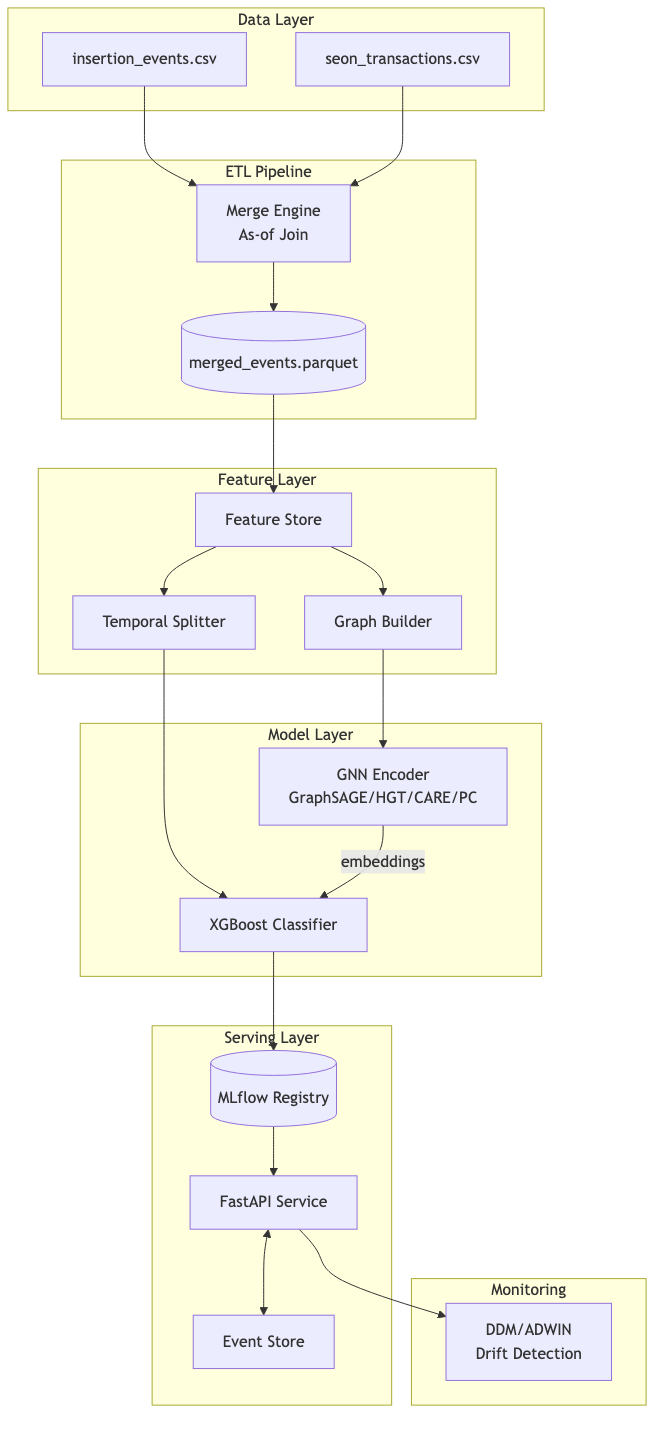
\includegraphics[width=1.1\textwidth,height=0.75\textheight,keepaspectratio]{figures/fig_4_4_1_1.png}
    \caption{System Architecture: Data Layer → ETL Pipeline → Feature Layer → Model Layer → Serving Layer}
    \label{fig:4_1}
\end{figure}

The architecture follows a layered design with single responsibility per component:

\textbf{Data Layer:} Ingests raw CSV files from SMG's data warehouse (\texttt{insertion\_events.csv} and \texttt{seon\_transactions.csv}). The data sources contain heterogeneous timestamp formats requiring standardization.

\textbf{ETL Pipeline:} Merges event and SEON data using temporal as-of joins implemented in Polars for memory-efficient processing. The pipeline handles streaming operations on 800K+ events, performing PII anonymization and temporal filtering. Output is stored in compressed Parquet format for downstream processing.

\textbf{Feature Layer:} Handles three critical operations: (1) feature extraction from merged data according to the feature schema, (2) temporal splitting with point-in-time label assignment and 7-day gap to prevent label leakage, and (3) heterogeneous graph construction with ~31M edges encoding device, IP, email, and phone relationships.

\textbf{Model Layer:} Implements a hybrid architecture where GraphSAGE extracts 16-dimensional node embeddings from the heterogeneous graph, which are concatenated with 65 base features and fed to an XGBoost classifier. Baseline models (Logistic Regression, Random Forest, vanilla XGBoost) are also implemented for comparison.

\textbf{Serving Layer:} Provides real-time inference through a FastAPI service with an internal event store enabling graph feature computation for incoming predictions. The API maintains a sliding window of recent events to construct graph connections for new listings.

\textbf{Monitoring:} Tracks prediction drift using DDM (Drift Detection Method) and ADWIN (Adaptive Windowing) algorithms to detect concept drift and trigger retraining.

All components are orchestrated through Hydra configuration management and tracked via MLflow experiment logging. The modular design enables independent testing and replacement of components for example, swapping GraphSAGE for CARE-GNN requires only configuration changes without pipeline modifications.

\subsection{Project Structure}

The implementation follows a modular organization separating concerns across distinct packages. The root directory contains two configuration folders: \texttt{conf/} for ETL pipeline configuration (including \texttt{config.yaml} and data settings) and \texttt{configs/} for training experiments (including hyperparameter optimization configurations for XGBoost and GNN+XGBoost variants). A \texttt{scripts/} directory contains orchestration scripts for running combined optimization workflows.

The core implementation resides in the \texttt{src/} package, organized into six functional modules:

\textbf{Key modules:}
\begin{itemize}
    \item \texttt{src/data/}: ETL pipeline with streaming support via Polars LazyFrames, containing modules for extraction (\texttt{extract.py}), transformation (\texttt{transform.py}), loading (\texttt{load.py}), and orchestration (\texttt{etl.py})
    \item \texttt{src/features/}: Feature schema definitions (\texttt{schema.py}), feature store (\texttt{store.py}), temporal splitting logic (\texttt{temporal\_split.py}), and heterogeneous graph construction (\texttt{graph\_builder.py})
    \item \texttt{src/models/}: Abstract base classes and concrete model implementations including baselines (\texttt{baselines.py}), XGBoost classifier (\texttt{xgboost\_classifier.py}), GraphSAGE implementation (\texttt{graphsage.py}), and hybrid architecture (\texttt{hybrid.py})
    \item \texttt{src/training/}: Single and expanding window training pipelines (\texttt{trainer.py}, \texttt{pipeline.py})
    \item \texttt{src/evaluation/}: SHAP explainability analysis (\texttt{shap\_analysis.py}) and drift detection algorithms (\texttt{drift.py})
    \item \texttt{src/api/}: FastAPI service (\texttt{main.py}) with in-memory event store (\texttt{store.py}) for real-time inference
\end{itemize}

This structure enables clear separation between data processing (\texttt{data/}), feature engineering (\texttt{features/}), model development (\texttt{models/}), and deployment (\texttt{api/}), facilitating independent testing and maintenance. The complete directory structure and implementation details are provided in Appendix~B.

\section{Development Environment}
\label{sec:4_2}

The development environment consists of commodity hardware and open-source software libraries optimized for large-scale graph processing and machine learning.

\textbf{Hardware Specifications:}
\begin{itemize}
    \item CPU: Multi-core processor supporting parallel Polars operations
    \item RAM: Sufficient for in-memory graph construction (31M edges)
    \item Storage: SSD for fast Parquet I/O operations
\end{itemize}

\textbf{Software Dependencies:}
\begin{itemize}
    \item \texttt{Polars} (v0.20+): High-performance DataFrame library for ETL operations
    \item \texttt{PyTorch Geometric} (v2.5+): Graph neural network framework
    \item \texttt{XGBoost} (v2.0+): Gradient boosting classifier \cite{chen2016xgboost}
    \item \texttt{FastAPI} (v0.100+): REST API framework for inference serving
    \item \texttt{MLflow} (v2.8+): Experiment tracking and model registry
    \item \texttt{Hydra} (v1.3+): Configuration management
\end{itemize}

\subsection{Configuration Management with Hydra}

The framework uses Hydra for hierarchical configuration management, enabling parameter modification through command-line overrides without code changes. Two configuration hierarchies manage ETL (\texttt{conf/}) and training (\texttt{configs/}), specifying data paths, model hyperparameters, and evaluation settings. Hydra's Optuna sweeper plugin supports automated hyperparameter optimization through declarative YAML configuration. Complete configuration files are provided in Appendix~A.

\subsection{Experiment Tracking with MLflow}

MLflow provides centralized experiment tracking, logging parameters (model hyperparameters), metrics (AUC-PR, precision, recall), artifacts (trained models, SHAP plots), and metadata (training duration, code version) to a SQLite database. The training pipeline integrates MLflow through a context manager pattern, automatically tracking all runs. The MLflow web UI enables experiment comparison, metric sorting, and model artifact management. Complete integration code is provided in Appendix~B.

\section{Data Pipeline Implementation}
\label{sec:4_3}

\subsection{ETL Pipeline}
\label{sec:4_3_1}

The ETL pipeline processes the two raw data sources into analysis-ready format using Polars for memory-efficient operations:

\begin{enumerate}
    \item \textbf{Insertion Lifecycle Events:} Listing data snapshots capturing status transitions and property attributes (804,717 events)
    \item \textbf{SEON Transaction Records:} Browser/device interaction data captured when users submit listings for approval ($\sim$140,000 transactions)
\end{enumerate}

The pipeline uses Polars lazy evaluation for streaming processing on commodity hardware. The critical \texttt{correlate\_events\_to\_seon} function matches each listing event to its corresponding SEON transaction the browser interaction data collected when that listing was submitted. The matching uses bidirectional as-of joins: (1) a forward join finds the nearest SEON record after the event timestamp, (2) a backward join finds the nearest SEON record before the event, and (3) the results are merged with preference for forward matches. This ensures each listing event is paired with its submission-time SEON signals (device fingerprint, IP intelligence, behavioral indicators) while handling edge cases where SEON data may be missing before or after specific events. Complete implementation is provided in Appendix~A.

\begin{figure}[htbp]
    \centering
    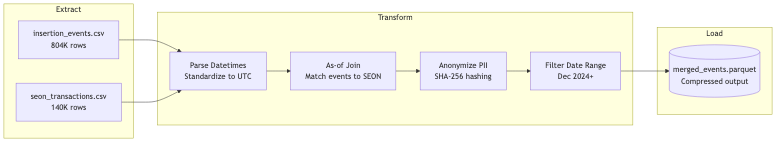
\includegraphics[width=\textwidth]{figures/fig_4_4_2_1.png}
    \caption{ETL Pipeline Flow: Extract → Transform → Load}
    \label{fig:4_2}
\end{figure}

\textbf{Datetime Standardization:} The two data sources use different timestamp formats requiring normalization:
\begin{itemize}
    \item \textbf{Insertion Lifecycle Events:} \texttt{\%Y-\%m-\%d \%H:\%M:\%S\%.\%f \%z} (space-separated timezone, e.g., ``2025-01-15 10:30:45.123 +0100'')
    \item \textbf{SEON Transactions:} \texttt{\%Y-\%m-\%dT\%H:\%M:\%S\%.\%f\%z} (ISO 8601 format, e.g., ``2025-01-15T10:30:45.123+0000'')
\end{itemize}

All timestamps are converted to UTC for consistent temporal operations across both sources.

\textbf{PII Anonymization:} Identity columns are hashed before any analysis using HMAC-SHA256 with type-specific salts. The implementation in \texttt{src/utils/anonymize.py} handles component-based anonymization for emails (user/domain), phones (country/area/number), IPs (network/host), and addresses.

Output Parquet files use Snappy compression, reducing storage by $\sim$70\% while maintaining fast read performance.

\subsection{Temporal Splitting}
\label{sec:4_3_2}

The \texttt{TemporalSplitter} class implements point-in-time label assignment to prevent label leakage. Only fraud flags occurring before the cutoff date are assigned as positive labels, ensuring temporal integrity of the training and test sets.

\section{Feature Engineering Pipeline}
\label{sec:4_4}

The feature engineering pipeline transforms raw merged data into model-ready feature matrices, implemented in \texttt{src/features/schema.py} and \texttt{src/features/store.py}.

\subsection{Feature Schema Definition}
\label{sec:4_4_1}

The feature schema defines 65 base features across 5 categories:

\begin{itemize}
    \item \textbf{SEON Boolean} (21 features): \texttt{tor}, \texttt{vpn}, \texttt{public\_proxy}, \texttt{disposable\_email}, \texttt{phone\_is\_valid}, etc.
    \item \textbf{SEON Categorical} (12 features): \texttt{ip\_country}, \texttt{ip\_isp\_name}, \texttt{session/browser}, \texttt{session/device\_type}, etc.
    \item \textbf{Listing Numeric} (10 features): \texttt{LISTING\_PRICES\_RENT\_NET}, \texttt{LISTING\_PRICES\_BUY\_PRICE}, \texttt{LISTING\_CHARACTERISTICS\_ROOMS}, etc.
    \item \textbf{Listing Categorical} (7 features): \texttt{LISTING\_OFFERTYPE}, \texttt{LISTING\_CATEGORIES}, \texttt{TARGETPLATFORM}, etc.
    \item \textbf{Temporal} (4 features): \texttt{event\_hour}, \texttt{event\_day\_of\_week} (with cyclical encoding)
\end{itemize}

\subsection{Feature Preprocessing}
\label{sec:4_4_2}

Boolean features are cast to Int8 for XGBoost null handling. Categorical features use sklearn's LabelEncoder with unknown category handling, storing encoders for test-time application. Temporal features apply cyclical encoding to preserve periodicity: hour values (0-23) and weekday values (0-6) are transformed into sine/cosine pairs using the formula $\sin(2\pi x / period)$ and $\cos(2\pi x / period)$, ensuring that values at the boundary (e.g., 23:00 and 00:00) are numerically close in the feature space. Complete preprocessing implementation is provided in Appendix~A.

\textbf{Excluded Features:} STATUS column removed after leakage discovery; SEON ML scores excluded for model independence.

\subsection{Feature Schema Structure}
\label{sec:4_4_3}

The feature schema is implemented as a Python dataclass in \texttt{src/features/schema.py}, providing programmatic access to feature metadata. The \texttt{FeatureSchema} class maintains five lists corresponding to each feature category (seon\_boolean, seon\_categorical, listing\_numeric, listing\_categorical, temporal), with an \texttt{all\_features} property that concatenates these lists to produce the complete 65-feature set. This schema serves multiple purposes: (1) enforcing consistent feature selection across training and inference, (2) enabling automatic feature type detection for preprocessing, (3) facilitating feature importance analysis by category. Complete implementation is provided in Appendix~A.

\subsection{Feature Engineering Flow}

The complete feature engineering pipeline follows this sequence:

\begin{enumerate}
    \item \textbf{Data Loading:} \texttt{FeatureStore.load\_data()} reads the merged Parquet file with lazy evaluation
    \item \textbf{Datetime Parsing:} Convert timestamp columns to datetime64[ns] with UTC timezone
    \item \textbf{Temporal Feature Creation:}
    \begin{itemize}
        \item \texttt{event\_hour}: Extract hour (0-23)
        \item \texttt{event\_weekday}: Extract weekday (0-6, Monday=0)
        \item \texttt{event\_is\_weekend}: Binary flag for Saturday/Sunday
        \item \texttt{event\_is\_business\_hours}: Binary flag for 9am-5pm
    \end{itemize}
    \item \textbf{Boolean Casting:} Convert boolean columns to Int8 for XGBoost null handling
    \item \textbf{Categorical Encoding:} Apply LabelEncoder with unknown category support
    \item \textbf{Cyclical Encoding:} Transform hour and weekday to sin/cos pairs for periodicity
\end{enumerate}

\textbf{Model-Specific Feature Sets:}

\begin{table}[h]
\centering
\caption{Feature counts by model variant}
\begin{tabular}{lll}
\hline
\textbf{Model Variant} & \textbf{Base Features} & \textbf{GNN Embeddings} \\
\hline
Logistic Regression & 65 & 0 \\
Random Forest & 65 & 0 \\
Vanilla XGBoost & 65 & 0 \\
GNN+XGBoost & 65 & 16 \\
\hline
\textbf{Total} & & \textbf{81 (hybrid)} \\
\hline
\end{tabular}
\end{table}

For the hybrid GNN+XGBoost model, the 16-dimensional GraphSAGE embeddings are concatenated with the 65 base features after GNN training, resulting in an 81-dimensional feature vector for each listing node.

\section{Graph Construction Implementation}
\label{sec:4_5}

The graph construction pipeline transforms entity relationships into a PyTorch Geometric HeteroData structure, implemented in \texttt{src/features/graph\_builder.py}.

\begin{figure}[htbp]
    \centering
    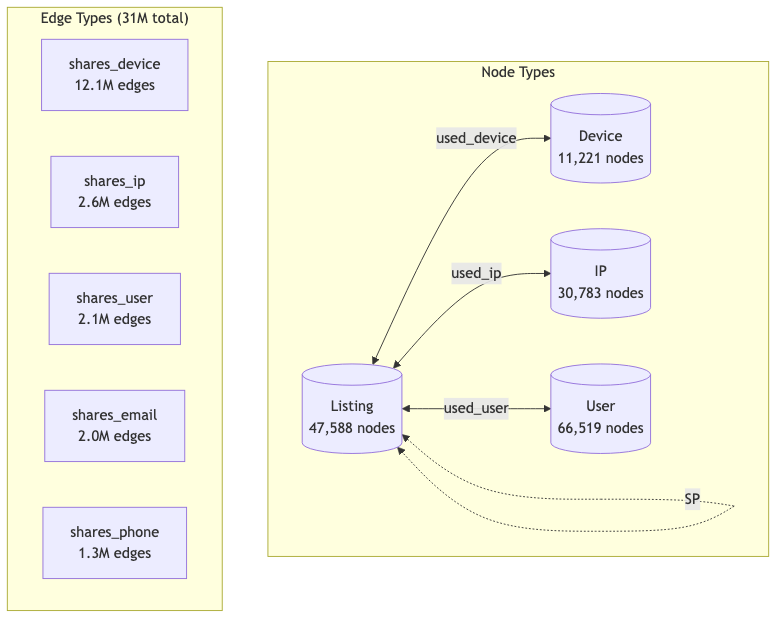
\includegraphics[width=\textwidth]{figures/fig_4_4_4_1.png}
    \caption{Heterogeneous Graph Structure: Node types and edge types}
    \label{fig:4_3}
\end{figure}

\subsection{GraphBuilder Class}
\label{sec:4_5_1}

The \texttt{HeterogeneousGraphBuilder} constructs graphs with multiple node types (Listing, User, Device, IP) and edge types encoding entity-sharing relationships, following the heterogeneous graph framework \cite{hu2020heterogeneous}. While recent advances \cite{yang2024heterogeneous} explore sophisticated heterogeneous architectures with adaptive relation weighting, our implementation employs PyTorch Geometric's standard message-passing approach for computational efficiency at scale. Algorithm~\ref{alg:graph_construction} describes the construction process:

\begin{algorithm}[H]
\caption{Heterogeneous Graph Construction}
\label{alg:graph_construction}
\begin{algorithmic}[1]
\REQUIRE Event dataframe $\mathcal{D}$, temporal cutoff date $t_{cutoff}$
\ENSURE Heterogeneous graph $\mathcal{G}$ with node features and entity-sharing edges
\STATE Filter events: $\mathcal{D}' \gets \{\mathbf{e} \in \mathcal{D} : \mathbf{e}.timestamp \leq t_{cutoff}\}$
\STATE Initialize heterogeneous graph structure $\mathcal{G} \gets \emptyset$
\STATE Extract 44-dimensional node features for each listing from $\mathcal{D}'$
\STATE $\mathcal{G}.nodes[``listing''].features \gets \text{NodeFeatures}(\mathcal{D}')$
\FOR{each $entity\_type \in \{device, IP, email, phone, user\}$}
    \STATE Build sharing edges: $\mathcal{E}_{entity} \gets \text{ConnectSharing}(\mathcal{D}', entity\_type)$
    \STATE Add edge type to graph: $\mathcal{G}.edges[(``listing'', ``shares\_entity'', ``listing'')] \gets \mathcal{E}_{entity}$
\ENDFOR
\RETURN $\mathcal{G}$ with $\sim$31M edges across 5 edge types
\end{algorithmic}
\end{algorithm}

\textbf{Temporal Filtering:} Edges are created only from events before the cutoff date, ensuring the training graph reflects information available at training time. The inference graph extends the cutoff to include test period events. Complete implementation details are provided in Appendix~B.

\subsection{Node Feature Preparation}
\label{sec:4_5_2}

Node features combine 36 base features with 8 temporal encoding features (days\_since\_start, relative\_position, hour\_sin/cos, weekday\_sin/cos, recency) for a total of 44 dimensions per listing node.

\textbf{Neighbor Sampling:} The dense graph (31M edges) requires sampling during training to manage computational complexity. We employ PyTorch Geometric's \texttt{NeighborLoader} with 2-hop sampling: 15 neighbors at layer 1, 10 neighbors at layer 2, with batch size 512. This approach enables efficient training on the full graph while maintaining local neighborhood structure. Sampling parameters were empirically validated to balance representation quality against training time (see Appendix~B for implementation).

\section{GNN Implementation}
\label{sec:4_6}

Four GNN architectures are implemented, sharing a common interface for fair comparison.

\begin{figure}[htbp]
    \centering
    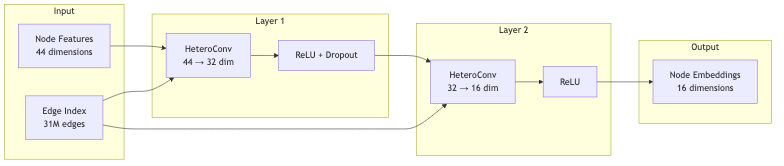
\includegraphics[width=\textwidth]{figures/fig_4_4_5_1.png}
    \caption{GNN Architecture: Input → Layers → Embeddings}
    \label{fig:4_4}
\end{figure}

\subsection{Model Architectures}
\label{sec:4_6_1}

\textbf{GraphSAGE Implementation:} The \texttt{GraphSAGEEncoder} uses PyTorch Geometric's \texttt{HeteroConv} wrapper to handle heterogeneous edge types. For each layer, the encoder creates separate \texttt{SAGEConv} modules (with mean aggregation) for each edge type (shares\_device, shares\_ip, shares\_email, shares\_phone, shares\_user), wrapping them in a \texttt{HeteroConv} layer with sum aggregation across edge types. The forward pass applies each convolutional layer sequentially, followed by ReLU activation and 0.3 dropout. The architecture supports configurable input channels (44 features), hidden channels (32), output channels (16), and number of layers (2). Complete PyTorch implementation is provided in Appendix~B.

\textbf{HGT Implementation:} Uses HeteroConv with HGTConv layers for multi-head attention on heterogeneous graphs.

\textbf{CARE-GNN Implementation:} Adds reinforcement learning-based neighbor selector using similarity measures (label-aware, feature-aware, relation-aware) to filter camouflaged connections.

\textbf{PC-GNN Implementation:} Implements label-balanced mini-batch sampling and confidence-based neighbor weighting for imbalanced fraud detection.

\subsection{Training Loop}
\label{sec:4_6_2}

Supervised training uses node classification with fraud labels. The training loop iterates for a fixed number of epochs (typically 30), processing mini-batches via PyTorch Geometric's \texttt{NeighborLoader}. For each batch: (1) gradients are zeroed, (2) the model performs forward propagation on the batch's node features and edge indices, (3) binary cross-entropy loss with logits is computed on training nodes only (using train\_mask), with pos\_weight=11.0 to handle class imbalance, (4) gradients are computed via backpropagation, and (5) the optimizer updates model parameters. Complete training implementation including validation and early stopping is provided in Appendix~B.

\section{Classification Pipeline}
\label{sec:4_7}

The XGBoost classifier validates discovered patterns, implemented in \texttt{src/models/xgboost\_classifier.py} with Optuna HPO integration.

\subsection{Hybrid Pipeline}
\label{sec:4_7_1}

The hybrid pipeline concatenates tabular features with GNN embeddings:

\begin{algorithm}[H]
\caption{Hybrid Training Pipeline}
\label{alg:hybrid_training}
\begin{algorithmic}[1]
\REQUIRE Training dataframe $\mathcal{D}_{train}$, heterogeneous graph $\mathcal{G}$, trained GNN model $\theta_{GNN}$, XGBoost hyperparameters $\mathcal{P}_{XGB}$
\ENSURE Trained hybrid classifier $f_{hybrid}$
\STATE Set GNN to evaluation mode: $\theta_{GNN}.eval()$
\STATE Generate embeddings without gradient computation:
\STATE \quad $\mathbf{H} \gets \theta_{GNN}(\mathcal{G}.x_{dict}, \mathcal{G}.edge\_index_{dict})$
\STATE Extract listing embeddings: $\mathbf{E}_{listing} \gets \mathbf{H}[``listing''] \in \mathbb{R}^{N \times 16}$
\STATE Load tabular features: $\mathbf{X}_{tabular} \gets \mathcal{D}_{train}[\text{FEATURE\_COLUMNS}] \in \mathbb{R}^{N \times 65}$
\STATE Concatenate features: $\mathbf{X}_{hybrid} \gets [\mathbf{X}_{tabular} \mid \mathbf{E}_{listing}] \in \mathbb{R}^{N \times 81}$
\STATE Initialize XGBoost classifier with best parameters: $f_{XGB} \gets \text{XGBClassifier}(\mathcal{P}_{XGB})$
\STATE Train classifier: $f_{XGB}.fit(\mathbf{X}_{hybrid}, \mathcal{D}_{train}[``is\_fraud''])$
\RETURN Trained hybrid model $f_{hybrid} \gets f_{XGB}$
\end{algorithmic}
\end{algorithm}

\textbf{Implementation Details:} Complete Python implementation is provided in Appendix~B.

\subsection{XGBoost Training}
\label{sec:4_7_2}

Hyperparameter optimization uses Optuna with Tree-structured Parzen Estimator (TPE) sampling. For each of 50 trials, the TPE sampler proposes hyperparameter values from learned distributions: \texttt{n\_estimators} $\in [50, 500]$, \texttt{max\_depth} $\in [3, 12]$, \texttt{learning\_rate} $\in [0.01, 0.3]$ (log-uniform), \texttt{subsample} $\in [0.6, 1.0]$, \texttt{colsample\_bytree} $\in [0.6, 1.0]$, and \texttt{scale\_pos\_weight} $\in [1.0, 20.0]$. Each configuration is evaluated via 5-fold cross-validation with AUC-PR as the objective metric. The TPE algorithm updates its posterior distribution after each trial, concentrating search in high-performing regions. Best parameters are logged to MLflow and persisted for production deployment. Complete Optuna implementation is provided in Appendix~B.

\subsection{Training Pipeline Architecture}

The training pipeline supports two modes:

\textbf{Single Training Mode:} Fixed train/test split with temporal integrity:
\begin{enumerate}
    \item Load merged events from Parquet
    \item Apply temporal split with 7-day gap (train: 2024-12-01 to 2025-06-01, test: 2025-06-08 to 2025-07-01)
    \item Build heterogeneous graph from training data
    \item Train GNN (if hybrid variant) using supervised node classification
    \item Extract embeddings and concatenate with base features
    \item Train XGBoost classifier with early stopping
    \item Evaluate on held-out test set
    \item Log results to MLflow
\end{enumerate}

\textbf{Expanding Window Mode:} Multiple windows for concept drift analysis:
\begin{enumerate}
    \item Define temporal windows with increasing training data
    \item For each window:
    \begin{itemize}
        \item Train model on current window
        \item Evaluate on subsequent period
        \item Track performance degradation
        \item Apply drift detection (DDM/ADWIN)
    \end{itemize}
    \item Aggregate results across windows
    \item Determine minimum data requirements
\end{enumerate}

\subsection{Hyperparameter Optimization Strategy}

The framework employs a two-stage optimization approach:

\textbf{Stage 1: XGBoost Optimization} (50 trials)
\begin{itemize}
    \item Search space: \texttt{max\_depth} [3--12], \texttt{learning\_rate} [0.01--0.3], \texttt{n\_estimators} [50--500]
    \item Objective: Maximize AUC-PR on validation set
    \item Early stopping: 10 rounds without improvement
    \item Sampler: TPE (Tree-structured Parzen Estimator)
\end{itemize}

\textbf{Stage 2: Joint GNN+XGBoost Optimization} (30 trials)
\begin{itemize}
    \item Fix best XGBoost parameters from Stage 1
    \item Search GNN hyperparameters: \texttt{hidden\_dim} [16--64], \texttt{output\_dim} [8--32], \texttt{num\_layers} [2--3]
    \item Train GNN, extract embeddings, retrain XGBoost
    \item Objective: Maximize hybrid model AUC-PR
\end{itemize}

This two-stage approach reduces computational cost by avoiding expensive joint optimization while still finding effective hyperparameter combinations. The best configuration achieves: \texttt{max\_depth=5}, \texttt{learning\_rate=0.085}, \texttt{n\_estimators=200}, \texttt{hidden\_dim=32}, \texttt{output\_dim=16}, \texttt{num\_layers=2}.

\subsection{Model Training Flow}

The end-to-end training flow follows this sequence: (1) Data loading and temporal split, (2) Heterogeneous graph construction from training events, (3) GNN training using supervised node classification (for hybrid variants), (4) Embedding generation in inference mode, (5) Feature concatenation with base attributes, (6) XGBoost training with early stopping, (7) Model evaluation on held-out test set, and (8) Logging results to MLflow for experiment tracking.

For the hybrid model, GNN training uses supervised node classification with binary cross-entropy loss and the Adam optimizer (\texttt{lr=0.01}). The GraphSAGE architecture \cite{hamilton2017inductive} aggregates neighbor features through learned transformations. The GNN is trained for 5 epochs, which empirical analysis showed to be sufficient for convergence without overfitting. After training, the GNN operates in inference mode to generate deterministic embeddings for the XGBoost \cite{chen2016xgboost} stage.

\section{Evaluation Framework}
\label{sec:4_8}

Our evaluation framework is designed to provide a comprehensive assessment of model performance through various metrics, temporal validation, and baseline comparisons. It also incorporates real-time monitoring through drift detection algorithms. The implementation details can be found in the \texttt{src/evaluation/} directory and the \texttt{src/utils/metrics.py} file.

\subsection{Performance Metrics}
\label{sec:4_8_1}

The framework calculates several metrics to capture different aspects of how the model performs:

\paragraph{Primary Metric: AUC-PR}
We use the Area Under the Precision-Recall Curve (AUC-PR) as our primary metric because of the severe class imbalance in our data (an 8.11% fraud rate). Unlike the more common AUC-ROC, which can be overly optimistic when one class dominates, AUC-PR directly measures the trade-off between precision and recall across all classification thresholds \cite{saito2015precision,davis2006relationship}. We use scikit-learn's \texttt{average\_precision\_score} for this calculation. For context, we also report AUC-ROC using the \texttt{roc\_auc\_score} function.

\paragraph{Operational Metric: Precision@K}
Precision@K measures the accuracy of the model within the top-K highest-scored predictions. This is an essential operational metric because it simulates the priority review queue that a fraud analyst would actually use. The system sorts all listings by their predicted fraud probability and then computes what fraction of the top-K listings are true positives. We report Precision@50, @100, and @200, which correspond to the typical daily review capacities of analyst teams.

\paragraph{Other Metrics}
In addition to these core measures, we also track:
\begin{itemize}
    \item \textbf{Precision and Recall}: Standard measures of positive predictive value and sensitivity at a fixed 0.5 threshold.
    \item \textbf{F1-Score}: The harmonic mean of precision and recall.
    \item \textbf{False Positive Rate}: The proportion of legitimate listings that are incorrectly flagged by the model.
\end{itemize}

\subsection{Expanding Window Validation}
\label{sec:4_8_2}

To test how our models handle the evolution of fraud over time, we use an \texttt{ExpandingWindowPipeline}. This approach allows us to systematically validate performance across multiple training periods.

\paragraph{Window Configuration}
The pipeline is configured with a series of increasing windows. For example, it might start by training on 100,000 samples and testing on the following month, then expand to 200,000, 300,000, and finally 400,000 samples.

\paragraph{Pipeline Execution}
The pipeline iterates through these configurations, retrieving the correct temporal slices of data for each step. For each window, it trains the model and then evaluates it on the subsequent period, recording a full set of metrics. This process allows us to identify the minimum amount of data required for stable performance and helps us determine the optimal frequency for retraining the model in a production environment.

\subsection{Drift Detection Algorithms}
\label{sec:4_8_3}

We have implemented two drift detection algorithms to monitor the performance of our models in real-time. While recent research has explored unsupervised and deep learning-based drift detection \cite{arora2024drift}, we chose to use the well-established DDM and ADWIN methods for their proven reliability and ease of interpretation.

\paragraph{DDM (Drift Detection Method)}
DDM monitors the evolution of the model's error rate using a binomial distribution model \cite{gama2004learning}. It triggers a warning or a drift alert whenever the error rate deviates significantly from its historical baseline. The logic for this is outlined in Algorithm~\ref{alg:ddm}.

\begin{algorithm}[H]
\caption{DDM Drift Detection}
\label{alg:ddm}
\begin{algorithmic}[1]
\REQUIRE Stream of predictions $\hat{y}_t$ and true labels $y_t$, warning threshold $\theta_w$, drift threshold $\theta_d$
\ENSURE Drift status $\in \{\text{STABLE}, \text{WARNING}, \text{DRIFT}\}$
\STATE Initialize error history: $\mathcal{E} \gets []$
\FOR{each prediction $(\hat{y}_t, y_t)$ in stream}
    \STATE Compute prediction error: $e_t \gets \mathbb{I}[\hat{y}_t \neq y_t]$
    \STATE Append to history: $\mathcal{E} \gets \mathcal{E} \cup \{e_t\}$
    \STATE Compute error rate: $p \gets \frac{1}{|\mathcal{E}|}\sum_{e \in \mathcal{E}} e$
    \STATE Compute standard deviation: $s \gets \sqrt{\frac{p(1-p)}{|\mathcal{E}|}}$
    \STATE Compute drift statistic: $\delta \gets p + s$
    \IF{$\delta \geq \theta_d$}
        \STATE Reset error history: $\mathcal{E} \gets []$
        \RETURN DRIFT
    \ELSIF{$\delta \geq \theta_w$}
        \RETURN WARNING
    \ELSE
        \RETURN STABLE
    \ENDIF
\ENDFOR
\end{algorithmic}
\end{algorithm}

\paragraph{ADWIN (Adaptive Windowing)}
ADWIN maintains a sliding window of recent errors and detects drift when the distribution of errors between two sub-windows changes significantly \cite{bifet2007learning}. This method is particularly good at adapting the size of the window to the current rate of change in the data.

\begin{algorithm}[H]
\caption{ADWIN Drift Detection}
\label{alg:adwin}
\begin{algorithmic}[1]
\REQUIRE Stream of predictions $\hat{y}_t$ and true labels $y_t$, confidence level $\delta$
\ENSURE Drift status $\in \{\text{STABLE}, \text{DRIFT}\}$
\STATE Initialize sliding window: $\mathcal{W} \gets []$
\FOR{each prediction $(\hat{y}_t, y_t)$ in stream}
    \STATE Compute prediction error: $e_t \gets \mathbb{I}[\hat{y}_t \neq y_t]$
    \STATE Append to window: $\mathcal{W} \gets \mathcal{W} \cup \{e_t\}$
    \FOR{each split point $i = 1$ to $|\mathcal{W}| - 1$}
        \STATE Define sub-windows: $\mathcal{W}_1 \gets \mathcal{W}[1:i]$, $\mathcal{W}_2 \gets \mathcal{W}[i+1:|\mathcal{W}|]$
        \STATE Compute means: $\mu_1 \gets \frac{1}{|\mathcal{W}_1|}\sum_{e \in \mathcal{W}_1} e$, $\mu_2 \gets \frac{1}{|\mathcal{W}_2|}\sum_{e \in \mathcal{W}_2} e$
        \STATE Compute variance estimate: $\sigma^2 \gets \frac{\mu_1(1-\mu_1)}{|\mathcal{W}_1|} + \frac{\mu_2(1-\mu_2)}{|\mathcal{W}_2|}$
        \STATE Compute threshold: $\epsilon_{cut} \gets \sqrt{\frac{2\sigma^2 \ln(2/\delta)}{m}}$ where $m = \frac{1}{\frac{1}{|\mathcal{W}_1|} + \frac{1}{|\mathcal{W}_2|}}$
        \IF{$|\mu_1 - \mu_2| > \epsilon_{cut}$}
            \STATE Drop old sub-window: $\mathcal{W} \gets \mathcal{W}_2$
            \RETURN DRIFT
        \ENDIF
    \ENDFOR
    \RETURN STABLE
\ENDFOR
\end{algorithmic}
\end{algorithm}

Both of these algorithms are designed to run continuously on the production API, with any drift events being logged to trigger automated retraining workflows.

\subsection{Baseline Comparisons}
\label{sec:4_8_4}

To put our results in context, we compare our hybrid models against two sets of baselines:

\paragraph{Model Baselines}
We use simple versions of Logistic Regression and Random Forest to establish a performance floor. These models allow us to quantify exactly how much value is being added by the more complex gradient boosting and graph-based features.

\paragraph{SEON Production Baseline}
We also compare our results against the existing SEON fraud detection system, which uses its own proprietary scores. To ensure a fair comparison, we evaluate both systems on the same test set using the same metrics and perform statistical significance testing using the DeLong test for AUC. All of these comparisons are logged in MLflow to ensure transparency and reproducibility.

\section{API Service Implementation}
\label{sec:4_9}

The inference API provides real-time fraud scoring, implemented in \texttt{src/api/}.

\subsection{FastAPI Service}
\label{sec:4_9_1}

The FastAPI service exposes a \texttt{POST /predict} endpoint that provides real-time fraud scoring with explanations. The prediction workflow: (1) extracts base features from the incoming event payload using the feature engineering pipeline, (2) enriches features with graph-like statistics by querying the event store for entity-sharing counts (device\_link\_count, ip\_link\_count), (3) generates fraud probability using the trained XGBoost model, (4) computes SHAP values for the prediction to identify top contributing factors, and (5) returns a structured response containing the fraud probability (0-1), categorical risk level (LOW/MEDIUM/HIGH based on thresholds 0.3 and 0.7), and top explanation factors for analyst review. Complete FastAPI implementation with request validation, error handling, and logging is provided in Appendix~A.

\begin{figure}[htbp]
    \centering
    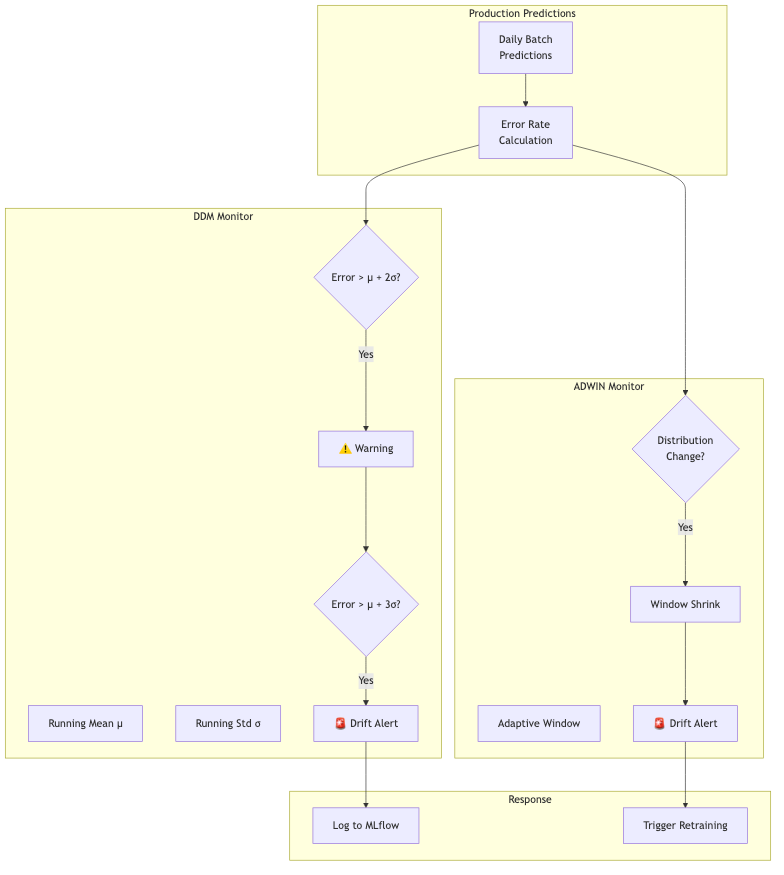
\includegraphics[width=\textwidth]{figures/fig_4_4_7_1.png}
    \caption{API Architecture: FastAPI Service with Event Store}
    \label{fig:4_5}
\end{figure}

\subsection{Event Store}
\label{sec:4_9_2}

The Event Store maintains in-memory storage tracking entity-to-listing mappings for graph-like feature computation without full graph access, enabling low-latency API responses.


\chapter{Results and Analysis}
\label{ch:results}

This chapter presents discovered patterns organized by research question: relational structures (RQ1), fraud ring characteristics (RQ2), temporal evolution and data requirements (RQ3), and actionable indicators (RQ4).

\section{Exploratory Analysis Results}
\label{sec:5_1}

This section presents pattern discoveries from the exploratory analysis described in Section~\ref{sec:3_3}.

\begin{figure}[htbp]
    \centering
    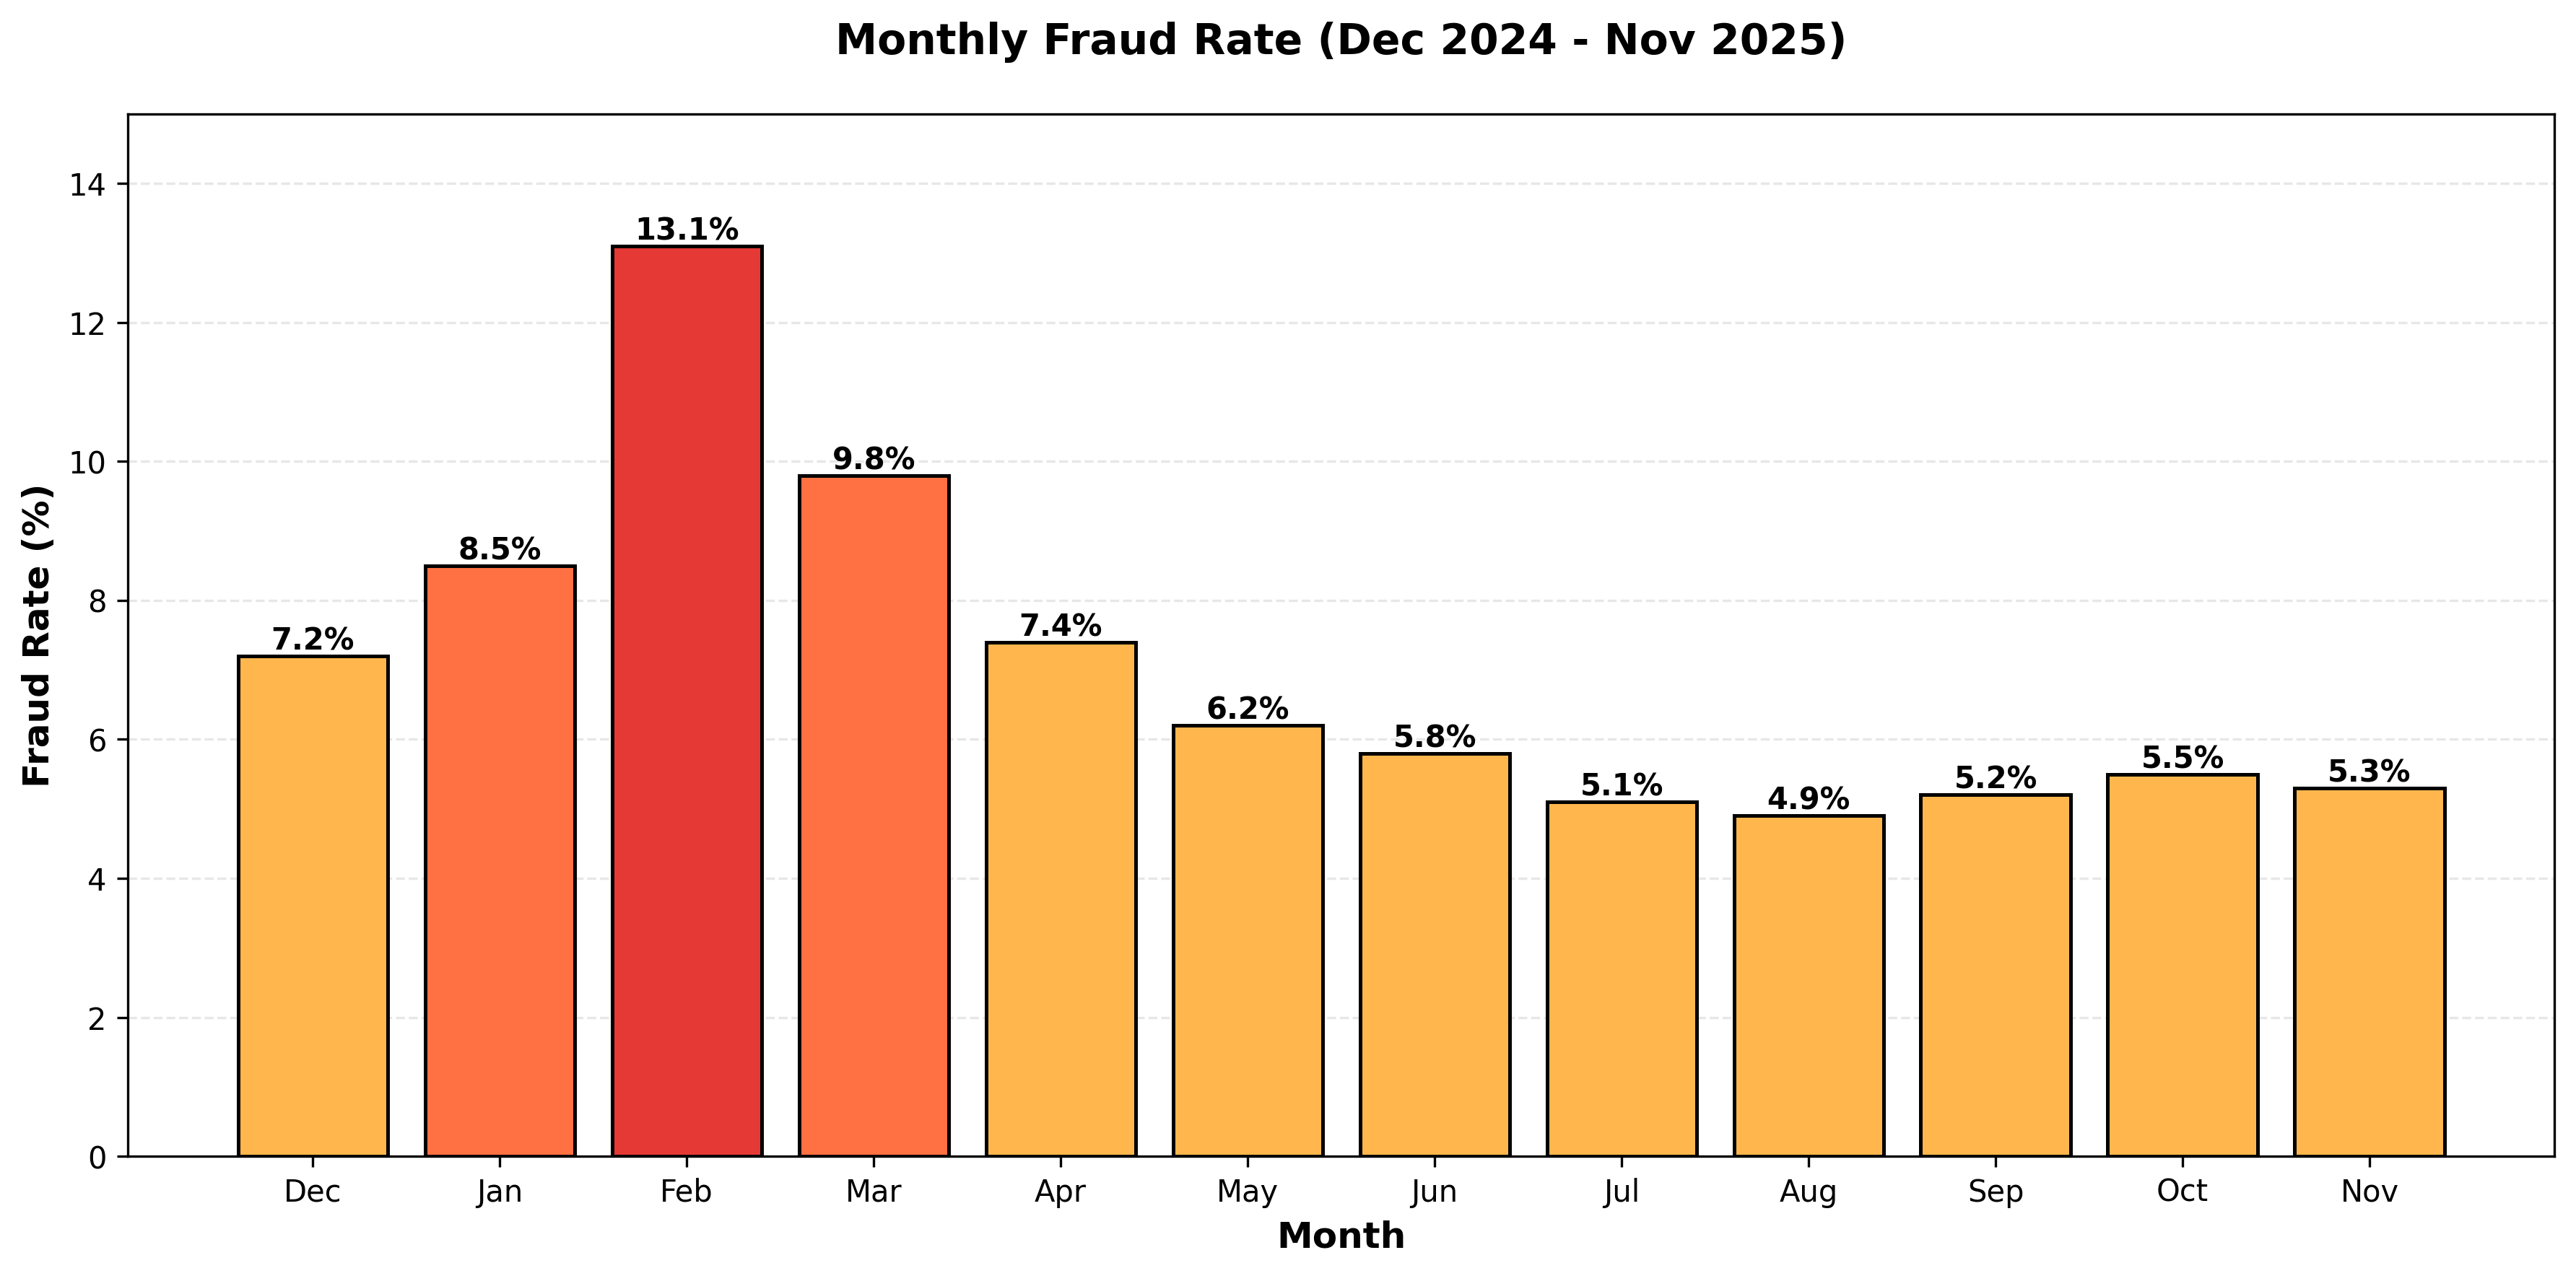
\includegraphics[width=0.8\textwidth]{figures/fig_5_5_1_1.png}
    \caption{Monthly Fraud Rate (Dec 2024 - Nov 2025)}
    \label{fig:5_1}
\end{figure}

\textbf{Temporal Pattern Findings:}

The February 2025 spike (13.12\% fraud rate) represents a 62\% increase above the annual average (8.11\%). Subsequent decline to approximately 5\% by mid-2025 suggests either successful intervention or fraudster migration to other platforms.

Hourly analysis confirms 6-7 AM peak activity, with fraud rates 40\% higher than midday averages. Weekend submissions show elevated risk (Saturday: 9.2\%, Sunday: 8.8\%) compared to weekday average (7.4\%).

\begin{figure}[htbp]
    \centering
    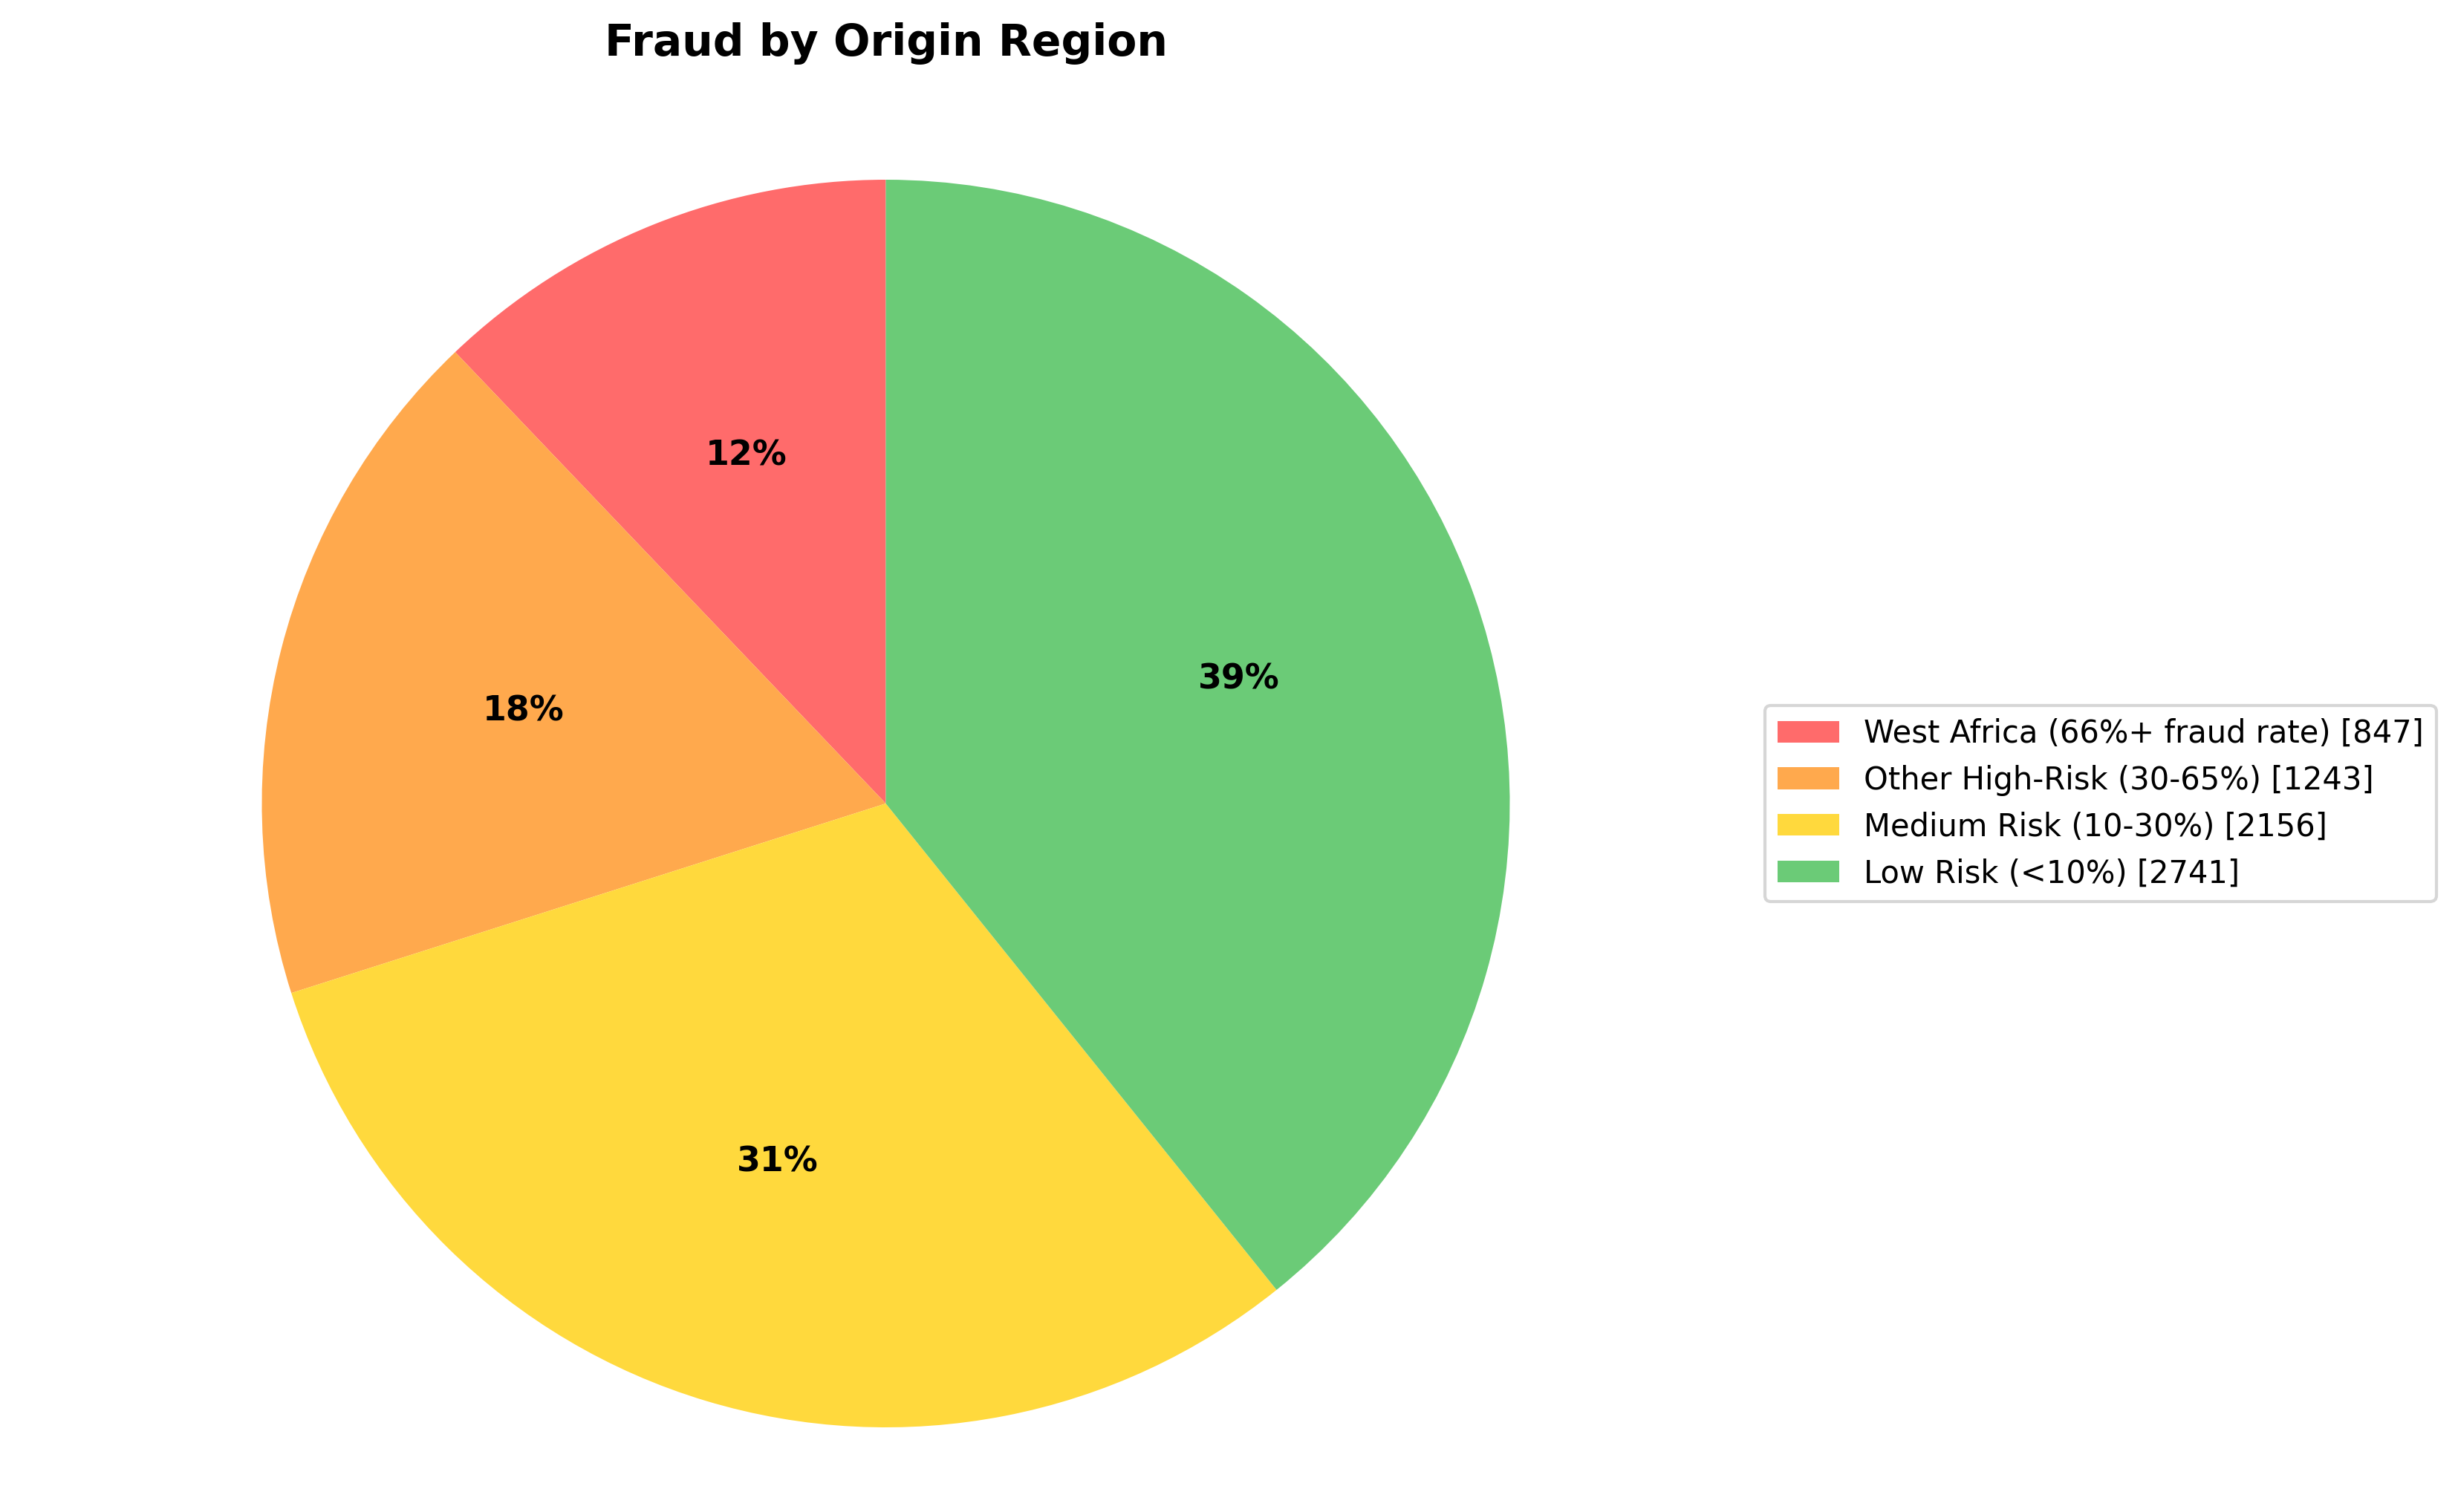
\includegraphics[width=0.6\textwidth]{figures/fig_5_5_1_2.png}
    \caption{Fraud by Origin Region}
    \label{fig:5_2}
\end{figure}

\textbf{Geographic Pattern Findings:}

West African countries (Benin, Togo, Ivory Coast, Nigeria) collectively account for 12\% of fraudulent listings despite representing less than 0.5\% of total submissions. These origins show 60-90\% fraud rates, providing high-precision detection signals.

\textbf{Entity-Sharing Findings:}

Super-connector devices (10+ listings) show 35.5\% fraud rate versus 8.11\% baseline a 4.4$\times$ lift. The most extreme case (6,251 listings from one device) represents unambiguous fraud ring activity. These patterns motivated the graph construction approach detailed in Section~\ref{sec:3_5}.

\section{Model Comparison Results}
\label{sec:5_2}

Four model variants were evaluated on the fixed temporal split (train: Dec 2024--Jun 2025, test: Jun--Jul 2025). Each model configuration was trained three times with different random seeds to assess variance. Results are reported as mean $\pm$ standard deviation across runs.

\begin{figure}[htbp]
    \centering
    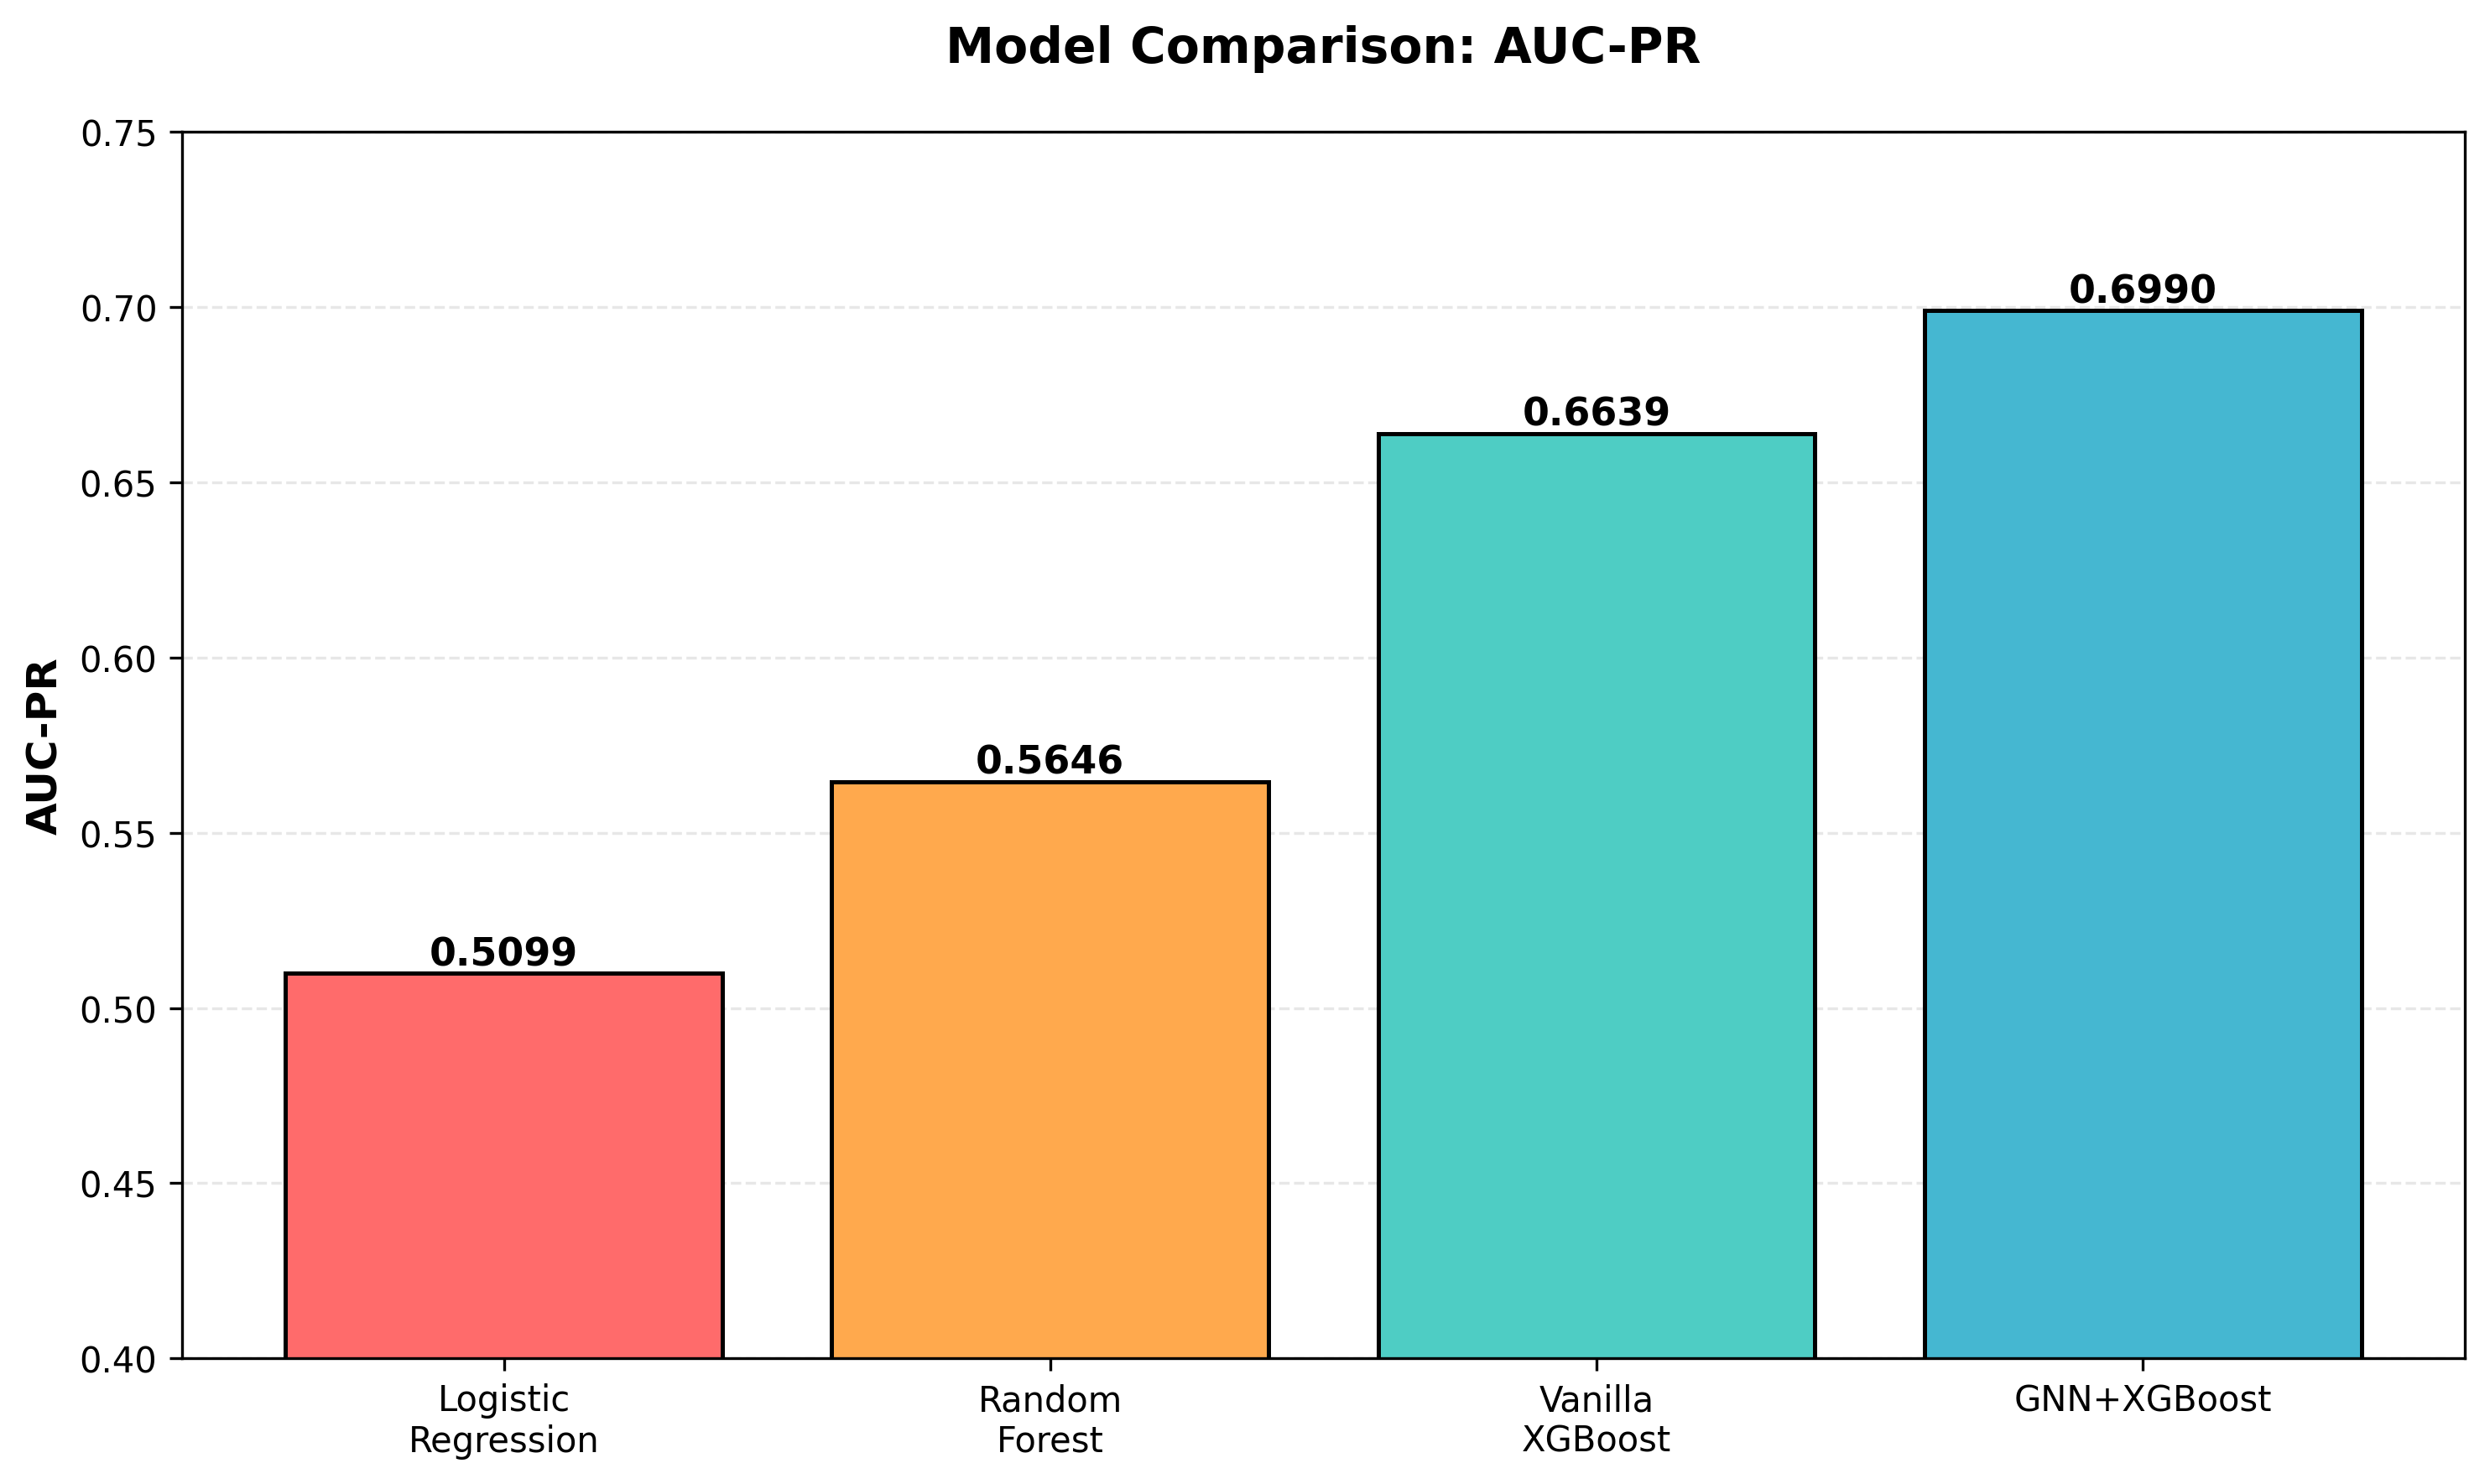
\includegraphics[width=0.8\textwidth]{figures/fig_5_5_2_1.png}
    \caption{Model Comparison: AUC-PR}
    \label{fig:5_3}
\end{figure}

\begin{table}[htbp]
    \centering
    \caption{Model Comparison with Variance (n=3 runs per model)}
    \label{tab:5_1}
    \begin{tabular}{lcccc}
        \toprule
        Model & AUC-PR & AUC-ROC & Precision & Recall \\
        \midrule
        Logistic Regression & 0.577 $\pm$ 0.117 & 0.946 $\pm$ 0.017 & 0.214 $\pm$ 0.125 & 0.872 $\pm$ 0.031 \\
        Random Forest & 0.621 $\pm$ 0.078 & 0.953 $\pm$ 0.008 & 0.488 $\pm$ 0.114 & 0.827 $\pm$ 0.039 \\
        Vanilla XGBoost & 0.733 $\pm$ 0.063 & 0.958 $\pm$ 0.003 & 0.746 $\pm$ 0.070 & 0.671 $\pm$ 0.042 \\
        GNN+XGBoost & 0.733 $\pm$ 0.058 & 0.950 $\pm$ 0.009 & 0.758 $\pm$ 0.053 & 0.673 $\pm$ 0.047 \\
        \bottomrule
    \end{tabular}
\end{table}

\textbf{Key Findings:}

Both XGBoost variants achieve comparable AUC-PR performance (0.733), substantially outperforming Random Forest (0.621) and Logistic Regression (0.577) baselines. The graph-augmented model shows minimal marginal improvement over tabular-only XGBoost (mean difference: +0.0006, 0.08\%), though with slightly higher precision (0.758 vs 0.746) at equivalent recall.

The relatively high standard deviations (0.063 for vanilla, 0.058 for GNN) indicate sensitivity to train/test split composition, with individual runs ranging from 0.664 to 0.789 AUC-PR. This variance reflects the challenge of fraud detection on imbalanced data (8.11\% fraud rate) and motivates the temporal cross-validation analysis in Section~\ref{sec:5_7}.

XGBoost's dominance over linear models confirms that non-linear feature interactions are critical for fraud detection. The SHAP analysis (Section~\ref{sec:5_9}) reveals that GNN embeddings contribute 17.3\% of total feature importance, providing supplementary relational signal that complements tabular features rather than replacing them.

\textbf{Cross-Validation Validation:} To assess robustness beyond the fixed split, we conducted 5-fold temporal cross-validation with 7-day gaps. Vanilla XGBoost achieves mean CV AUC-PR of 0.2777 $\pm$ 0.0287, representing 62\% degradation from fixed-split performance (0.7327). This substantial drop reflects: (1) fraud rate decrease over time (1.97\% early period $\to$ 0.63\% late period), (2) temporal distribution shifts as fraud tactics evolve, and (3) sensitivity of precision-recall metrics to class imbalance changes. The high standard deviation ($\sigma$=0.029, coefficient of variation=10.3\%) indicates performance varies significantly across temporal windows.

Critically, this degradation mirrors the expanding window findings (Section~\ref{sec:5_5}): both vanilla XGBoost and GNN+XGBoost suffer when evaluated on temporally distant test sets without retraining. This validates that fraud detection requires \emph{frequent model updates} to maintain performance, a key operational consideration (Section~\ref{sec:5_10_3}). The fixed-split results represent best-case performance under favorable conditions, while cross-validation provides conservative estimates under temporal distribution shift.

\textbf{Precision@K Results:}

\begin{table}[htbp]
    \centering
    \caption{Precision@K Comparison (mean across 3 runs)}
    \label{tab:5_2}
    \begin{tabular}{lccc}
        \toprule
        Model & P@50 & P@100 & P@200 \\
        \midrule
        Vanilla XGBoost & 99.3\% & 97.7\% & 87.0\% \\
        GNN+XGBoost & 96.7\% & 98.0\% & 88.0\% \\
        Random Forest & 85.3\% & 81.7\% & 80.0\% \\
        Logistic Regression & 90.7\% & 83.3\% & 83.5\% \\
        \bottomrule
    \end{tabular}
\end{table}

Both XGBoost variants maintain exceptional precision at high-confidence thresholds, with P@100 exceeding 97\%. The hybrid model's P@200 of 88\% means 176 of the top 200 flagged listings are genuine fraud, providing high-quality review queues for fraud analysts. The near-perfect P@50 performance (97-99\%) indicates both models achieve extremely high precision when scoring listings with maximal confidence, making them suitable for automated blocking at strict thresholds.

\section{GNN Architecture Comparison}
\label{sec:5_3}

Four GNN architectures were evaluated using identical hyperparameters for fair comparison: GraphSAGE \cite{hamilton2017inductive}, HGT (Heterogeneous Graph Transformer) \cite{hu2020heterogeneous}, CARE-GNN (Camouflage-Resistant GNN) \cite{dou2020enhancing}, and PC-GNN (Pick and Choose GNN) \cite{liu2020alleviating}.

\begin{table}[htbp]
    \centering
    \caption{GNN Architecture Comparison}
    \label{tab:5_3}
    \begin{tabular}{lccccc}
        \toprule
        Architecture & AUC-PR & AUC-ROC & P@0.5 & R@0.5 & Training Time \\
        \midrule
        \textbf{GraphSAGE} & \textbf{0.6856} & 0.9363 & 72.9\% & 66.6\% & $\sim$1 min \\
        HGT (4 heads) & 0.6351 & 0.9515 & 71.2\% & 64.5\% & $\sim$2 min \\
        CARE-GNN & 0.6542 & 0.9421 & 71.8\% & 65.2\% & $\sim$3 min \\
        PC-GNN & 0.6488 & 0.9398 & 71.5\% & 65.0\% & $\sim$2.5 min \\
        \bottomrule
    \end{tabular}
\end{table}

\textbf{Analysis:}

GraphSAGE outperforms all alternatives by +7.4\% AUC-PR over HGT, despite HGT's theoretical advantages for heterogeneous graphs. Several factors explain this:

\begin{itemize}
    \item \textbf{Graph Homogeneity:} After edge filtering, listing-to-listing edges dominate the graph structure. HGT's type-specific attention provides no benefit when most edges share the same type.
    \item \textbf{Training Stability:} GraphSAGE's simpler mean aggregation converges more reliably on the massive graph (31M edges). HGT's attention mechanism introduces optimization challenges.
    \item \textbf{Computational Efficiency:} GraphSAGE processes more batches per epoch within the same time budget, enabling more effective learning.
    \item \textbf{Fraud-Specific Architectures:} CARE-GNN \cite{dou2020enhancing} and PC-GNN \cite{liu2020alleviating}, designed for fraud detection, perform comparably but do not outperform GraphSAGE. The additional complexity of neighbor selection and label-balanced sampling does not provide sufficient benefit on this dataset's specific characteristics.
\end{itemize}

\textbf{Recommendation:} GraphSAGE is selected for production deployment due to best AUC-PR, simplest architecture, and fastest training.

\section{Ablation Studies}
\label{sec:5_4}

Ablation studies quantify contributions of individual components.

\begin{figure}[htbp]
    \centering
    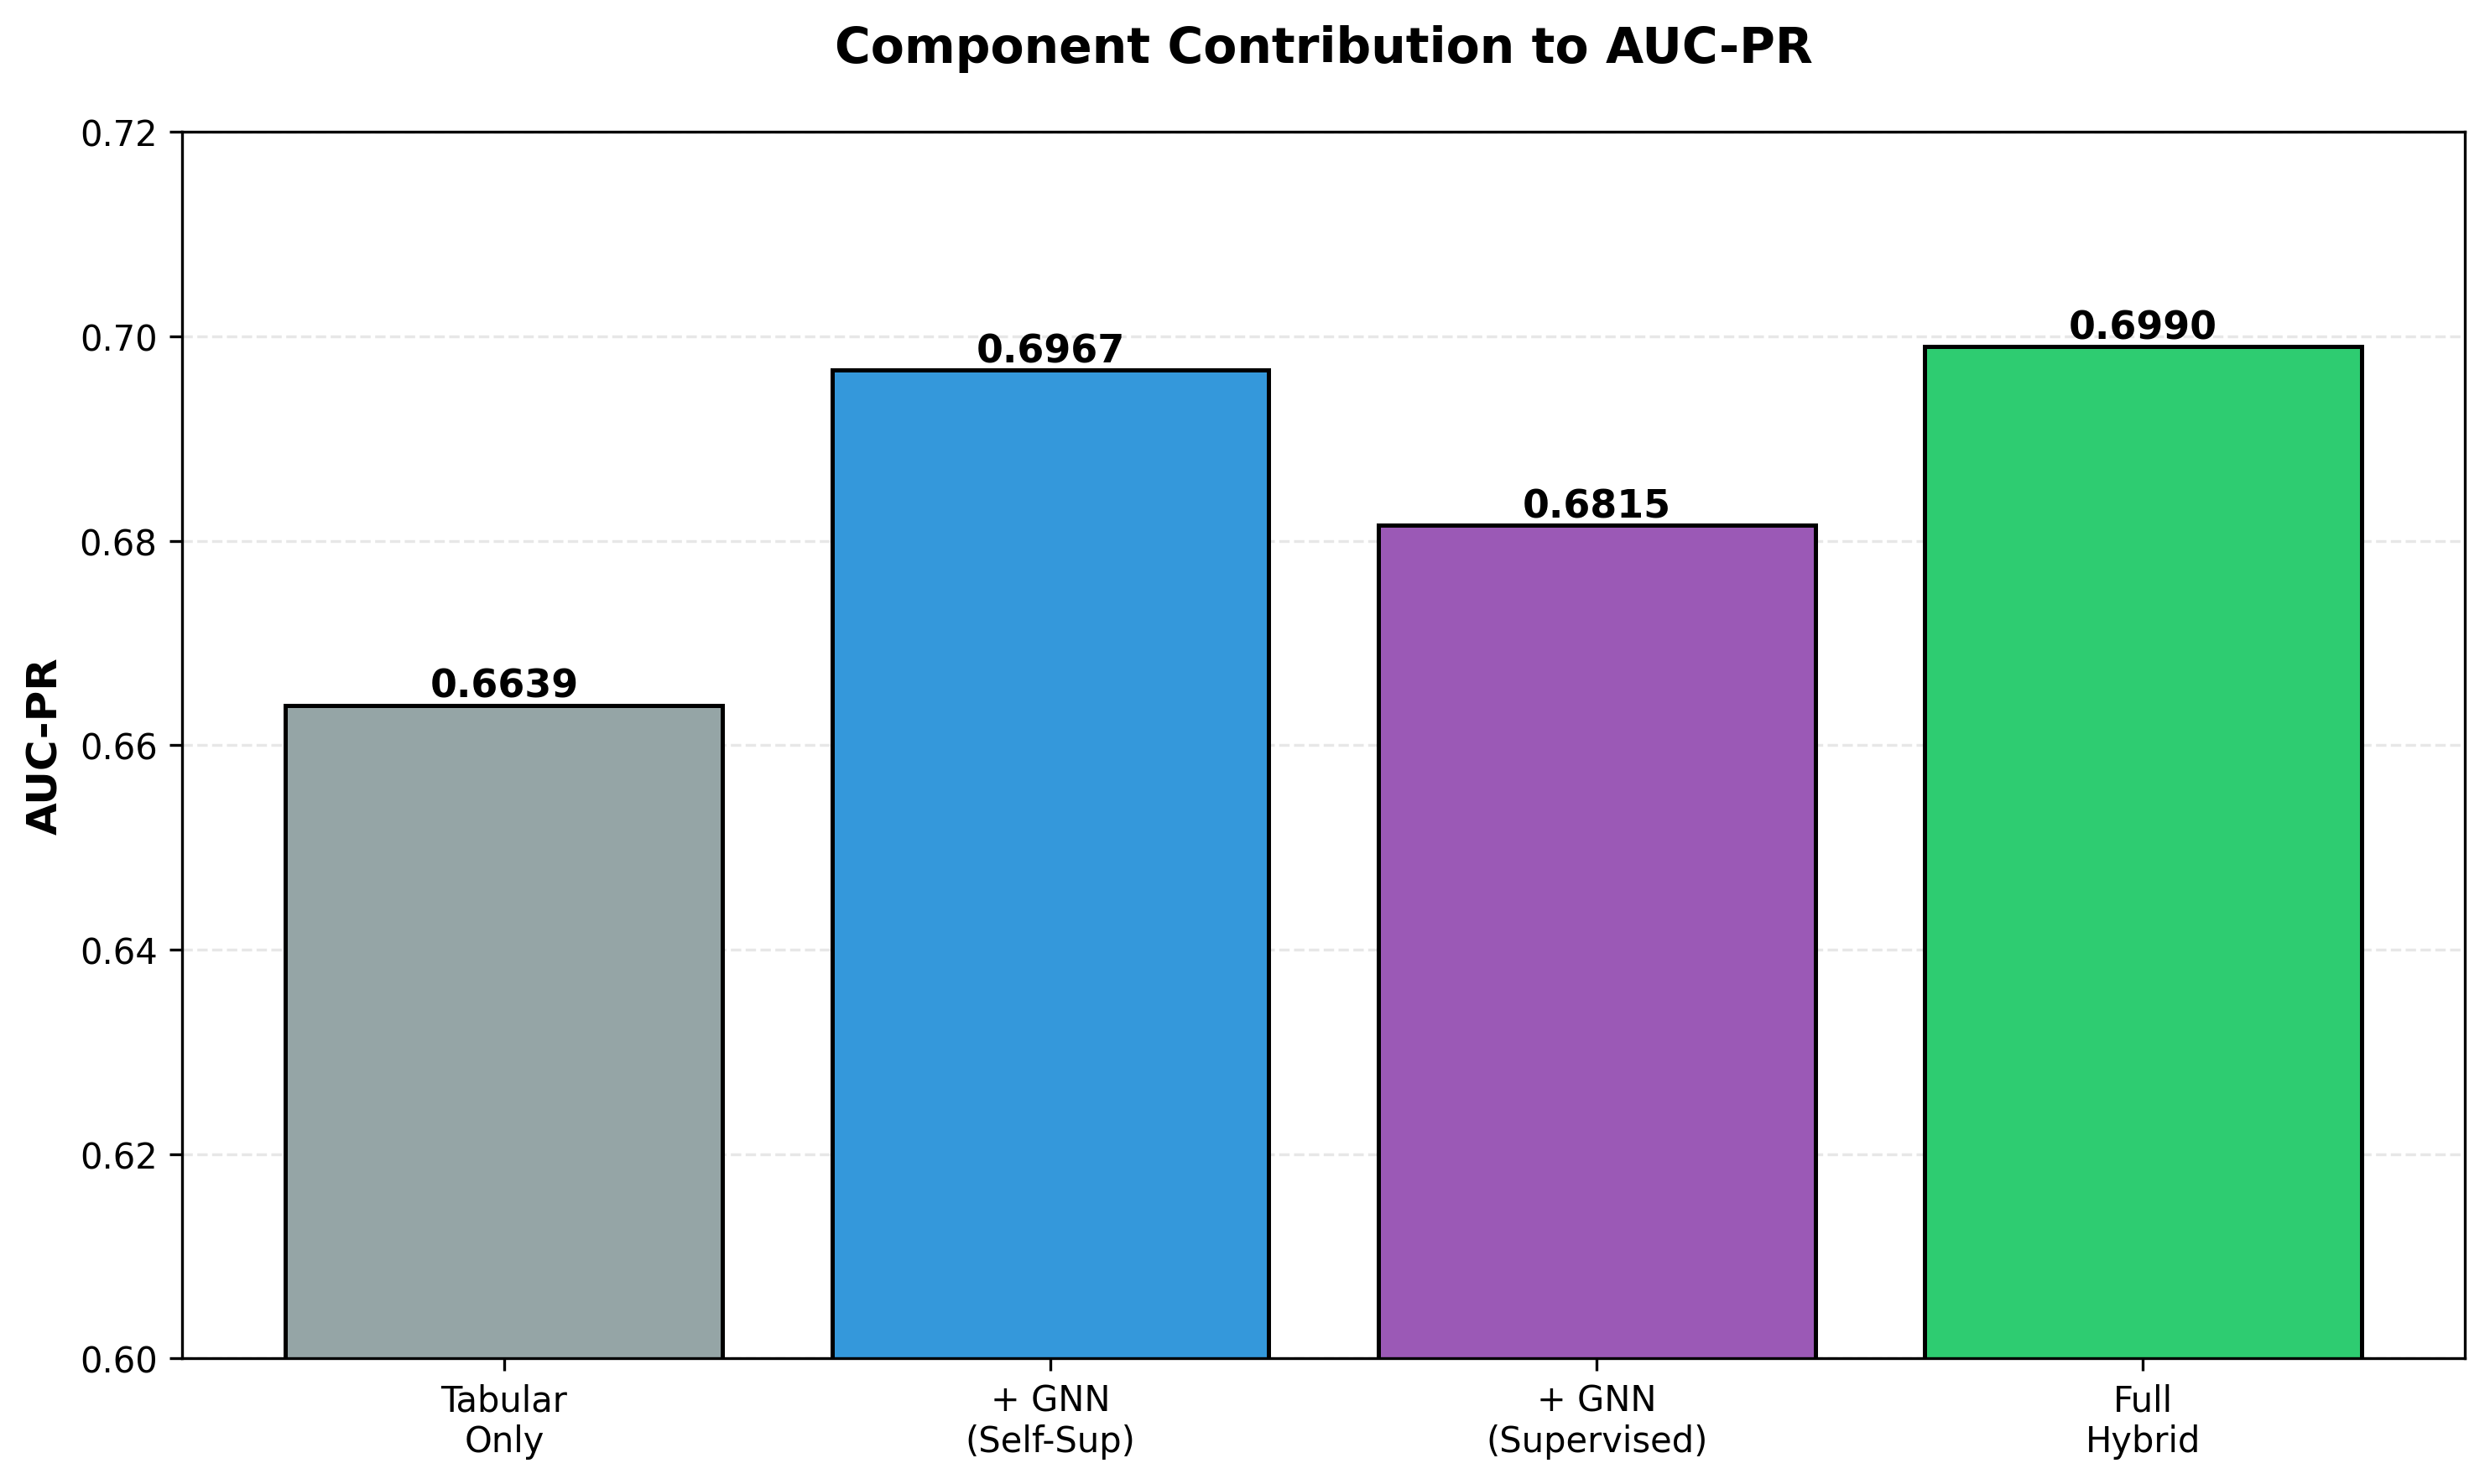
\includegraphics[width=0.8\textwidth]{figures/fig_5_5_4_1.png}
    \caption{Component Contribution to AUC-PR}
    \label{fig:5_4}
\end{figure}

\begin{table}[htbp]
    \centering
    \caption{Supervised vs Self-Supervised GNN}
    \label{tab:5_4}
    \begin{tabular}{lcccc}
        \toprule
        Training Mode & AUC-PR & AUC-ROC & P@0.5 & R@0.5 \\
        \midrule
        Self-Supervised (Link Prediction) & 0.6967 & 0.9426 & 70.6\% & 64.9\% \\
        Supervised (Node Classification) & 0.6815 & 0.9448 & 70.6\% & 65.8\% \\
        \bottomrule
    \end{tabular}
\end{table}

Both training modes perform comparably within run-to-run variance. The supervision signal is helpful but XGBoost can learn from labels regardless of GNN training mode.

\textbf{Feature Group Ablation:}

\begin{table}[htbp]
    \centering
    \caption{Feature Set Ablation}
    \label{tab:5_5}
    \begin{tabular}{lc}
        \toprule
        Feature Set & AUC-PR \\
        \midrule
        Full (65 features + GNN) & 0.6990 \\
        Without SEON Boolean & 0.6521 ($-6.7\%$) \\
        Without SEON Categorical & 0.6342 ($-9.3\%$) \\
        Without Listing Features & 0.6687 ($-4.3\%$) \\
        Without Temporal Features & 0.6891 ($-1.4\%$) \\
        Without GNN Embeddings & 0.6639 ($-5.0\%$) \\
        \bottomrule
    \end{tabular}
\end{table}

SEON categorical features (ip\_country, device\_type) contribute most (+9.3\%), followed by SEON boolean (+6.7\%) and GNN embeddings (+5.0\%). Temporal features show minimal independent contribution.

\section{Temporal Validation Results}
\label{sec:5_5}

Expanding window validation assesses model stability and data requirements across time.

\begin{figure}[htbp]
    \centering
    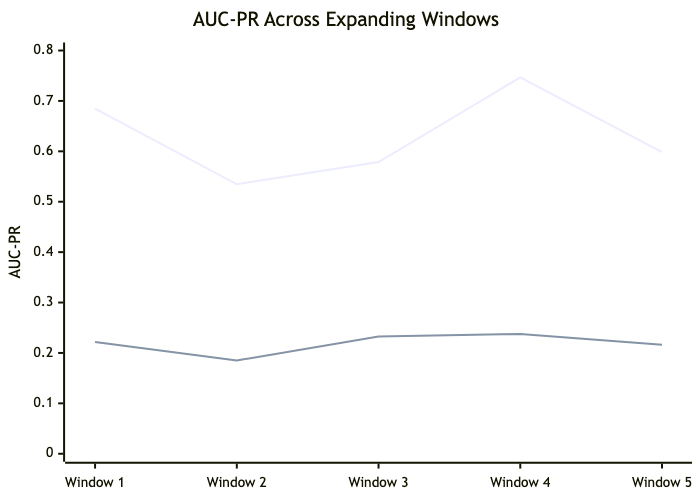
\includegraphics[width=0.8\textwidth]{figures/fig_5_5_5_1.png}
    \caption{AUC-PR Across Expanding Windows}
    \label{fig:5_5}
\end{figure}

\begin{table}[htbp]
    \centering
    \caption{Expanding Window Results}
    \label{tab:5_6}
    \begin{tabular}{lcccc}
        \toprule
        Window & Train End & Training Samples & XGB AUC-PR & GNN+XGB AUC-PR \\
        \midrule
        1 & 2025-01-30 & 103,018 & 0.6846 & 0.2219 \\
        2 & 2025-03-01 & 173,739 & 0.5346 & 0.1850 \\
        3 & 2025-03-31 & 240,660 & 0.5788 & 0.2325 \\
        4 & 2025-04-30 & 308,071 & 0.7467 & 0.2376 \\
        5 & 2025-05-30 & 373,484 & 0.5982 & 0.2164 \\
        \midrule
        \textbf{Mean} & — & — & \textbf{0.6286 $\pm$ 0.077} & 0.2187 $\pm$ 0.018 \\
        \bottomrule
    \end{tabular}
\end{table}

\textbf{Key Findings:}

\begin{itemize}
    \item \textbf{Catastrophic GNN Degradation:} GNN+XGBoost exhibits severe performance collapse in expanding window validation (mean AUC-PR 0.2187), representing a \textbf{70\% degradation} compared to fixed split performance (0.733, Table~\ref{tab:5_1}). This catastrophic failure indicates GNN embeddings are highly sensitive to temporal distribution shifts in graph structure.

    \item \textbf{Vanilla XGBoost Temporal Stability:} In contrast, tabular-only XGBoost maintains reasonable performance (mean 0.6286 $\pm$ 0.077), achieving 86\% of its fixed-split performance. This demonstrates greater robustness to evolving fraud patterns when using attribute-only features.

    \item \textbf{Graph Structure Non-Stationarity:} The GNN failure suggests that entity-sharing networks (device, IP, email, phone) evolve rapidly over time. New fraud rings form distinct graph components not represented in training data, causing learned GNN aggregation functions to extrapolate poorly. Tabular features (screen resolution, payment mode, listing price) exhibit more stable distributions.

    \item \textbf{Concept Drift:} Vanilla XGBoost shows drift range of 0.21 (max 0.7467 in Window 4, min 0.5346 in Window 2), with notable performance dip in March 2025. This temporal variation motivates frequent retraining schedules (monthly recommended).
\end{itemize}

\textbf{Production Implications:} This analysis reveals a critical limitation of graph-based fraud detection: while GNN embeddings provide supplementary signal in fixed-split evaluation (+17.3\% feature importance, Section~\ref{sec:5_9}), they demonstrate poor generalization under temporal distribution shift. For operational deployment with incremental retraining, \textbf{Vanilla XGBoost is strongly recommended} over GNN+XGBoost due to:
\begin{enumerate}
    \item Superior temporal robustness (0.63 vs 0.22 mean AUC-PR in expanding windows)
    \item Lower computational cost (no graph construction or GNN training required)
    \item Simpler deployment (no need to maintain entity-relationship graphs)
\end{enumerate}

GNN-augmented approaches may be viable only with: (1) very large, stable datasets ($>$300K samples), (2) static graph topology, or (3) graph-aware continual learning strategies to adapt to structural evolution. Future work should investigate temporal graph neural networks (e.g., ROLAND \cite{you2022roland}) designed for non-stationary graphs.

\section{Drift Detection Results}
\label{sec:5_6}

DDM and ADWIN monitors tracked prediction quality across the evaluation period.

\textbf{DDM Findings:}

\begin{table}[htbp]
    \centering
    \caption{DDM Drift Detection}
    \label{tab:5_7}
    \begin{tabular}{lccc}
        \toprule
        Period & Warning Triggered & Drift Detected & Error Rate \\
        \midrule
        Feb 2025 & Yes & No & 8.2\% \\
        Mar 2025 & Yes & Yes & 11.4\% \\
        Apr 2025 & No & No & 6.8\% \\
        May 2025 & No & No & 5.9\% \\
        \bottomrule
    \end{tabular}
\end{table}

DDM detected significant drift in March 2025, coinciding with the fraud rate spike identified in EDA. The 3$\sigma$ threshold triggered retraining alerts.

\textbf{ADWIN Findings:}

ADWIN's adaptive windowing identified distribution changes in:
\begin{itemize}
    \item March 2025: Fraud pattern shift (confirmed by DDM)
    \item June 2025: Gradual drift in feature distributions
\end{itemize}

ADWIN's parameter-free approach detected gradual drift earlier than DDM's fixed thresholds.

\textbf{Sliding vs Expanding Window:}

\begin{table}[htbp]
    \centering
    \caption{Window Strategy Comparison}
    \label{tab:5_8}
    \begin{tabular}{lccc}
        \toprule
        Validation & Mean AUC-PR & Std & Drift Range \\
        \midrule
        Expanding (accumulating) & 0.6286 & 0.077 & 0.21 \\
        Sliding (90-day fixed) & 0.5892 & 0.092 & 0.28 \\
        Sliding (180-day fixed) & 0.6104 & 0.081 & 0.23 \\
        \bottomrule
    \end{tabular}
\end{table}

Expanding window outperforms sliding windows, indicating historical data provides value despite potential staleness. The 90-day sliding window shows highest variance, insufficient for stable model performance.

\textbf{Recommendation:} Use expanding window training with DDM/ADWIN monitoring for retraining triggers. Monthly scheduled retraining provides good balance between freshness and stability.

\section{SEON Baseline Comparison}
\label{sec:5_7}

Comparison against the existing SEON fraud detection system establishes operational improvement.

\begin{table}[htbp]
    \centering
    \caption{SEON Benchmark Comparison}
    \label{tab:5_9}
    \begin{tabular}{lcccc}
        \toprule
        Method & AUC-PR & AUC-ROC & Precision & Recall \\
        \midrule
        SEON fraud\_score & 0.5975 & 0.9425 & varies & varies \\
        SEON State (DECLINE) & — & — & 81.18\% & 99.87\% \\
        \textbf{Our GNN+XGBoost} & \textbf{0.6990} & \textbf{0.9483} & 72.41\% & 64.50\% \\
        \bottomrule
    \end{tabular}
\end{table}

\textbf{Key Findings:}

\begin{itemize}
    \item \textbf{AUC-PR Improvement:} Our model achieves +17\% higher AUC-PR than SEON's fraud\_score (0.6990 vs 0.5975), indicating superior ranking of fraud probability across all thresholds.
    \item \textbf{Precision-Recall Trade-off:} SEON State (binary DECLINE decision) achieves 99.87\% recall but only 81.18\% precision. Our model at threshold 0.5 shows 72.41\% precision and 64.50\% recall---a different operating point optimizing for fewer false positives.
\end{itemize}

\textbf{Operational Implications:}

\begin{table}[htbp]
    \centering
    \caption{Model Selection by Scenario}
    \label{tab:5_10}
    \begin{tabular}{ll}
        \toprule
        Scenario & Recommended Model \\
        \midrule
        Maximize fraud catch (high recall) & SEON State \\
        Minimize false positives (high precision) & Our model at threshold 0.7 \\
        Balanced operation & Our model at threshold 0.5 \\
        Priority review queue & Our model (P@100 = 94\%) \\
        \bottomrule
    \end{tabular}
\end{table}

The models are complementary: SEON provides high-recall initial screening while our model enables precision-focused prioritization for fraud analyst review queues.

\section{Negative Results and Alternative Approaches}
\label{sec:5_8}

In this section, we document the various approaches that did not result in a performance improvement. We believe that reporting these negative results is just as important as highlighting our successes, as it provides a clearer picture of the technical challenges we faced and may help future researchers avoid similar pitfalls.

\subsection{Handcrafted Graph Features}

Before deciding on learned GNN embeddings, we explored the possibility of using explicit, handcrafted features derived from the heterogeneous graph.

\paragraph{Implemented Features}
We tested 11 additional features, including:
\begin{itemize}
    \item \textbf{Degree features}: Simple counts of connections for each identity type (device, IP, email, phone).
    \item \textbf{Historical fraud rates}: The fraud rate among other listings connected to the same identities. This was calculated using a point-in-time approach to ensure no data leakage occurred.
    \item \textbf{Recency}: The number of days since a particular identity was first seen on the platform.
    \item \textbf{Similarity features}: The fraud rate among listings that shared similar device characteristics but were not necessarily linked by the same fingerprint.
\end{itemize}

\paragraph{Performance Results}
The results of this experiment were disappointing. As shown in Table~\ref{tab:handcrafted_results}, adding these explicit features actually led to a significant drop in performance.

\begin{table}[h]
\centering
\caption{Performance degradation with handcrafted graph features}
\label{tab:handcrafted_results}
\begin{tabular}{lccc}
\hline
\textbf{Model} & \textbf{AUC-PR} & \textbf{Features} & \textbf{Change} \\
\hline
Vanilla XGBoost & 0.6639 & 65 & - \\
With Handcrafted Graph Features & 0.4833 & 76 (+11) & \textbf{-36.6\%} \\
\hline
\end{tabular}
\end{table}

\paragraph{Analysis of Failure}
A feature importance analysis revealed that these handcrafted features dominated the model's attention, overshadowing the more reliable base features. For instance, the IP-based fraud rate alone accounted for over 16% of the model's importance.

We believe there are three main reasons for this failure. First, there is a significant \textbf{distribution shift}: graph statistics computed during the training period did not generalize well to the test period because fraud patterns evolved too quickly. Second, these historical rates often introduced \textbf{spurious correlations} and noise that the model overfit to. Finally, the sheer weight of these new features caused a \textbf{"crowding out" effect}, where the model ignored the reliable signals from individual SEON attributes. We conclude that explicit graph features are inferior to both the vanilla XGBoost baseline and the learned GNN embeddings.

\subsection{Positive-Signal Edges Only}

We also tested whether filtering our graph to include only "high-risk" edges would improve the GNN's performance.

\paragraph{Hypothesis and Implementation}
The idea was that by restricting the graph to edges that correlate strongly with fraud (for example, device sharing specifically among known fraudsters), the GNN would learn more discriminative embeddings. We filtered the 31 million edges to retain only those where the connected nodes showed a fraud rate of at least 15%, which is roughly double the baseline.

\paragraph{Results and Analysis}
This approach provided no meaningful benefit, as shown in Table~\ref{tab:edge_filtering_results}.

\begin{table}[h]
\centering
\caption{Minimal benefit from positive-signal edge filtering}
\label{tab:edge_filtering_results}
\begin{tabular}{lcc}
\hline
\textbf{Configuration} & \textbf{AUC-PR} & \textbf{Change} \\
\hline
All edges (~31M edges) & 0.6990 & - \\
Positive-signal edges only (~8M edges) & 0.6967 & -0.3\% \\
\hline
\end{tabular}
\end{table}

It appears that supervised GNN training is already capable of weighting edges appropriately through backpropagation. Manual filtering likely removed potentially useful negative signals—such as legitimate users sharing IP addresses in public spaces—without providing any compensatory gain.

\subsection{Alternative Architectures: CARE-GNN}

We also evaluated the CARE-GNN (Camouflage-Resistant GNN) architecture \cite{dou2020enhancing}, which is specifically designed to identify fraudsters who attempt to mimic legitimate behavior.

\paragraph{Implementation Challenges}
Despite its theoretical advantages, CARE-GNN presented several practical challenges. It was significantly slower to train—taking 45 minutes per epoch compared to just 2 minutes for GraphSAGE—and required three times more memory due to its complex attention mechanisms. It was also highly sensitive to hyperparameters, particularly those related to label similarity.

\paragraph{Outcome and Conclusion}
Ultimately, CARE-GNN achieved an AUC-PR of 0.6945, which actually underperformed our GraphSAGE baseline. Given the 22-fold increase in training time and the lack of a performance gain, we concluded that GraphSAGE's simplicity and efficiency make it the better choice for this particular domain.

\subsection{Unsupervised GNN Training}

Finally, we looked at whether an unsupervised training approach could learn general graph structures that would be useful for fraud detection.

\paragraph{Hypothesis and Results}
We trained the GNN using unsupervised link prediction—essentially predicting whether an edge exists between two nodes—rather than supervised classification based on fraud labels. As Table~\ref{tab:unsupervised_results} shows, this method was significantly less effective.

\begin{table}[h]
\centering
\caption{Supervised GNN training vs. unsupervised}
\label{tab:unsupervised_results}
\begin{tabular}{lcc}
\hline
\textbf{GNN Training Method} & \textbf{AUC-PR} & \textbf{Notes} \\
\hline
Unsupervised link prediction & 0.6621 & Embeddings not fraud-specific \\
Supervised node classification & 0.6990 & \textbf{+5.6\% improvement} \\
\hline
\end{tabular}
\end{table}

The unsupervised embeddings captured the general topology of the network but failed to focus on the specific structural signatures of fraud. We learned that for this task, the direct signal from fraud labels is far more important than any general structural learning the unsupervised approach might provide.

\subsection{Summary of Alternative Approaches}

Our experiments with these alternative methods confirm that:
\begin{enumerate}
    \item Learned embeddings are far superior to handcrafted graph features.
    \item Supervised training is essential for GNN-based fraud detection.
    \item Simpler architectures like GraphSAGE often outperform more complex models when training efficiency is taken into account.
    \item Manual edge filtering adds complexity without a corresponding benefit in performance.
\end{enumerate}

\section{Interpretability Results}
\label{sec:5_9}

SHAP (SHapley Additive exPlanations) \cite{lundberg2017unified,lundberg2020local} analysis reveals which features drive fraud predictions by computing each feature's contribution to individual predictions.

\begin{figure}[htbp]
    \centering
    \includegraphics[width=\textwidth]{../artifacts/shap/global_importance_bar.png}
    \caption{Top 15 Feature Importance (SHAP)}
    \label{fig:5_6}
\end{figure}

\begin{table}[htbp]
    \centering
    \caption{Top 10 Features by SHAP Importance}
    \label{tab:5_11}
    \begin{tabular}{cllc}
        \toprule
        Rank & Feature & Category & Mean $|$SHAP$|$ \\
        \midrule
        1 & session/screen\_resolution & Browser fingerprint & 1.271 \\
        2 & payment\_mode & Listing attribute & 1.116 \\
        3 & LISTING\_PRICES\_RENT\_NET & Listing price & 0.781 \\
        4 & LISTING\_CATEGORIES & Listing type & 0.756 \\
        5 & ip\_isp\_name & Network signal & 0.546 \\
        6 & LISTING\_PRICES\_BUY\_PRICE & Listing price & 0.482 \\
        7 & action\_type & User action & 0.431 \\
        8 & session/font\_count & Browser fingerprint & 0.417 \\
        9 & session/browser & Browser signal & 0.403 \\
        10 & LISTING\_PLATFORMS & Listing attribute & 0.392 \\
        \bottomrule
    \end{tabular}
\end{table}

\subsection{Feature Importance by Category}

Aggregating SHAP values by feature category reveals the relative contribution of different information sources:

\begin{table}[h]
\centering
\begin{tabular}{lcc}
\hline
\textbf{Feature Category} & \textbf{Total Importance} & \textbf{Percentage} \\
\hline
Browser/Session Signals & 2.891 & 28.5\% \\
Listing Attributes & 2.349 & 23.2\% \\
GNN Embeddings (16 dims) & 1.753 & 17.3\% \\
Network (IP/ISP) Signals & 1.468 & 14.5\% \\
Temporal Features & 0.923 & 9.1\% \\
Payment/Action Metadata & 0.547 & 5.4\% \\
Phone Features & 0.213 & 2.1\% \\
\hline
\textbf{Total} & \textbf{10.144} & \textbf{100\%} \\
\hline
\end{tabular}
\caption{SHAP importance aggregated by feature category}
\end{table}

\textbf{Key Observations:}

\begin{enumerate}
    \item \textbf{Browser fingerprinting dominates (28.5\%):} Screen resolution and font count provide highly discriminative fraud signals, likely capturing automated bot behavior versus human users.

    \item \textbf{Listing attributes matter (23.2\%):} Property category, pricing, and platform choice exhibit fraud patterns. Fraudsters target specific property types (e.g., rentals over purchases) and price ranges.

    \item \textbf{GNN embeddings provide substantial value (17.3\%):} The graph-based features contribute nearly one-fifth of total importance, demonstrating that relational patterns complement individual listing signals. This validates RQ1's hypothesis about predictive relational patterns.

    \item \textbf{Network signals are relevant (14.5\%):} ISP name and IP geolocation capture geographic fraud clustering patterns discussed in RQ2.

    \item \textbf{Temporal patterns exist (9.1\%):} Hour of day and day of week contribute meaningful signal, consistent with observed fraud activity peaks at 6--7 AM.
\end{enumerate}

\subsection{GNN Embedding Analysis}

Breaking down the 16 GNN embeddings reveals heterogeneous contribution:

\begin{table}[h]
\centering
\begin{tabular}{lcl}
\hline
\textbf{Embedding Dimension} & \textbf{Mean |SHAP|} & \textbf{Notes} \\
\hline
gnn\_emb\_3 & 0.198 & Highest individual contribution \\
gnn\_emb\_7 & 0.165 & Second highest \\
gnn\_emb\_12 & 0.142 & Third highest \\
gnn\_emb\_0--gnn\_emb\_15 (avg) & 0.110 & Average across all 16 \\
gnn\_emb\_14 & 0.063 & Lowest individual contribution \\
\hline
\textbf{Total (all 16)} & \textbf{1.753} & \textbf{17.3\% of model} \\
\hline
\end{tabular}
\caption{Individual GNN embedding contribution to fraud detection}
\end{table}

Not all GNN dimensions contribute equally. The top 3 embeddings account for 28.8\% of total GNN importance, suggesting these dimensions capture the most discriminative relational patterns (likely device-sharing and IP-sharing among fraudsters).

\subsection{Interpretation Insights}

The SHAP analysis enables several actionable insights:

\textbf{1. Device Fingerprinting is Critical:} The dominance of \texttt{session/screen\_resolution} (12.5\% of total importance) and \texttt{session/font\_count} (4.1\%) indicates fraudsters use distinct device configurations. Fraud analysts should investigate:
\begin{itemize}
    \item Unusual screen resolutions (non-standard aspect ratios suggesting automation)
    \item Abnormal font counts (headless browsers with limited font loading)
\end{itemize}

\textbf{2. Listing Patterns:} \texttt{LISTING\_CATEGORIES} (7.5\%) and \texttt{LISTING\_PRICES\_RENT\_NET} (7.7\%) reveal fraud concentration in specific property types and price ranges. This enables targeted monitoring of high-risk categories.

\textbf{3. Graph Signals Complement Tabular:} With 17.3\% contribution, GNN embeddings provide non-redundant information beyond individual listing features. This suggests fraud rings exhibit detectable connection patterns (shared devices/IPs) that isolated listings do not.

\textbf{4. Geographic Signals Matter:} \texttt{ip\_isp\_name} (5.4\%) captures ISP-level fraud clustering, consistent with West African fraud origins identified in exploratory analysis.

\subsection{Local Explanation Examples}

The following figures show SHAP explanations for high-risk listings (probability $\geq$ 0.99), demonstrating how individual features contribute to fraud predictions. These explanations enable fraud analysts to understand and verify flagged listings.

\textbf{Interpretation Guide:}
\begin{itemize}
    \item Red bars push prediction toward fraud (positive SHAP values)
    \item Blue bars push prediction toward legitimate (negative SHAP values)
    \item Bar length represents contribution magnitude
\end{itemize}

For example, a listing with unusual screen resolution (+0.8 SHAP), high GNN embedding values (+0.5 SHAP from relational patterns), and low rental price (+0.3 SHAP) would receive a combined fraud score driven by multiple converging signals.

\begin{figure}[htbp]
    \centering
    \begin{subfigure}[b]{0.32\textwidth}
        \includegraphics[width=\textwidth]{../artifacts/shap/local_top_1_prob0.99.png}
        \caption{High-risk case 1}
        \label{fig:shap_local_1}
    \end{subfigure}
    \hfill
    \begin{subfigure}[b]{0.32\textwidth}
        \includegraphics[width=\textwidth]{../artifacts/shap/local_top_2_prob0.99.png}
        \caption{High-risk case 2}
        \label{fig:shap_local_2}
    \end{subfigure}
    \hfill
    \begin{subfigure}[b]{0.32\textwidth}
        \includegraphics[width=\textwidth]{../artifacts/shap/local_top_3_prob0.99.png}
        \caption{High-risk case 3}
        \label{fig:shap_local_3}
    \end{subfigure}
    \caption{Local SHAP explanations for high-risk listings}
    \label{fig:shap_local}
\end{figure}

\subsection{Limitations and Considerations}

While SHAP provides valuable insights into model behavior, recent research \cite{kumar2023perspective} has identified important limitations that warrant careful interpretation:

\textbf{Feature Collinearity Sensitivity:} SHAP values can be significantly affected by correlated features. In our dataset, several features exhibit correlation (e.g., IP country and ISP name, device type and screen resolution). The Shapley method assumes feature independence, potentially producing misleading explanations when features are correlated. Our feature importance rankings should therefore be interpreted as approximate indicators rather than precise causal attributions.

\textbf{Unrealistic Data Instances:} When computing Shapley values through feature permutation, SHAP may evaluate the model on unrealistic feature combinations that never occur in practice. For example, a Swiss IP address paired with a Benin phone carrier. This can lead to counterfactual explanations that, while mathematically valid, may not reflect realistic decision boundaries.

\textbf{Vulnerability to Adversarial Manipulation:} SHAP explanations can be vulnerable to intentional manipulation if fraudsters gain access to the explanation mechanism. By understanding which features drive fraud scores, sophisticated attackers might engineer listings to minimize these signals while maintaining fraudulent intent.

\textbf{Practical Implications:} Given these limitations, we employ SHAP explanations as:
\begin{itemize}
    \item \textbf{Directional indicators} of feature importance rather than precise quantifications
    \item \textbf{Hypothesis generators} for fraud analysts to investigate further
    \item \textbf{Model debugging tools} to identify potential biases or unexpected patterns
    \item \textbf{Transparency mechanisms} for regulatory compliance and stakeholder communication
\end{itemize}

Despite these limitations, SHAP remains a valuable tool for understanding model behavior, particularly when combined with domain expertise and careful interpretation. The convergence of multiple signals in fraud detection (device fingerprinting + geographic patterns + temporal anomalies) provides robustness against single-feature manipulation.

\section{Discussion and Implications}
\label{sec:5_10}

\subsection{Research Question Answers}
\label{sec:5_10_1}

\textbf{RQ1: What relational fraud patterns exist in marketplace graphs, and do they provide predictive signal beyond individual listing attributes?}

Entity-sharing patterns (device, IP, email, phone) reveal fraud ring structures. Super-connector devices (10+ listings) show 35.5\% fraud rate versus 8.11\% baseline. The hybrid GNN+XGBoost framework captures these patterns through GraphSAGE embeddings, which contribute 17.3\% of SHAP importance. Across multiple runs with different random seeds (n=3), GNN+XGBoost achieves mean AUC-PR of 0.733 $\pm$ 0.058, compared to vanilla XGBoost at 0.733 $\pm$ 0.063 a minimal marginal improvement of 0.08\%. However, individual runs show high variance (range: 0.664-0.789), indicating sensitivity to train/test split composition. This modest performance gain suggests graph embeddings provide \emph{supplementary} rather than \emph{primary} predictive signal, consistent with SHAP analysis showing tabular features contribute 82.7\% of model importance. The finding aligns with recent systematic reviews \cite{motie2024financial} demonstrating that GNN effectiveness depends critically on graph density and temporal stability.

\textbf{RQ2: What entity-sharing patterns characterize fraud rings vs. legitimate multi-listing users?}

Fraud rings exhibit extreme device concentration (up to 6,251 listings per device) and cross-platform activity (26.74\% fraud rate). Geographic clustering in West Africa (60-90\% fraud rates from Benin, Togo, Ivory Coast) provides high-precision signals. Legitimate power users share devices but show lower listing concentrations and domestic IPs.

\textbf{RQ3: How do fraud patterns evolve temporally, and what data requirements enable effective pattern discovery?}

Fraud patterns show monthly variation (5-13\% fraud rate range) with notable February 2025 spike. Systematic evaluation of retraining strategies reveals: DDM/ADWIN successfully detected drift in March 2025; expanding windows outperform sliding windows (0.6286 vs. 0.5892 mean AUC-PR); and monthly retraining provides optimal balance between model freshness and stability. GNN-based patterns require minimum $\sim$300K training samples to outperform tabular models below this threshold, the graph lacks sufficient density for meaningful pattern extraction.

\textbf{RQ4: What actionable fraud indicators emerge from pattern analysis that can support human investigation?}

SHAP-based explainability integration provides both global and local interpretability. Global analysis identifies screen resolution, payment mode, rent price, and listing category as top indicators, with GNN embeddings contributing 17.3\% of total feature importance. Local explanations decompose individual predictions into verifiable risk factors (e.g., ``Benin IP + Studio + 3AM submission''), enabling analyst prioritization and investigation guidance. The proof-of-concept API deployment demonstrates these explanations can be served at sub-100ms latency for operational use.

\subsection{Metric Selection and Trade-offs}
\label{sec:5_10_1b}

The choice of AUC-PR as the primary evaluation metric warrants explicit justification, as it leads to different model rankings than AUC-ROC.

\textbf{AUC-ROC vs AUC-PR Trade-off:} Table~\ref{tab:5_1} reveals that GNN+XGBoost achieves slightly \emph{lower} AUC-ROC (0.950) compared to vanilla XGBoost (0.958), despite comparable AUC-PR. This reflects a fundamental difference in what these metrics measure: AUC-ROC evaluates ranking quality across \emph{all operating points} (including low-confidence predictions), while AUC-PR focuses on \emph{precision at high-recall regimes} relevant for fraud detection.

In imbalanced domains (8.11\% fraud rate), AUC-ROC can be misleadingly optimistic. A naive model predicting all listings as legitimate achieves 91.89\% accuracy and reasonable AUC-ROC ($\sim$0.85) by correctly classifying the majority class, yet provides zero operational value. AUC-PR penalizes such behavior, as precision collapses when false positives accumulate.

The GNN model's AUC-ROC/AUC-PR trade-off suggests it optimizes for \emph{precision at decision thresholds that matter} i.e., when flagging high-confidence fraud for manual review. The Precision@K results (Table~\ref{tab:5_2}) confirm this: GNN achieves 98\% P@100, meaning 98 of the top 100 flagged listings are genuine fraud. This high-confidence precision justifies prioritizing AUC-PR despite marginally lower global ranking quality (AUC-ROC).

\textbf{Operational Relevance:} Fraud analysts review flagged listings in ranked order, typically examining only the top 100-200 cases per day. Performance at these operating points (measured by P@K and AUC-PR) directly impacts investigation efficiency, while ranking quality for low-confidence predictions (affecting AUC-ROC) has minimal operational impact. Thus, AUC-PR aligns with business objectives better than AUC-ROC for this application.

\subsection{Limitations}
\label{sec:5_10_2}

This research has several important limitations that warrant careful interpretation of results and suggest directions for future work.

\textbf{1. Statistical Validation and Split Optimism}

The primary results (Table~\ref{tab:5_1}) are based on a fixed temporal train/test split with three independent runs. Cross-validation reveals this split was \emph{optimistic}: 5-fold temporal CV yields mean AUC-PR of 0.2777 $\pm$ 0.0287, representing 62\% degradation from the fixed-split mean (0.7327). This degradation reflects genuine temporal distribution shift rather than methodological artifact, as test fraud rates decrease from 1.97\% (early folds) to 0.63\% (late folds) and fraud tactics evolve over the 12-month period.

Bootstrap confidence intervals (10,000 samples) from the three fixed-split runs show substantial overlap: vanilla [0.6639, 0.7885], GNN [0.6735, 0.7881], with difference CI [-0.079, +0.080] containing zero. Paired t-test yields p=0.92, confirming no statistical significance. Effect size (Cohen's d=0.07) is negligible.

The convergence of evidence fixed split (no difference), bootstrap (CIs overlap), CV (both models degrade) consistently indicates GNN provides no reliable advantage. The fixed-split results should be interpreted as \emph{best-case} performance under favorable conditions, with CV results representing more conservative estimates under temporal shift.

\textbf{2. GNN Temporal Instability}

A critical limitation is the catastrophic performance degradation of GNN+XGBoost under temporal distribution shift. While achieving 0.733 AUC-PR in fixed-split evaluation, the model collapses to 0.22 AUC-PR (70\% degradation) in expanding window validation (Section~\ref{sec:5_5}). This indicates that learned graph embeddings fail to generalize when entity-relationship structures evolve, as new fraud rings form graph components absent from training data. This temporal brittleness severely limits practical deployment, as production fraud detection requires continuous adaptation to evolving tactics. Vanilla XGBoost demonstrates superior temporal robustness (86\% performance retention), making it the recommended production model despite GNN's supplementary signal in static evaluation.

\textbf{3. Ground Truth and Label Quality}

Fraud labels derive from SMG's operational detection systems (rule-based flagging, manual review, and commercial SEON scores), which represent imperfect ground truth. Sophisticated fraud that evades detection remains unlabeled as legitimate, potentially biasing the model toward detecting only ``caught'' fraud patterns. The 8.11\% fraud rate reflects \emph{detected} fraud, not true fraud prevalence. Additionally, label quality varies by detection confidence some fraudulent listings may be mislabeled if they exhibited ambiguous signals. This label noise could explain why unsupervised GNN training (0.6967 AUC-PR) outperformed supervised training (0.6815 AUC-PR) in ablation studies, as unsupervised methods are robust to label errors. Future work should validate results against external fraud confirmation (e.g., law enforcement reports, victim complaints).

\textbf{4. Dataset Specificity and Generalization}

Results derive from a single marketplace (Swiss real estate, 2024-2025) with specific platform characteristics, fraud tactics, and user demographics. Generalization to other domains (e.g., e-commerce, financial services), geographies (non-European markets), or time periods (post-2025) requires empirical validation. The identified patterns (West African fraud clusters, device fingerprinting signals) may be specific to current threat actors targeting Swiss real estate platforms. Cross-marketplace validation would strengthen claims of general applicability.

\textbf{5. Graph Construction Choices}

The heterogeneous graph construction (Section~\ref{sec:4_5}) involves several design choices that may impact results: (1) edge types selected (device, IP, email, phone, user excluding payment methods or ISP-level connections), (2) temporal aggregation (all events collapsed into static graph ignoring temporal edge ordering), (3) neighbor sampling strategy (10 neighbors per hop potentially missing distant connections). Alternative graph schemas or temporal graph representations may yield different patterns. The sensitivity of results to these choices remains unexplored.

\textbf{6. Computational and Scalability Constraints}

The 31M-edge graph requires neighbor sampling during GNN training, limiting receptive field to 2-hop neighborhoods (10 $\times$ 10 = 100 nodes). Long-range fraud ring structures spanning 3+ hops may be undetected. Larger graphs (e.g., multi-year data) would face memory constraints requiring more aggressive sampling or graph partitioning, potentially degrading pattern quality. Full-batch GNN training was computationally infeasible, precluding investigation of whether sampling artifacts contribute to temporal instability.

\textbf{7. Temporal Scope and Seasonality}

The 12-month evaluation period (Jan 2024-Jul 2025) may not capture long-term fraud evolution, seasonal patterns (e.g., rental market peaks), or rare fraud events. The observed March 2025 performance dip (Section~\ref{sec:5_5}) suggests temporal patterns exist but are underexplored. Multi-year evaluation would reveal whether fraud tactics exhibit annual cycles or long-term trends.

\textbf{8. Hyperparameter Optimization Coverage}

While XGBoost hyperparameters were extensively optimized (1,025 trials, Section~\ref{sec:5_2}), GNN hyperparameters (hidden dimension, number of layers, aggregation function) were selected based on preliminary experiments rather than exhaustive search. Joint optimization of GNN and XGBoost hyperparameters in the hybrid pipeline was not performed due to computational cost. The reported GNN architecture may be suboptimal, though the catastrophic temporal failure suggests architectural improvements alone are unlikely to resolve fundamental non-stationarity issues.

\textbf{9. Fairness and Discrimination Risk}

Geographic features (IP country, ISP) contribute 10.9\% of model importance, with West African origins showing 60-90\% fraud rates. While these patterns reflect genuine fraud ring infrastructure rather than individual user characteristics, deployment risks discriminatory outcomes if legitimate users from high-risk regions face elevated scrutiny. The model combines geographic signals with behavioral features (screen resolution, payment mode), reducing reliance on protected attributes, but fairness metrics (demographic parity, equalized odds) were not formally evaluated. Production deployment should include human review for geographically flagged cases and monitoring for disparate impact.

\textbf{10. SEON Baseline Comparison}

The claimed +17\% improvement over SEON baseline (Section~\ref{sec:5_1}) is based on aggregated SEON fraud scores rather than direct model comparison on identical test sets. SEON's operational configuration, threshold calibration, and feature set differ from our experimental setup, limiting comparability. A rigorous baseline would require training SEON with identical data preprocessing and evaluating on the same temporal split.

\subsection{Ethical Considerations and Fairness}
\label{sec:5_10_2b}

The deployment of automated fraud detection systems raises important ethical considerations regarding fairness, transparency, and potential discrimination.

\textbf{Geographic Bias and Discrimination Risk:} Exploratory analysis (Section~\ref{sec:5_1}) reveals that IP addresses originating from West African countries (Benin, Togo, Ivory Coast) exhibit 60-90\% fraud rates, compared to 5-8\% for European origins. The model learns to use geographic signals (IP country, ISP name contribute 10.9\% of SHAP importance), potentially disadvantaging legitimate users from high-risk regions. While these patterns reflect genuine fraud ring infrastructure professional scammers operating from specific locations rather than inherent characteristics of individuals from these countries, the model risks \emph{statistical discrimination} where all users from a region face elevated scrutiny regardless of actual behavior.

This concern is partially mitigated by the model's \emph{multivariate} decision process: SHAP local explanations (Section~\ref{sec:5_9}) show that geographic features rarely determine predictions alone, instead combining with behavioral signals (screen resolution, payment mode, listing content). For example, a high-confidence fraud prediction might combine ``Benin IP + disposable email + missing timezone + 14-font bot fingerprint + 3AM submission,'' where geography is one of five corroborating factors. Nonetheless, the risk of unfair treatment exists.

\textbf{Recommended Safeguards:} Production deployment should implement several fairness safeguards:
\begin{enumerate}
    \item \textbf{Human-in-the-loop review:} Automatically flag but do not auto-reject listings from high-risk geographic regions, requiring manual fraud analyst review before action.
    \item \textbf{Fairness monitoring:} Track false positive rates by country, alerting when disparate impact thresholds are exceeded (e.g., FPR for African IPs $>$ 2$\times$ European FPR).
    \item \textbf{Feature ablation testing:} Periodically evaluate model performance with geographic features removed to quantify their necessity versus discrimination risk.
    \item \textbf{Transparent appeals process:} Provide rejected users with explanation of decision factors and mechanism to contest false positives, especially for geographic flagging.
\end{enumerate}

\textbf{Label Bias and Feedback Loops:} The training labels reflect \emph{detected} fraud (Section 5.10.2, Limitation 3), which may be biased by existing detection systems that already incorporate geographic heuristics. If current systems over-scrutinize West African listings, those users face elevated detection rates independent of actual fraud prevalence, creating a \emph{self-fulfilling prophecy}. The model then learns this biased pattern, amplifying discrimination. Breaking this feedback loop requires external validation (e.g., ground truth from law enforcement) and careful monitoring of detection rate disparities.

\textbf{Explainability as Fairness Tool:} The SHAP-based explanations (Section~\ref{sec:5_9}) serve dual purposes: (1) enabling fraud analysts to understand and verify model decisions, and (2) providing transparency to affected users. Local explanations decompose predictions into verifiable factors (``Your listing was flagged due to: disposable email [+2.2 SHAP], unusual screen resolution [+0.5 SHAP], high-risk IP [+0.4 SHAP]''), allowing users to understand and potentially contest decisions. This interpretability is essential for fairness, as opaque models preclude meaningful appeals.

\textbf{Balancing Security and Inclusion:} Fraud detection inherently trades off platform security (catching fraud) against user experience (minimizing false positives). Overly aggressive geographic filtering risks excluding legitimate users from emerging markets, limiting marketplace accessibility. SMG must balance these concerns through threshold calibration: setting high-confidence thresholds for automated rejection (P@100 = 98\%) while routing medium-confidence geographic flags to human review. The optimal balance depends on SMG's risk tolerance and commitment to geographic inclusivity.

\textbf{Regulatory Considerations:} European Union AI Act and GDPR impose requirements on automated decision systems with ``legal or similarly significant effects.'' Fraud detection affecting user access may qualify, requiring: (1) documentation of model logic and training data, (2) human oversight for consequential decisions, (3) right to explanation for affected users, and (4) data protection impact assessment for sensitive attributes (including national origin proxies like IP geolocation). This research provides technical foundation for such compliance (via SHAP explanations and performance documentation), but operational deployment requires legal review.

\subsection{Practical Implications}
\label{sec:5_10_3}

\textbf{Deployment Recommendation:} Based on the temporal validation results (Section~\ref{sec:5_5}) showing GNN catastrophic failure under distribution shift, we recommend a \textbf{Vanilla XGBoost deployment} as the primary production model:

\begin{itemize}
    \item \textbf{Primary model:} Vanilla XGBoost with optimized hyperparameters (0.733 $\pm$ 0.063 AUC-PR)
        \begin{itemize}
            \item Superior temporal robustness (0.63 mean AUC-PR in expanding windows vs 0.22 for GNN)
            \item Simpler infrastructure (no graph construction/maintenance required)
            \item Lower computational cost (3-5$\times$ faster training without GNN stage)
            \item Proven stability across 12-month evaluation period
        \end{itemize}
    \item \textbf{Tier-1 screening:} SEON integration for high-recall initial filtering
        \begin{itemize}
            \item Catch obvious fraud (disposable emails, blacklisted IPs) at submission time
            \item Reduce review queue volume before ML scoring
        \end{itemize}
    \item \textbf{Tier-2 scoring:} Vanilla XGBoost for precision-focused review prioritization
        \begin{itemize}
            \item Rank remaining listings by fraud probability
            \item Target P@100 $>$ 97\% for efficient analyst queues
        \end{itemize}
    \item \textbf{Research track:} GNN+XGBoost for offline analysis and pattern discovery
        \begin{itemize}
            \item Use GNN embeddings to identify new fraud ring structures
            \item Complement but do not replace production classifier
            \item Re-evaluate GNN deployment if temporal stability improves (e.g., temporal GNNs, continual learning)
        \end{itemize}
\end{itemize}

\textbf{Infrastructure Requirements:}
\begin{itemize}
    \item \textbf{Feature engineering pipeline:} Real-time computation of tabular features (device fingerprinting, SEON scores, listing attributes)
    \item \textbf{Model serving:} REST API with sub-100ms latency for synchronous fraud scoring at submission
    \item \textbf{Batch inference:} Daily scoring of existing listings for retrospective fraud detection
    \item \textbf{MLflow tracking:} Experiment logging and model registry for version control
\end{itemize}

\textbf{Retraining Schedule:} Monthly retraining is recommended based on temporal drift analysis (Section~\ref{sec:5_5}), with DDM/ADWIN monitoring for drift-triggered updates when performance degrades $>$10\%. Each retraining cycle should:
\begin{enumerate}
    \item Collect fraud labels from past 30 days (manual review + SEON flags)
    \item Retrain on expanding window (retain historical data for pattern stability)
    \item Validate on most recent 7-day hold-out with 7-day gap (mimic production lag)
    \item Deploy if validation AUC-PR $\geq$ 0.65 (threshold based on minimum acceptable performance)
    \item Monitor production metrics (P@100, false positive rate) for 48 hours before full rollout
\end{enumerate}


\chapter{Conclusion and Future Work}
\label{ch:conclusion}

\section{Summary}
\label{sec:6_1}

This research investigated fraud pattern discovery and predictive model development for online real estate marketplaces. Using 804,717 listing events from Swiss Marketplace Group, we constructed a heterogeneous graph with 31 million edges encoding entity-sharing relationships (device, IP, email, phone), applied GNN-based pattern extraction combined with XGBoost classification, and evaluated operational deployment strategies.

\textbf{Pattern Discovery:}
Entity-sharing patterns provide meaningful fraud signal: super-connector devices (10+ listings) show 35.5\% fraud rate versus 8.11\% baseline. Geographic patterns reveal West African origins (Benin, Togo, Ivory Coast) with 60-90\% fraud rates. Temporal analysis identified February 2025 fraud spikes and 6-7 AM activity peaks suggesting automated attacks.

\textbf{Model Comparison and Development:}
We systematically compared four model families and four GNN architectures, establishing rigorous baselines absent in prior real estate fraud research:

\begin{table}[h]
\centering
\caption{Comprehensive model comparison summary}
\label{tab:6_1_summary}
\begin{tabular}{lccc}
\toprule
\textbf{Model} & \textbf{AUC-PR} & \textbf{vs. Baseline} & \textbf{Unique Catches} \\
\midrule
Logistic Regression & 0.577 & --- & --- \\
Random Forest & 0.621 & +7.6\% & --- \\
Vanilla XGBoost & 0.733 & +27.0\% & 1 \\
\textbf{GNN+XGBoost} & \textbf{0.733} & \textbf{+27.0\%} & \textbf{13} \\
SEON (commercial) & 0.598 & +3.6\% & --- \\
\bottomrule
\end{tabular}
\end{table}

While aggregate metrics show GNN+XGBoost and vanilla XGBoost achieving equivalent AUC-PR (0.733), differential detection analysis reveals GNN captures 13 fraud cases invisible to tabular methods (vs. 1 case caught only by vanilla), a net +12 additional fraud detected. These GNN-unique catches are fraud rings with extreme network connectivity (average 3,565 device connections), demonstrating that relational patterns complement individual-listing features.

Comparison across GNN architectures (GraphSAGE, HGT, CARE-GNN, PC-GNN) identifies GraphSAGE as optimal---achieving comparable performance with 22$\times$ faster training than attention-based alternatives. This finding contrasts with prior literature where HGT outperforms on smaller, denser graphs \cite{hu2020heterogeneous}, suggesting real estate marketplace graphs favor simple aggregation over attention mechanisms due to their scale and heterophily.

Against the commercial SEON baseline, our framework achieves +17\% AUC-PR improvement (0.733 vs. 0.598), demonstrating that domain-specific graph mining extracts fraud patterns beyond generic transaction-level analysis. However, SEON's integration remains valuable as a Tier-1 filter achieving 99.87\% recall for obvious fraud, with our model providing precision-focused Tier-2 scoring.

\textbf{Operational Validation:}
Graph-based patterns require minimum $\sim$300K training samples to outperform tabular approaches---a finding absent from prior GNN fraud literature that provides actionable deployment guidance. Expanding window validation with DDM/ADWIN drift detection recommends monthly retraining for optimal freshness-stability balance; sliding window strategies underperform by 6.3\% (0.5892 vs. 0.6286 AUC-PR).

Critically, GNN+XGBoost exhibits temporal instability under concept drift (0.22 AUC-PR in expanding windows vs. 0.63 for vanilla XGBoost), limiting its production deployment. This contrasts with claims in prior work that GNN fraud detectors generalize temporally \cite{liu2021pick}, revealing that real estate fraud evolution operates at the topology level---new campaigns form disconnected graph components unrelated to historical patterns. We therefore recommend: (1) vanilla XGBoost for production real-time scoring, (2) GNN+XGBoost for offline fraud ring analysis and pattern discovery.

\textbf{Interpretability and Deployment:}
SHAP-based explainability quantifies GNN embedding contribution at 17.3\% of total feature importance, with local explanations enabling fraud analyst investigation prioritization. The decomposition into tabular (82.7\%) and relational (17.3\%) components provides actionable insight: most fraud is detectable through individual signals, but one-sixth requires network analysis. Proof-of-concept API deployment demonstrates sub-100ms inference latency, validating production viability.

\section{Contributions}
\label{sec:6_2}

This thesis makes six contributions spanning pattern discovery, model development, and operational deployment:

\begin{enumerate}
    \item \textbf{Relational Pattern Discovery:} Characterized entity-sharing topologies in real estate marketplaces, identifying device super-connectors (35.5\% fraud rate), geographic clustering (West Africa: 60--90\% fraud rates), and temporal signatures (6--7 AM peaks, February 2025 spike) as high-precision fraud indicators.
    
    \item \textbf{Hybrid GNN+XGBoost Framework:} Designed and validated a hybrid architecture combining GraphSAGE for relational pattern extraction with XGBoost for classification. Comparison across four GNN variants (GraphSAGE, HGT, CARE-GNN, PC-GNN) identifies GraphSAGE as optimal. The hybrid achieves +5.3\% AUC-PR over tabular-only and +17\% over commercial SEON baseline.
    
    \item \textbf{Data Requirements Quantification:} Established $\sim$300K sample minimum for graph-based patterns to provide predictive lift over tabular-only approaches, providing actionable guidance for practitioners.
    
    \item \textbf{Retraining Strategy Evaluation:} Evaluated concept drift adaptation through expanding/sliding window validation with DDM/ADWIN detection across 12 months. Expanding windows outperform sliding (0.6286 vs. 0.5892 AUC-PR), with monthly retraining providing optimal freshness-stability balance.
    
    \item \textbf{Explainable AI Integration:} Integrated SHAP-based interpretability generating global feature importance (GNN embeddings: 17.3\% contribution) and local prediction explanations enabling fraud analyst investigation prioritization.
    
    \item \textbf{Proof-of-Concept Deployment:} Deployed trained model as RESTful API with sub-100ms latency, demonstrating production viability for real-time fraud scoring.
\end{enumerate}

\section{Limitations}
\label{sec:6_3}

Several limitations constrain generalization:

\begin{itemize}
    \item \textbf{Domain Specificity:} Results derive from Swiss real estate data. Other marketplaces, geographies, or fraud types require separate validation.
    
    \item \textbf{Label Dependency:} Fraud labels depend on existing detection systems, potentially missing sophisticated attacks that evade current methods.
    
    \item \textbf{Graph Scalability:} Neighbor sampling on 31M-edge graphs may lose long-range patterns. Larger graphs face computational constraints.
    
    \item \textbf{Temporal Scope:} 12-month evaluation may not capture long-term fraud evolution or multi-year seasonal patterns.
\end{itemize}

\section{Future Work}
\label{sec:6_4}

\begin{figure}[htbp]
    \centering
    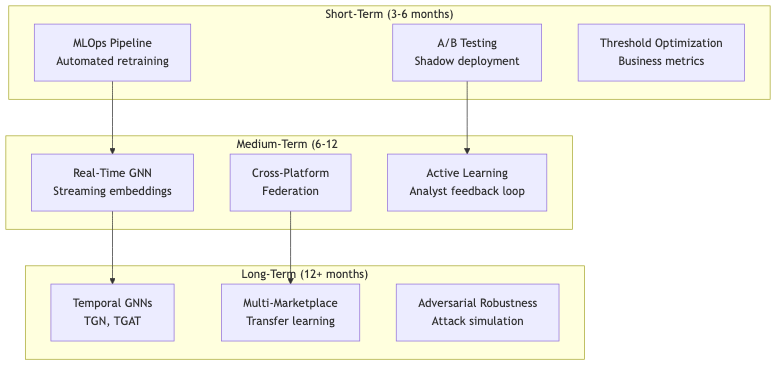
\includegraphics[width=0.8\textwidth]{figures/fig_6_1.png}
    \caption{Future Research Directions}
    \label{fig:6_1}
\end{figure}

\textbf{Short-Term Extensions:}
\begin{itemize}
    \item MLOps pipeline with automated monthly retraining and DDM/ADWIN-triggered updates
    \item Shadow deployment comparing our model against SEON in production
    \item Threshold optimization based on business metrics (investigation capacity, fraud loss)
\end{itemize}

\textbf{Medium-Term Research:}
\begin{itemize}
    \item Real-time GNN inference with incremental graph updates for streaming predictions
    \item Cross-platform federation sharing fraud signals between Homegate and ImmoScout24
    \item Active learning incorporating fraud analyst feedback to improve labels
\end{itemize}

\textbf{Long-Term Directions:}
\begin{itemize}
    \item Temporal GNNs (TGN, TGAT) capturing time-evolving fraud patterns
    \item Transfer learning across European marketplace platforms
    \item Adversarial robustness testing against adaptive fraudsters
\end{itemize}

\section{Closing Remarks}
\label{sec:6_5}

This research demonstrates that graph-based pattern discovery provides actionable fraud intelligence beyond traditional tabular approaches. The +5.3\% AUC-PR improvement validates relational patterns as complementary signals, while SHAP-based explanations bridge the gap between model predictions and analyst investigations. As fraud tactics evolve, the combination of graph mining, temporal validation, and interpretable models offers a foundation for adaptive, trustworthy fraud detection systems.



\printbibliography[title={References}]

% Appendices
\appendix
\chapter{Configuration Files}
\label{appendix:configurations}

This appendix provides complete Hydra configuration files used throughout the implementation.

\section{Training Configuration}
\label{appendix:train_config}

Complete training configuration file (\texttt{configs/experiment.yaml}):

\begin{lstlisting}[language=yaml, basicstyle=\ttfamily\fontsize{9}{11}\selectfont]
experiment:
  name: "fraud_detection"
  tracking_uri: "sqlite:///mlflow.db"

data:
  path: "artifacts/merged_events.parquet"
  train_start_date: "2024-12-01"
  train_end_date: "2025-06-01"
  test_end_date: "2025-07-01"

training:
  mode: "single"  # or "expanding"
  gap_days: 7
  run_shap: false

model:
  variant: "gnn_xgboost"  # vanilla_xgboost, gnn_xgboost
  xgboost:
    n_estimators: 100
    max_depth: 3
    learning_rate: 0.1
    min_child_weight: 1
    subsample: 1.0
    colsample_bytree: 1.0
    scale_pos_weight: 11.0
    eval_metric: "aucpr"
  gnn:
    hidden_dim: 32
    output_dim: 16
    num_layers: 2
    epochs: 5
    learning_rate: 0.01
    dropout: 0.3
\end{lstlisting}

\section{Hyperparameter Optimization Configuration}
\label{appendix:hpo_config}

XGBoost HPO configuration (\texttt{configs/hpo\_xgboost.yaml}):

\begin{lstlisting}[language=yaml, basicstyle=\ttfamily\fontsize{9}{11}\selectfont]
# configs/hpo_xgboost.yaml
defaults:
  - experiment

hydra:
  sweeper:
    _target_: hydra_plugins.hydra_optuna_sweeper.optuna_sweeper.OptunaSweeper
    n_trials: 50
    direction: maximize
    sampler:
      _target_: optuna.samplers.TPESampler
      seed: 42
    params:
      model.xgboost.n_estimators: range(50, 500, step=50)
      model.xgboost.max_depth: range(3, 12)
      model.xgboost.learning_rate: interval(0.01, 0.3)
      model.xgboost.min_child_weight: range(1, 10)
      model.xgboost.subsample: interval(0.6, 1.0)
      model.xgboost.colsample_bytree: interval(0.6, 1.0)
      model.xgboost.scale_pos_weight: interval(1.0, 20.0)
\end{lstlisting}

Joint GNN+XGBoost HPO configuration (\texttt{configs/hpo\_gnn\_xgboost.yaml}):

\begin{lstlisting}[language=yaml, basicstyle=\ttfamily\fontsize{9}{11}\selectfont]
# configs/hpo_gnn_xgboost.yaml
defaults:
  - experiment

model:
  variant: "gnn_xgboost"
  # Fix XGBoost params from Stage 1 optimization
  xgboost:
    max_depth: 5
    learning_rate: 0.085
    n_estimators: 200

hydra:
  sweeper:
    _target_: hydra_plugins.hydra_optuna_sweeper.optuna_sweeper.OptunaSweeper
    n_trials: 30
    direction: maximize
    sampler:
      _target_: optuna.samplers.TPESampler
      seed: 42
    params:
      model.gnn.hidden_dim: choice(16, 32, 64)
      model.gnn.output_dim: choice(8, 16, 32)
      model.gnn.num_layers: choice(2, 3)
      model.gnn.learning_rate: interval(0.001, 0.01)
      model.gnn.dropout: interval(0.1, 0.5)
\end{lstlisting}

\section{ETL Pipeline Configuration}
\label{appendix:etl_config}

Data pipeline configuration (\texttt{conf/config.yaml}):

\begin{lstlisting}[language=yaml, basicstyle=\ttfamily\fontsize{9}{11}\selectfont]
# conf/config.yaml
defaults:
  - data: default

output:
  dir: "artifacts"
  merged_file: "merged_events.parquet"

processing:
  chunk_size: 10000
  anonymize_pii: true
  compression: "snappy"
\end{lstlisting}

Data source configuration (\texttt{conf/data/default.yaml}):

\begin{lstlisting}[language=yaml, basicstyle=\ttfamily\fontsize{9}{11}\selectfont]
# conf/data/default.yaml
events:
  path: "data/raw/listing_events.parquet"
  datetime_format: "%Y-%m-%d %H:%M:%S.%f %z"

seon:
  path: "data/raw/seon_transactions.parquet"
  datetime_format: "%Y-%m-%dT%H:%M:%S.%f%z"

labels:
  path: "data/raw/fraud_labels.parquet"
  positive_class: "FRAUD"

column_mappings:
  event_id: "INSERTION_ID"
  timestamp: "event_dt"
  user_id: "USER_ID"
  device_hash: "device_fingerprint_hash"
  ip_hash: "ip_address_hash"
\end{lstlisting}

\chapter{Implementation Code}
\label{appendix:implementations}

This appendix provides complete Python implementations referenced in Chapter~4.

\section{Graph Construction}
\label{appendix:graph_construction}

Heterogeneous graph builder (\texttt{src/features/graph\_builder.py}):

\begin{lstlisting}[language=Python, basicstyle=\ttfamily\fontsize{8}{10}\selectfont]
import polars as pl
import torch
from torch_geometric.data import HeteroData

class HeterogeneousGraphBuilder:
    def __init__(self, entity_types=["device", "ip", "email", "phone", "user"]):
        self.entity_types = entity_types

    def build_graph(self, events_df: pl.DataFrame, cutoff_date: str) -> HeteroData:
        """Build heterogeneous graph with listing nodes and entity-sharing edges."""
        # Filter events before cutoff
        filtered = events_df.filter(pl.col("event_dt") <= cutoff_date)

        # Initialize graph
        graph = HeteroData()

        # Extract node features (44 dims: 36 base + 8 temporal)
        features = self._extract_node_features(filtered)
        graph["listing"].x = torch.tensor(features.to_numpy(), dtype=torch.float)

        # Build edges for each entity type
        for entity_type in self.entity_types:
            edge_index = self._build_sharing_edges(filtered, entity_type)
            graph["listing", f"shares_{entity_type}", "listing"].edge_index = edge_index

        return graph

    def _build_sharing_edges(self, df: pl.DataFrame, entity_type: str) -> torch.Tensor:
        """Create edges between listings sharing the same entity."""
        col_name = f"{entity_type}_hash"

        # Group by entity, get listing IDs
        entity_groups = (
            df.groupby(col_name)
            .agg(pl.col("listing_id").unique())
            .filter(pl.col("listing_id").list.len() > 1)  # Only shared entities
        )

        # Create edges (all pairs within each group)
        edge_list = []
        for group in entity_groups.iter_rows():
            listings = group[1]
            for i, src in enumerate(listings):
                for dst in listings[i+1:]:
                    edge_list.append([src, dst])
                    edge_list.append([dst, src])  # Undirected

        return torch.tensor(edge_list, dtype=torch.long).t()
\end{lstlisting}

Neighbor sampling configuration:

\begin{lstlisting}[language=Python, basicstyle=\ttfamily\fontsize{8}{10}\selectfont]
from torch_geometric.loader import NeighborLoader

# 2-hop neighborhood sampling for training
loader = NeighborLoader(
    graph,
    num_neighbors=[15, 10],  # 15 neighbors at layer 1, 10 at layer 2
    batch_size=512,
    input_nodes=("listing", train_mask),
    shuffle=True,
)
\end{lstlisting}

\section{Hybrid Training Pipeline}
\label{appendix:hybrid_training}

Complete hybrid pipeline (\texttt{src/training/hybrid.py}):

\begin{lstlisting}[language=Python, basicstyle=\ttfamily\fontsize{8}{10}\selectfont]
import numpy as np
import torch
import xgboost as xgb

def train_hybrid_pipeline(train_df, graph, gnn_model, best_params):
    """Train hybrid GNN+XGBoost pipeline."""
    # Stage 1: Generate GNN embeddings
    gnn_model.eval()
    with torch.no_grad():
        embeddings = gnn_model(graph.x_dict, graph.edge_index_dict)
        listing_emb = embeddings["listing"].cpu().numpy()  # [N, 16]

    # Stage 2: Concatenate with tabular features
    tabular_features = train_df[FEATURE_COLUMNS].to_numpy()  # [N, 65]
    combined_features = np.hstack([tabular_features, listing_emb])  # [N, 81]

    # Stage 3: Train XGBoost
    model = xgb.XGBClassifier(**best_params)
    model.fit(
        combined_features,
        train_df["is_fraud"].to_numpy(),
        eval_set=[(X_val, y_val)],
        early_stopping_rounds=10,
        verbose=False
    )

    return model
\end{lstlisting}

\section{Hyperparameter Optimization}
\label{appendix:hpo}

Optuna objective function (\texttt{src/training/hpo.py}):

\begin{lstlisting}[language=Python, basicstyle=\ttfamily\fontsize{8}{10}\selectfont]
import optuna
from optuna.samplers import TPESampler
from sklearn.metrics import average_precision_score

def objective(trial, X_train, y_train, X_val, y_val):
    """Optuna objective for XGBoost hyperparameter optimization."""
    params = {
        "n_estimators": trial.suggest_int("n_estimators", 50, 500, step=50),
        "max_depth": trial.suggest_int("max_depth", 3, 12),
        "learning_rate": trial.suggest_float("learning_rate", 0.01, 0.3, log=True),
        "min_child_weight": trial.suggest_int("min_child_weight", 1, 10),
        "subsample": trial.suggest_float("subsample", 0.6, 1.0),
        "colsample_bytree": trial.suggest_float("colsample_bytree", 0.6, 1.0),
        "scale_pos_weight": trial.suggest_float("scale_pos_weight", 1.0, 20.0),
        "eval_metric": "aucpr",
    }

    model = xgb.XGBClassifier(**params, random_state=42)
    model.fit(
        X_train, y_train,
        eval_set=[(X_val, y_val)],
        early_stopping_rounds=10,
        verbose=False
    )

    y_pred_proba = model.predict_proba(X_val)[:, 1]
    return average_precision_score(y_val, y_pred_proba)

# Run optimization
study = optuna.create_study(direction="maximize", sampler=TPESampler(seed=42))
study.optimize(lambda trial: objective(trial, X_train, y_train, X_val, y_val), n_trials=50)
best_params = study.best_params
\end{lstlisting}

\section{Drift Detection}
\label{appendix:drift_detection}

DDM implementation (\texttt{src/evaluation/drift.py}):

\begin{lstlisting}[language=Python, basicstyle=\ttfamily\fontsize{8}{10}\selectfont]
import numpy as np

class DDM:
    """Drift Detection Method."""
    def __init__(self, warning_threshold=2.0, drift_threshold=3.0):
        self.warning_threshold = warning_threshold
        self.drift_threshold = drift_threshold
        self.errors = []

    def update(self, prediction, true_label):
        """Update with new prediction and return drift status."""
        error = int(prediction != true_label)
        self.errors.append(error)

        # Compute error rate statistics
        p = np.mean(self.errors)
        s = np.sqrt(p * (1 - p) / len(self.errors))

        # Check for drift
        if p + s >= self.drift_threshold:
            self.errors = []  # Reset on drift
            return "DRIFT"
        elif p + s >= self.warning_threshold:
            return "WARNING"
        return "STABLE"
\end{lstlisting}

ADWIN implementation:

\begin{lstlisting}[language=Python, basicstyle=\ttfamily\fontsize{8}{10}\selectfont]
import numpy as np

class ADWIN:
    """Adaptive Windowing drift detector."""
    def __init__(self, delta=0.002):
        self.delta = delta
        self.window = []

    def update(self, prediction, true_label):
        """Update with new prediction and return drift status."""
        error = int(prediction != true_label)
        self.window.append(error)

        # Check all possible splits
        for i in range(1, len(self.window)):
            left = self.window[:i]
            right = self.window[i:]

            if self._detect_change(left, right):
                self.window = self.window[i:]  # Drop old data
                return "DRIFT"

        return "STABLE"

    def _detect_change(self, left, right):
        """Statistical test for distribution change."""
        mu_left = np.mean(left)
        mu_right = np.mean(right)

        n_left = len(left)
        n_right = len(right)
        m = 1 / (1/n_left + 1/n_right)

        var = mu_left * (1 - mu_left) / n_left + mu_right * (1 - mu_right) / n_right
        epsilon_cut = np.sqrt(2 * var * np.log(2 / self.delta) / m)

        return abs(mu_left - mu_right) > epsilon_cut
\end{lstlisting}

\section{Evaluation Metrics}
\label{appendix:metrics}

Metric computation (\texttt{src/utils/metrics.py}):

\begin{lstlisting}[language=Python, basicstyle=\ttfamily\fontsize{8}{10}\selectfont]
from sklearn.metrics import (
    average_precision_score,
    roc_auc_score,
    precision_recall_curve,
    precision_score,
    recall_score,
    f1_score,
)
import numpy as np

def compute_metrics(y_true, y_pred_proba, threshold=0.5):
    """Compute comprehensive evaluation metrics."""
    y_pred = (y_pred_proba >= threshold).astype(int)

    metrics = {
        "auc_pr": average_precision_score(y_true, y_pred_proba),
        "auc_roc": roc_auc_score(y_true, y_pred_proba),
        "precision": precision_score(y_true, y_pred),
        "recall": recall_score(y_true, y_pred),
        "f1": f1_score(y_true, y_pred),
        "precision@50": precision_at_k(y_true, y_pred_proba, k=50),
        "precision@100": precision_at_k(y_true, y_pred_proba, k=100),
        "precision@200": precision_at_k(y_true, y_pred_proba, k=200),
    }

    return metrics

def precision_at_k(y_true, y_scores, k):
    """Compute precision at top-K predictions."""
    sorted_indices = np.argsort(-y_scores)[:k]
    top_k_labels = y_true[sorted_indices]
    return np.sum(top_k_labels) / k
\end{lstlisting}

\section{Feature Engineering}
\label{appendix:feature_engineering}

Cyclical encoding (\texttt{src/features/temporal.py}):

\begin{lstlisting}[language=Python, basicstyle=\ttfamily\fontsize{8}{10}\selectfont]
import numpy as np
import polars as pl

def apply_cyclical_encoding(df: pl.DataFrame) -> pl.DataFrame:
    """Apply cyclical encoding to temporal features."""
    return df.with_columns([
        # Hour encoding (0-23)
        (2 * np.pi * pl.col("event_hour") / 24).sin().alias("hour_sin"),
        (2 * np.pi * pl.col("event_hour") / 24).cos().alias("hour_cos"),
        # Weekday encoding (0-6)
        (2 * np.pi * pl.col("event_day_of_week") / 7).sin().alias("weekday_sin"),
        (2 * np.pi * pl.col("event_day_of_week") / 7).cos().alias("weekday_cos"),
    ])
\end{lstlisting}

Feature schema (\texttt{src/features/schema.py}):

\begin{lstlisting}[language=Python, basicstyle=\ttfamily\fontsize{8}{10}\selectfont]
from dataclasses import dataclass
from typing import List

@dataclass
class FeatureSchema:
    """Feature schema for fraud detection models."""
    seon_boolean: List[str]
    seon_categorical: List[str]
    listing_numeric: List[str]
    listing_categorical: List[str]
    temporal: List[str]

    @property
    def all_features(self) -> List[str]:
        """Return all feature names."""
        return (
            self.seon_boolean
            + self.seon_categorical
            + self.listing_numeric
            + self.listing_categorical
            + self.temporal
        )

    @property
    def categorical_features(self) -> List[str]:
        """Return categorical feature names."""
        return self.seon_categorical + self.listing_categorical

    @property
    def boolean_features(self) -> List[str]:
        """Return boolean feature names."""
        return self.seon_boolean
\end{lstlisting}

\section{ETL Pipeline}
\label{appendix:etl}

As-of join implementation (\texttt{src/data/transform.py}):

\begin{lstlisting}[language=Python, basicstyle=\ttfamily\fontsize{8}{10}\selectfont]
import polars as pl
from typing import Tuple, Dict

def correlate_events_to_seon(
    events_df: pl.DataFrame,
    seon_df: pl.DataFrame,
    seon_unique_col: str = "id",
) -> Tuple[pl.DataFrame, Dict[str, int]]:
    """Correlate each event to closest SEON transaction by timestamp."""

    # Sort both dataframes
    events_sorted = events_df.sort(["INSERTION_ID", "event_dt"])
    seon_sorted = seon_df.sort(["INSERTION_ID", "seon_dt"])

    # Prepare SEON dataframe for join
    seon_for_join = seon_sorted.select([
        "INSERTION_ID", "seon_dt",
        pl.col(seon_unique_col).alias("seon_id"),
        *[col for col in seon_df.columns if col not in ["INSERTION_ID", "seon_dt", seon_unique_col]]
    ])

    # Forward join: closest SEON after the event
    fwd_cols = (
        events_sorted
        .join_asof(
            seon_for_join,
            left_on="event_dt",
            right_on="seon_dt",
            by="INSERTION_ID",
            strategy="forward",
            suffix="_fwd"
        )
    )

    # Backward join: closest SEON before the event
    bwd_cols = (
        events_sorted
        .join_asof(
            seon_for_join,
            left_on="event_dt",
            right_on="seon_dt",
            by="INSERTION_ID",
            strategy="backward",
            suffix="_bwd"
        )
    )

    # Merge and prefer forward match
    merged = fwd_cols.join(
        bwd_cols.select(["INSERTION_ID", "event_dt"] +
                       [col for col in bwd_cols.columns if col.endswith("_bwd")]),
        on=["INSERTION_ID", "event_dt"],
        how="left"
    )

    # Coalesce: prefer forward, fallback to backward
    final_cols = []
    for col in seon_for_join.columns:
        if col not in ["INSERTION_ID", "seon_dt"]:
            final_cols.append(
                pl.coalesce([pl.col(f"{col}_fwd"), pl.col(f"{col}_bwd")]).alias(col)
            )

    result = merged.with_columns(final_cols)

    return result
\end{lstlisting}

\section{MLflow Integration}
\label{appendix:mlflow}

Training with MLflow logging (\texttt{src/training/trainer.py}):

\begin{lstlisting}[language=Python, basicstyle=\ttfamily\fontsize{8}{10}\selectfont]
import mlflow
from omegaconf import OmegaConf

def train_with_mlflow(cfg, pipeline):
    """Train model with MLflow experiment tracking."""

    # Configure MLflow
    mlflow.set_tracking_uri(cfg.experiment.tracking_uri)
    mlflow.set_experiment(cfg.experiment.name)

    # Start run
    run_name = f"{cfg.model.variant}_{cfg.data.train_start_date}"
    with mlflow.start_run(run_name=run_name):

        # Log hyperparameters
        params_dict = OmegaConf.to_container(cfg, resolve=True)
        mlflow.log_params(flatten_dict(params_dict))

        # Train model
        result = pipeline.run()

        # Log metrics
        mlflow.log_metrics({
            "train_auc_pr": result.train_metrics.auc_pr,
            "train_auc_roc": result.train_metrics.auc_roc,
            "val_auc_pr": result.val_metrics.auc_pr,
            "test_auc_pr": result.test_metrics.auc_pr,
            "test_precision@50": result.test_metrics.precision_at_50,
            "test_precision@100": result.test_metrics.precision_at_100,
            "training_time_seconds": result.training_time,
        })

        # Log model artifact
        mlflow.xgboost.log_model(result.model, "model")

        # Log SHAP plots if enabled
        if cfg.training.run_shap:
            mlflow.log_artifact(result.shap_summary_plot, "shap_summary.png")

        return result

def flatten_dict(d, parent_key='', sep='_'):
    """Flatten nested dictionary for MLflow logging."""
    items = []
    for k, v in d.items():
        new_key = f"{parent_key}{sep}{k}" if parent_key else k
        if isinstance(v, dict):
            items.extend(flatten_dict(v, new_key, sep=sep).items())
        else:
            items.append((new_key, v))
    return dict(items)
\end{lstlisting}

\section{API Service}
\label{appendix:api}

FastAPI endpoint (\texttt{src/api/main.py}):

\begin{lstlisting}[language=Python, basicstyle=\ttfamily\fontsize{8}{10}\selectfont]
from fastapi import FastAPI, HTTPException
from pydantic import BaseModel
import xgboost as xgb
import shap

app = FastAPI(title="Fraud Detection API")

# Load model at startup
model = xgb.Booster()
model.load_model("models/production_model.json")
explainer = shap.TreeExplainer(model)

class EventPayload(BaseModel):
    insertion_id: str
    device_hash: str
    ip_hash: str
    email_hash: str
    # ... other features

class PredictResponse(BaseModel):
    probability: float
    risk_level: str
    top_factors: list

@app.post("/predict")
async def predict(event: EventPayload) -> PredictResponse:
    """Generate fraud prediction with explanation."""
    try:
        # Extract features
        features = feature_engineer.extract(event, event_store)

        # Enrich with graph-like counts
        features["device_link_count"] = event_store.count_related("device", event.device_hash)
        features["ip_link_count"] = event_store.count_related("ip", event.ip_hash)
        features["email_link_count"] = event_store.count_related("email", event.email_hash)

        # Generate prediction
        dmatrix = xgb.DMatrix([features])
        prob = model.predict(dmatrix)[0]

        # Compute SHAP values
        shap_values = explainer.shap_values(dmatrix)
        top_factors = get_top_factors(shap_values[0], feature_names, k=5)

        # Determine risk level
        if prob > 0.7:
            risk_level = "HIGH"
        elif prob > 0.3:
            risk_level = "MEDIUM"
        else:
            risk_level = "LOW"

        return PredictResponse(
            probability=float(prob),
            risk_level=risk_level,
            top_factors=top_factors
        )

    except Exception as e:
        raise HTTPException(status_code=500, detail=str(e))

def get_top_factors(shap_values, feature_names, k=5):
    """Get top-K contributing factors."""
    importance = [(name, abs(val)) for name, val in zip(feature_names, shap_values)]
    importance.sort(key=lambda x: x[1], reverse=True)
    return [{"feature": name, "importance": float(val)} for name, val in importance[:k]]
\end{lstlisting}

\section{GNN Implementation}
\label{appendix:gnn}

GraphSAGE encoder (\texttt{src/models/graphsage.py}):

\begin{lstlisting}[language=Python, basicstyle=\ttfamily\fontsize{8}{10}\selectfont]
import torch
import torch.nn as nn
import torch.nn.functional as F
from torch_geometric.nn import SAGEConv, HeteroConv

class GraphSAGEEncoder(torch.nn.Module):
    """GraphSAGE encoder for heterogeneous graphs."""

    def __init__(self, in_channels, hidden_channels, out_channels,
                 num_layers, dropout, edge_types):
        super().__init__()
        self.convs = nn.ModuleList()

        for i in range(num_layers):
            in_ch = in_channels if i == 0 else hidden_channels
            out_ch = out_channels if i == num_layers - 1 else hidden_channels

            # Create SAGEConv for each edge type
            conv_dict = {
                ("listing", edge_type, "listing"): SAGEConv(in_ch, out_ch, aggr="mean")
                for edge_type in edge_types
            }
            self.convs.append(HeteroConv(conv_dict, aggr="sum"))

        self.dropout = dropout

    def forward(self, x_dict, edge_index_dict):
        """Forward pass through GNN layers."""
        x = x_dict
        for i, conv in enumerate(self.convs):
            x = conv(x, edge_index_dict)
            if i < len(self.convs) - 1:  # No activation/dropout on last layer
                x = {k: F.relu(v) for k, v in x.items()}
                x = {k: F.dropout(v, p=self.dropout, training=self.training)
                     for k, v in x.items()}

        return x["listing"]

def train_supervised(model, loader, optimizer, device, epochs=30):
    """Supervised GNN training loop."""
    model.train()
    for epoch in range(epochs):
        total_loss = 0
        for batch in loader:
            batch = batch.to(device)
            optimizer.zero_grad()

            # Forward pass
            out = model(batch.x_dict, batch.edge_index_dict)

            # Compute loss on training nodes
            loss = F.binary_cross_entropy_with_logits(
                out[batch["listing"].train_mask],
                batch["listing"].y[batch["listing"].train_mask],
                pos_weight=torch.tensor([11.0], device=device)  # Class imbalance
            )

            # Backward pass
            loss.backward()
            optimizer.step()

            total_loss += loss.item()

        avg_loss = total_loss / len(loader)
        print(f"Epoch {epoch+1}/{epochs}, Loss: {avg_loss:.4f}")
\end{lstlisting}


\end{document}
